\documentclass[12pt,a4paper]{article}
\usepackage[utf8]{inputenc}
\usepackage[vietnamese]{babel}
\usepackage{amsmath,amssymb,amsfonts}
\usepackage{graphicx}
\usepackage{float}
\usepackage{booktabs}
\usepackage{hyperref}
\usepackage{tcolorbox}
\usepackage{geometry}
\usepackage{listings}
\usepackage{enumitem}

\geometry{margin=1in}

\hypersetup{
    colorlinks=true,
    linkcolor=blue,
    filecolor=magenta,      
    urlcolor=cyan,
    pdftitle={Phản biện thiết kế hệ thống --- Distributed Watermark Tracker},
    pdfpagemode=FullScreen,
}

\tcbuselibrary{theorems}
\tcbset{highlight math style={colback=yellow!5!white,colframe=orange!75!black,arc=1mm,boxrule=0.5pt,left=2pt,right=2pt,top=2pt,bottom=2pt}}

% Cấu hình đóng khung công thức toán độc lập
\newtcolorbox{mathframe}{
  colback=yellow!5!white,
  colframe=orange!75!black,
  arc=2mm,
  boxrule=1pt,
  left=5pt,
  right=5pt,
  top=5pt,
  bottom=5pt
}

\title{Phản biện thiết kế hệ thống --- Distributed Watermark Tracker}
\author{Distributed Watermark Tracker Team}
\date{\today}

\begin{document}

\maketitle
\tableofcontents
\newpage
Mỗi mục thiết kế được sắp xếp để đọc lần đầu vẫn nắm được ngay: \textbf{ý chính của thiết kế} $\rightarrow$ \textbf{bản đồ thiết kế} $\rightarrow$ \textbf{cách chạy từng bước} $\rightarrow$ \textbf{ví dụ vận hành} $\rightarrow$ \textbf{phản biện vì sao chọn như vậy}. Phần bản đồ luôn đi theo cùng thứ tự: thành phần, dữ liệu vào/ra, luồng xử lý, trạng thái cần giữ, giao tiếp và đầu ra. Mã sơ đồ tách riêng trong thư mục \href{mermaid/}{\texttt{mermaid/}}; tài liệu này chỉ trích dẫn.
> Render sơ đồ: \texttt{mmdc -i mermaid/<tên\_file>.mmd -o <tên\_file>.svg}, hoặc dán nội dung \texttt{.mmd} vào https://mermaid.live.
\textbf{Bài toán.} Gom luồng log đến bất tuần tự thành cửa sổ 5 giây trên event-time. Quyết định cốt lõi là \textit{chốt cửa sổ khi nào} — một đánh đổi giữa độ đầy đủ dữ liệu và độ trễ. Hai thiết kế watermark là hai lời giải ở hai đầu của đánh đổi này.

\section{Bảng ký hiệu và định nghĩa (Glossary)}
\label{sec:notations}
Dưới đây là bảng giải nghĩa các ký hiệu toán học, các biến trạng thái và thuật ngữ được sử dụng xuyên suốt tài liệu phản biện:

\begin{table}[H]
\centering
\begin{tabular}{p{4.5cm}p{10.5cm}}
\toprule
\textbf{Ký hiệu / Thuật ngữ} & \textbf{Ý nghĩa và định nghĩa trong thiết kế} \\
\midrule
\tcbhighmath{W_{global}} & Watermark toàn cục trong chế độ Strict, dùng để chốt cửa sổ trên toàn bộ Worker. \\
\tcbhighmath{W_{global\_h}} & Watermark toàn cục trong chế độ Heuristic, dùng để chốt cửa sổ tạm tính (speculative). \\
\tcbhighmath{W_{global\_h\_prev}} & Heuristic Watermark toàn cục ở chu kỳ trước đó. \\
\tcbhighmath{LW_i} & Local Watermark (watermark cục bộ) của partition \texttt{i}, tiến theo mốc punctuation nhận từ nguồn. \\
\tcbhighmath{W_h} & Heuristic Watermark (watermark dự đoán) cục bộ của partition, tính bằng cách lấy max event-time trừ đi độ trễ hiệu dụng. \\
\tcbhighmath{L_{eff}} & Effective Lateness (độ trễ hiệu dụng), ước lượng bằng phân vị \tcbhighmath{p} (ví dụ p99) của độ trễ thực tế thông qua DDSketch. \\
\tcbhighmath{T_{commit}} & Mốc thời gian cam kết được mang bởi Punctuation Token từ Ingestor, chứng minh không còn dữ liệu cũ hơn. \\
\tcbhighmath{T_{event}} & Thời điểm xảy ra sự kiện của bản ghi log (event-time). \\
\tcbhighmath{arrival\_time} & Thời điểm bản ghi được nhận vào hệ thống (thời gian thực tế của log). \\
\tcbhighmath{window\_end} & Thời điểm kết thúc cửa sổ thời gian (window-end). \\
\tcbhighmath{window\_start} & Thời điểm bắt đầu cửa sổ thời gian (window-start). \\
\tcbhighmath{max\_event\_time} & Thời điểm sự kiện lớn nhất đã quan sát được trong partition. \\
\tcbhighmath{W_{h\_prev}} & Heuristic Watermark cục bộ ở chu kỳ trước đó. \\
\tcbhighmath{W_{h\_raw}} & Heuristic Watermark cục bộ thô trước khi áp dụng rate limit hoặc hysteresis. \\
\tcbhighmath{W_{candidate}} & Watermark ứng viên đề xuất trước khi chốt đơn điệu. \\
\tcbhighmath{now} & Thời điểm xử lý sự kiện tại Worker Node (thời gian hệ thống). \\
\tcbhighmath{p} & Phân vị cấu hình để tính độ trễ hiệu dụng (ví dụ \tcbhighmath{p = 0.99} cho p99 \tcbhighmath{lateness}). \\
\tcbhighmath{e} & Event hiện tại hoặc bản ghi log đang được xử lý. \\
\tcbhighmath{offset} & Vị trí \tcbhighmath{offset} của bản ghi trong phân vùng Kafka. \\
\tcbhighmath{term} & Chỉ số epoch/fencing \tcbhighmath{term} hiện tại của Coordinator, dùng để chống các lệnh reassign trùng lặp hoặc cũ. \\
\tcbhighmath{delta} & Chênh lệch giá trị tích lũy do late event tạo ra trong correction. \\
\tcbhighmath{window\_id} & Định danh duy nhất của cửa sổ thời gian (thường ghép từ \tcbhighmath{partition\_id}, \tcbhighmath{window\_start}, \tcbhighmath{window\_end} và mode). \\
\tcbhighmath{partition\_id} & Định danh phân vùng dữ liệu Kafka. \\
\tcbhighmath{worker\_id} & Định danh tiến trình xử lý (Worker Node). \\
\tcbhighmath{emit\_id} & Khóa chống trùng (idempotency key) cho một lần phát kết quả cửa sổ. \\
\tcbhighmath{offset\_range} & Khoảng \tcbhighmath{offset} Kafka đã đóng góp dữ liệu vào một cửa sổ. \\
\tcbhighmath{watermark\_at\_close} & Giá trị watermark tại thời điểm đóng cửa sổ. \\
\tcbhighmath{original\_result\_version} & Phiên bản kết quả cửa sổ đã phát trước đó. \\
\tcbhighmath{correction\_id} & Khóa chống trùng cho một bản ghi hiệu chỉnh (correction). \\
\tcbhighmath{correction\_version} & Phiên bản của kết quả cửa sổ sau khi áp dụng hiệu chỉnh. \\
\tcbhighmath{lateness} & Độ trễ của sự kiện, tính bằng \tcbhighmath{now - event\_time}. \\
\tcbhighmath{max\_wait\_ms} & Thời gian chờ tối đa trong hàng đợi trước khi buộc phải xả (flush). \\
\tcbhighmath{sketch} & Cấu trúc dữ liệu DDSketch lưu trữ phân phối độ trễ. \\
\texttt{Worker} & Nút xử lý dữ liệu trong hệ thống phân tán, nhận dữ liệu từ Kafka, sắp xếp các bản ghi theo thời gian sự kiện, tính toán watermark cục bộ và lưu trữ trạng thái. \\
\texttt{Coordinator} & Thành phần điều khiển trong cấu hình Strict, tính toán watermark toàn cục dựa trên heartbeat từ các Worker và quản lý quyền sở hữu phân vùng (partition assignment). \\
\texttt{Aggregator} & Thành phần điều khiển trong cấu hình Heuristic, thu thập các watermark dự đoán (heuristic watermark) cục bộ và tổng hợp thành watermark toàn cục. \\
\texttt{Watermark} & Mốc thời gian logic biểu thị tiến độ thời gian sự kiện trong luồng dữ liệu. \\
\texttt{DDSketch} & Thuật toán phác thảo dữ liệu (data \tcbhighmath{sketch}) hiệu năng cao, ước lượng các phân vị (quantile) của độ trễ thực tế. \\
\texttt{DLQ (Dead Letter Queue)} & Hàng đợi chứa các sự kiện đến muộn sau khi cửa sổ thời gian tương ứng đã được chốt. \\
\texttt{Correction Message} & Thông điệp hiệu chỉnh được phát ra để cập nhật kết quả của một cửa sổ đã đóng. \\
\texttt{Punctuation Token} & Tín hiệu mốc thời gian sự kiện (\tcbhighmath{T_{commit}}) do Ingestor phát ra để khẳng định không còn sự kiện nào có mốc thời gian nhỏ hơn. \\
\texttt{Tiered Storage} & Cơ chế lưu trữ phân tầng chia làm 3 cấp: Tier-1 (RocksDB cục bộ), Tier-2 (Shared Volume để checkpoint), và Tier-3 (MinIO lưu trữ dài hạn). \\
\texttt{Failback} & Quy trình bàn giao an toàn các phân vùng xử lý từ Worker gánh hộ về lại Worker cũ sau khi Worker cũ đã phục hồi. \\
\bottomrule
\end{tabular}
\end{table}

\section{0. Khung phản biện trước khi vào thiết kế}
\label{sec:khung-phan-bien}
Trước khi trình bày từng thành phần, cần cố định bốn điểm để hội đồng hiểu đúng phạm vi thiết kế.
\textbf{Bài toán đầu vào.} Log không đến theo thứ tự event-time. Một bản ghi có \tcbhighmath{T_{event}} nhỏ vẫn có thể đến sau nhiều bản ghi mới hơn. Nếu chốt cửa sổ quá sớm thì mất dữ liệu; nếu chờ quá lâu thì latency tăng. Vì vậy hệ thống không chỉ là "đọc Kafka rồi group-by window", mà là bài toán quyết định thời điểm đóng cửa sổ dưới dữ liệu trễ.
\textbf{Ràng buộc thiết kế.}

\begin{table}[H]
\centering
\begin{tabular}{p{4.5cm}p{10.5cm}}
\toprule
\textbf{Ràng buộc} & \textbf{Ý nghĩa khi phản biện} \\
\midrule
Event-time window & Cửa sổ được tính theo thời điểm sự kiện, không theo thời điểm hệ thống nhận được log. \\
Out-of-order arrival & Cần watermark để biết khi nào đủ an toàn để chốt. \\
12 Kafka partition / 4 worker & Đơn vị đúng đắn nhỏ nhất là partition, không phải node. \\
Có crash/failover & State, \tcbhighmath{offset} và quyền sở hữu partition phải phục hồi được. \\
Hai mục tiêu khác nhau & Strict tối ưu correctness; Heuristic tối ưu latency và sửa sai bất đồng bộ. \\
\bottomrule
\end{tabular}
\end{table}
\textbf{Tiêu chí đánh giá.}

\begin{table}[H]
\centering
\begin{tabular}{p{3cm}p{6cm}p{6cm}}
\toprule
\textbf{Tiêu chí} & \textbf{Strict Watermark} & \textbf{Heuristic Watermark} \\
\midrule
Cam kết chính & Không mất dữ liệu trong đường xử lý chính & Latency thấp, chấp nhận late event tức thời \\
Cách chốt cửa sổ & Dựa trên Punctuation Token và \tcbhighmath{W_{global} = \min(LW_i)} & Dựa trên \tcbhighmath{L_{eff} = DDSketch.quantile(p)} và \tcbhighmath{W_h} \\
Dữ liệu đến muộn & Không được để xảy ra trong cửa sổ đã chốt nếu token đúng & Đưa vào DLQ và phát correction \\
Control plane & Coordinator HA/Raft vì có reassign/failback & Aggregator Active-Standby vì chỉ tổng hợp watermark \\
Khi nên dùng & Audit, billing, compliance, cần đúng ngay & Dashboard, phân tích gần real-time, cần latency thấp \\
\bottomrule
\end{tabular}
\end{table}
\textbf{Luận điểm xuyên suốt.} Mỗi phần "phức tạp" trong thiết kế phải trả lời được một câu hỏi rất cụ thể: nó bảo vệ cam kết nào? Nếu bỏ nó đi thì hỏng ở thuộc tính nào? Các mục dưới đây trình bày theo đúng hướng đó.
\textbf{Cách đọc từng mục thiết kế.}

\begin{table}[H]
\centering
\begin{tabular}{p{4.5cm}p{10.5cm}}
\toprule
\textbf{Phần trong mỗi mục} & \textbf{Người đọc cần nắm được} \\
\midrule
Ý chính & Mục này đang thiết kế thành phần nào và cam kết chính là gì. \\
Bản đồ thiết kế & Trình bày tách riêng từng thành phần, từng loại dữ liệu, từng state, từng kênh giao tiếp và từng output; không gộp nhiều ý vào một dòng. \\
Cách chạy từng bước & Event/control message đi qua hệ thống theo thứ tự nào, khi nào cập nhật state, khi nào emit kết quả. \\
Ví dụ vận hành & Một tình huống số cụ thể để kiểm tra người đọc đã hiểu đúng cơ chế. \\
Phản biện & Nêu rõ phản đề, vì sao phản đề nghe hợp lý, lý do bác bỏ, và kết luận thiết kế phải giữ thuộc tính nào. \\
\bottomrule
\end{tabular}
\end{table}
\textbf{Bức tranh tổng thể: 8 mục liên hệ với nhau thế nào.} Tám mục dưới đây không phải tám hệ thống rời rạc, mà là các chặng trên cùng một đường đi của một event:

\begin{enumerate}
\item Ingestor gắn event-time và (Strict) phát Punctuation, đẩy vào \textbf{Kafka} (\ref{sec:kafka-pq}).
\item Worker kéo event từ Kafka vào \textbf{Bounded PQ} để sắp theo event-time (\ref{sec:kafka-pq}), rồi đưa vào \textbf{engine của đúng partition} (\ref{sec:node-partition}).
\item Engine gom window và sinh \textbf{watermark cục bộ}: \tcbhighmath{LW_i} từ token (\ref{sec:strict-watermark}) hoặc \tcbhighmath{W_h} từ DDSketch (\ref{sec:heuristic-watermark}).
\item Watermark cục bộ đi qua \textbf{kênh control out-of-band} (\ref{sec:layer-communication}) lên \textbf{Coordinator} (Strict) hoặc \textbf{Aggregator} (Heuristic) (\ref{sec:coordinator-aggregator}) để hợp nhất thành watermark toàn cục.
\item Worker nhận watermark toàn cục, \textbf{đóng window} và phát kết quả; event đến muộn (Heuristic) đi vào DLQ (\ref{sec:strict-watermark}/\ref{sec:heuristic-watermark}).
\item Trạng thái được bền hóa qua \textbf{Tiered Storage} (\ref{sec:tiered-storage}); khi node chết, partition được bàn giao bằng \textbf{Failback} (\ref{sec:failback-5step}) dựa trên checkpoint Tier-2 và fencing token của Coordinator (\ref{sec:coordinator-aggregator}).
\end{enumerate}

\begin{figure}[H]
    \centering
    \makebox[\textwidth][c]{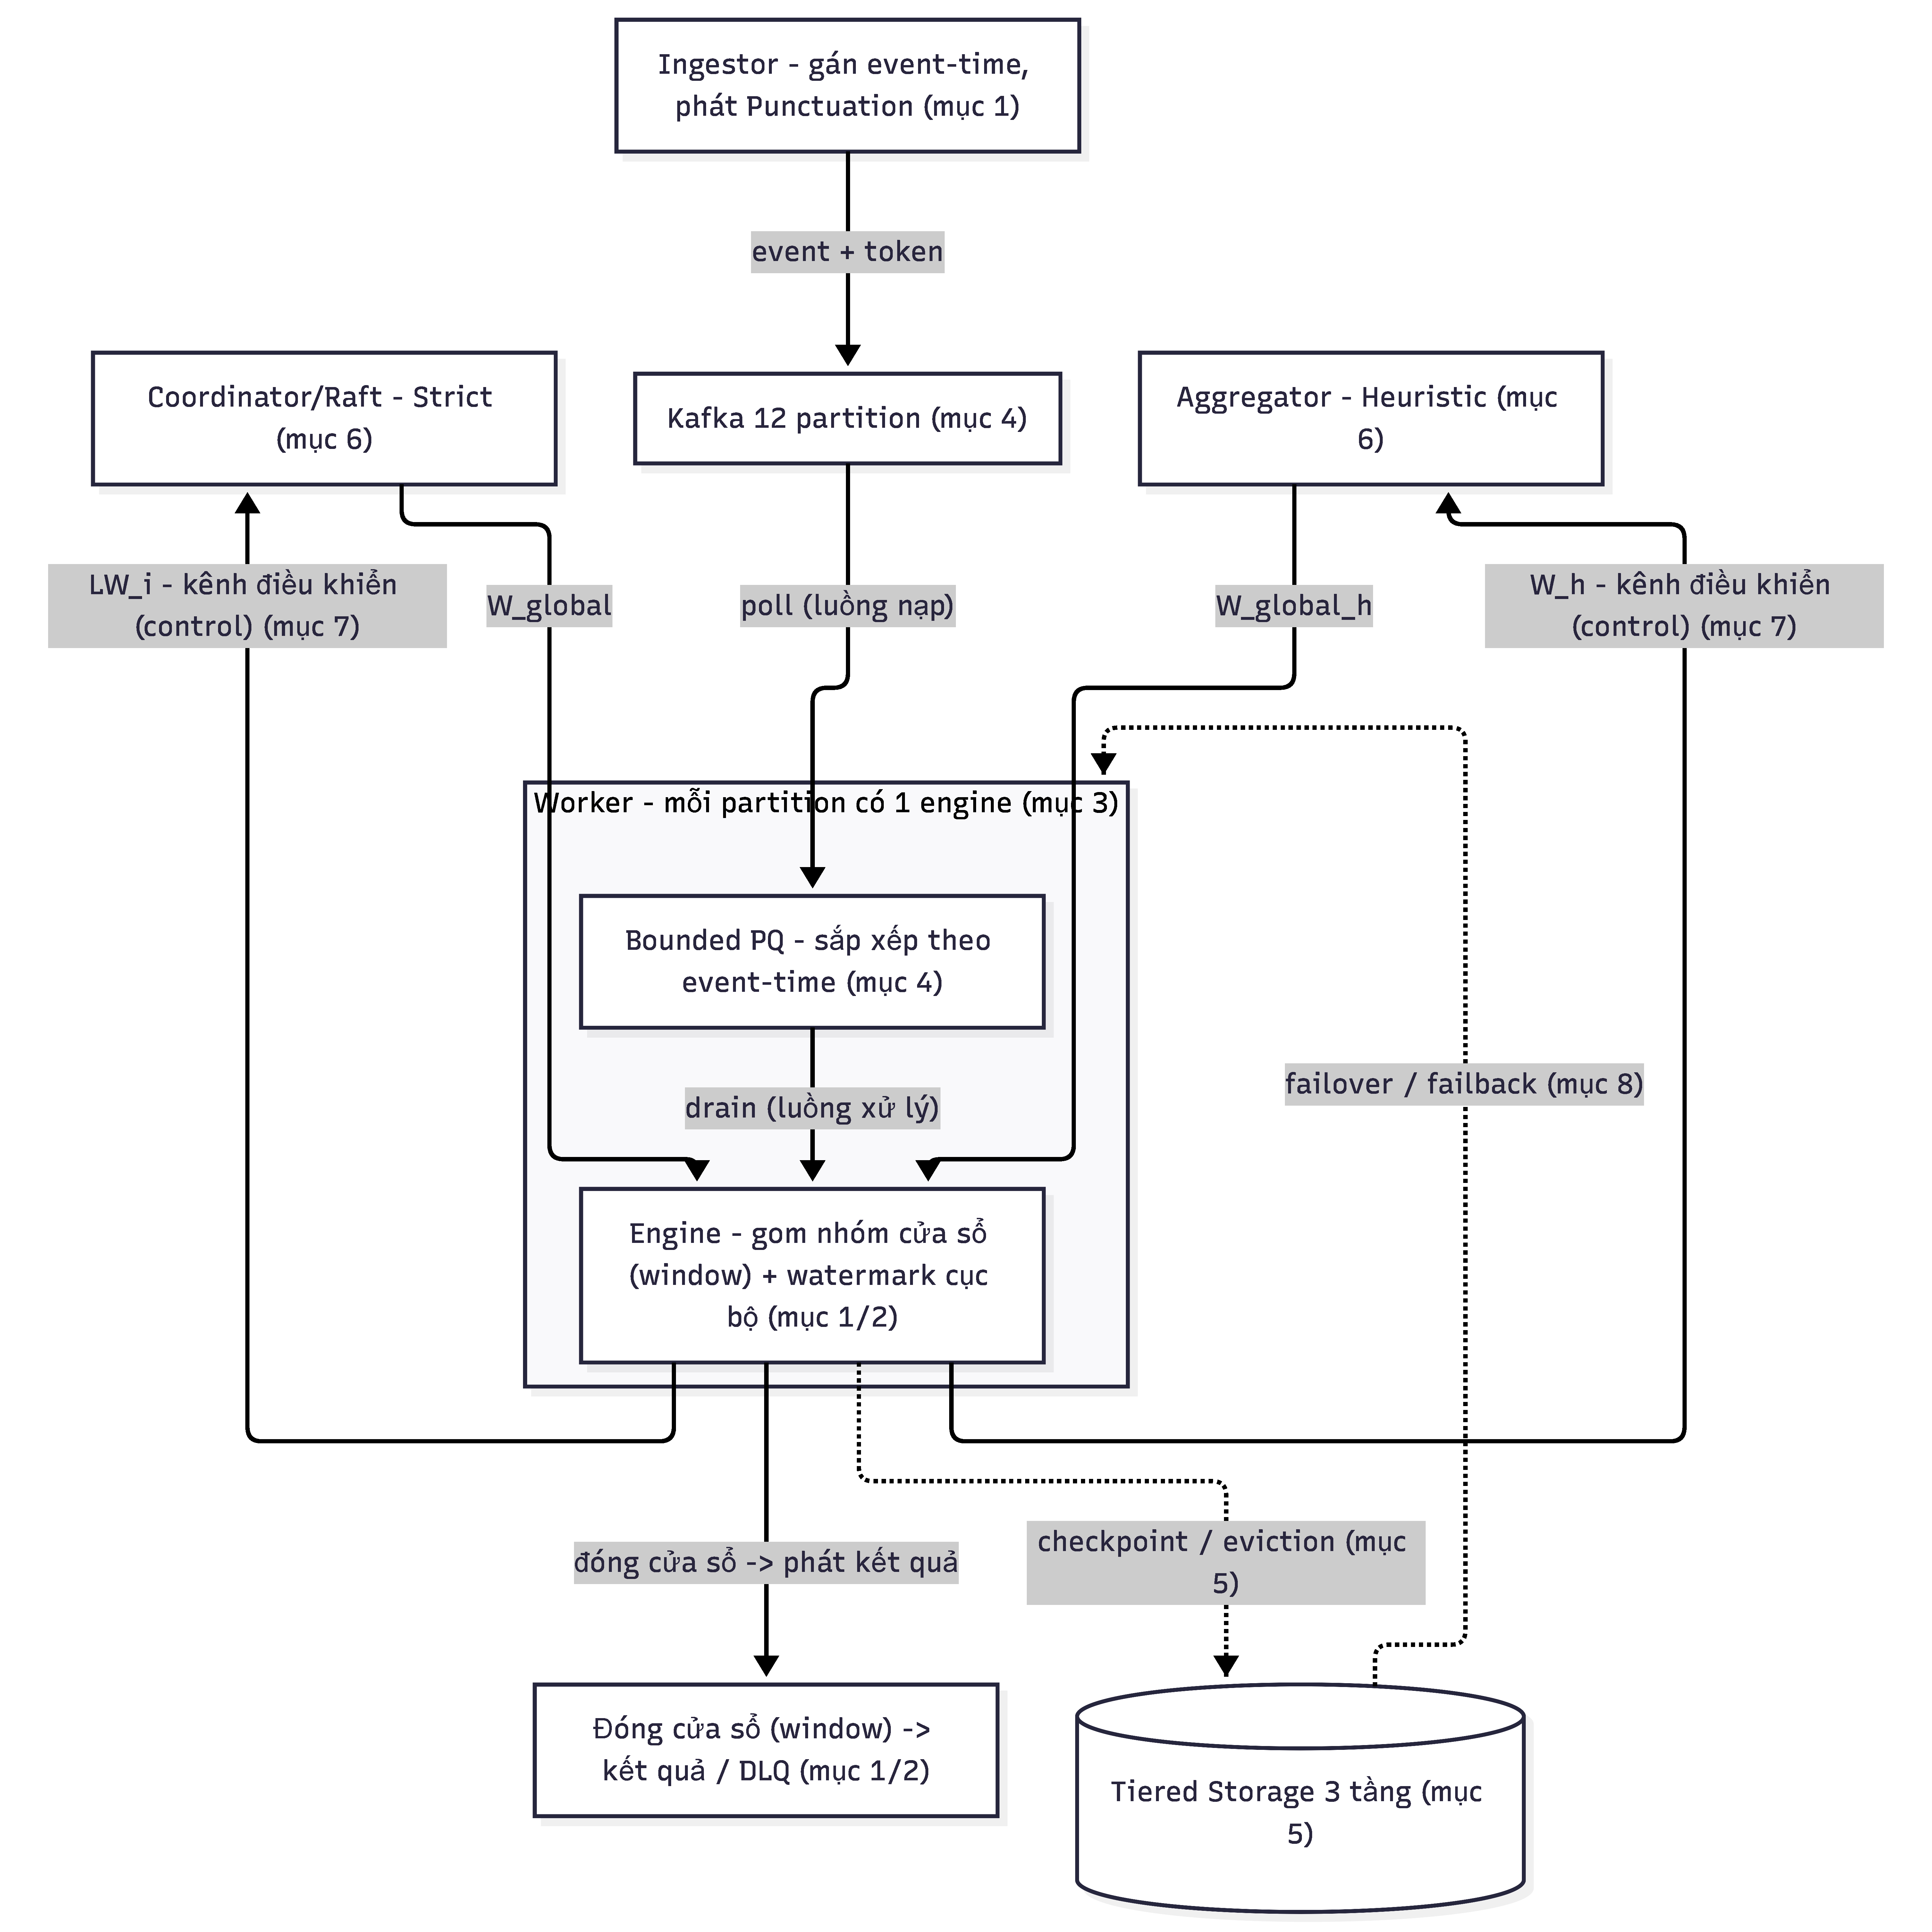
\includegraphics[width=1.15\textwidth]{end_to_end_pipeline.pdf}}
    \caption{Sơ đồ xâu chuỗi toàn hệ thống}
    \label{fig:end_to_end_pipeline}
\end{figure}
Cuối mỗi mục có dòng \textbf{Liên hệ} chỉ rõ mục đó nối với những mục nào, để khi đọc không tách rời khỏi tổng thể.

\section{1. Thiết kế Strict Watermark}
\label{sec:strict-watermark}

\subsection{1.1 Trình bày chi tiết thiết kế}
\textbf{Ý chính.} Strict Watermark là thiết kế ưu tiên tính đúng ngay tại thời điểm đóng cửa sổ. Watermark toàn cục chỉ được phép tiến khi \textit{mọi} partition đang hoạt động đã vượt qua cùng một mốc event-time. Nguồn tiến độ không phải là suy đoán từ Worker, mà là Punctuation Token do Ingestor phát ra. Coordinator hợp nhất local watermark theo công thức \tcbhighmath{W_{global} = \min(LW_i)}. Worker chỉ chốt cửa sổ khi \tcbhighmath{window\_end \le W_{global}}. Cam kết của mode này là không mất dữ liệu trong đường xử lý chính và bảo vệ exactly-once ở mức window output.
\textbf{Bản đồ thiết kế.}
\textbf{Thành phần và trách nhiệm.}

\begin{itemize}
\item \textbf{Ingestor:} đọc log đầu vào, gán log vào đúng Kafka partition, phát event và phát Punctuation Token cho từng partition.
\item \textbf{Kafka topic \texttt{events}:} giữ event và token theo thứ tự \tcbhighmath{offset} trong từng partition để Worker có thể replay.
\item \textbf{StrictWorker:} poll event/token theo partition, cfhuyển event vào engine đúng partition và gửi heartbeat lên Coordinator.
\item \textbf{StrictWatermarkEngine:} giữ open window, cập nhật aggregate, nhận token để tăng local watermark \tcbhighmath{LW_i}, đóng window khi đủ \tcbhighmath{W_{global}}.
\item \textbf{StrictCoordinator:} nhận heartbeat theo partition, tính \tcbhighmath{W_{global} = \min(LW_i)}, giữ watermark toàn cục đơn điệu.
\item \textbf{OutputManager:} phát \texttt{WindowResult} sang results/audit và chống phát trùng theo \tcbhighmath{window\_id}.
\end{itemize}
\textbf{Dữ liệu vào.}

\begin{itemize}
\item \textbf{Log/event:} bản ghi nghiệp vụ có \texttt{event\_time}, partition key và payload.
\item \textbf{Punctuation Token:} mốc \tcbhighmath{T_{commit}} chứng minh một partition đã phát hết event có \tcbhighmath{T_{event} \le T_{commit}}.
\item \textbf{Heartbeat từ Worker:} map \texttt{{\tcbhighmath{partition\_id} -> \tcbhighmath{LW_i}}} kèm trạng thái partition.
\end{itemize}
\textbf{Dữ liệu ra.}

\begin{itemize}
\item \textbf{Local watermark \tcbhighmath{LW_i}:} watermark cục bộ của từng partition.
\item \textbf{Global watermark \tcbhighmath{W_{global}}:} watermark toàn cục do Coordinator tính.
\item \textbf{\texttt{WindowResult}:} kết quả cửa sổ đã đóng, có \tcbhighmath{window\_id} để chống trùng.
\end{itemize}
\textbf{Trạng thái cần giữ.}

\begin{itemize}
\item \textbf{Open window:} aggregate tạm thời của các cửa sổ chưa đóng.
\item \textbf{Closed window:} cửa sổ đã đóng nhưng còn cần emit/checkpoint/purge.
\item \textbf{Dedup event id:} tránh xử lý trùng khi replay.
\item \textbf{Kafka \tcbhighmath{offset}:} vị trí đã xử lý an toàn của từng partition.
\item \textbf{Local/global watermark:} mốc tiến độ cục bộ và toàn cục.
\item \textbf{Fencing \tcbhighmath{term}:} mốc chống lệnh cũ khi control plane thay leader.
\end{itemize}
\textbf{Giao tiếp.}

\begin{itemize}
\item \textbf{Ingestor -> Kafka:} gửi event và Punctuation Token trong cùng luồng partition để giữ thứ tự.
\item \textbf{Worker -> Coordinator:} gửi heartbeat gRPC mỗi 1s, không gộp watermark theo node.
\item \textbf{Worker -> Coordinator:} kéo \tcbhighmath{W_{global}} khoảng mỗi 500ms.
\item \textbf{Worker -> Output:} phát window result sau khi \tcbhighmath{window\_end \le W_{global}}.
\end{itemize}
\textbf{Đầu ra.}

\begin{itemize}
\item \textbf{Kết quả chính:} window result không speculative.
\item \textbf{Kết quả phụ trợ:} audit/result metadata để kiểm tra output đã emit và phục hồi không phát trùng.
\end{itemize}
\textbf{Thiết kế Output exactly-once và idempotency.}
\textbf{Mục tiêu.}

\begin{itemize}
\item \textbf{Không phát trùng kết quả:} cùng một window không được emit hai lần thành hai bản ghi độc lập.
\item \textbf{Không mất kết quả đã đóng:} window đã đủ điều kiện đóng phải có đường ghi output/audit bền vững.
\item \textbf{Replay không làm sai output:} khi Worker replay Kafka sau recovery, output đã emit phải được nhận diện là đã tồn tại.
\end{itemize}
\textbf{Định danh output.}

\begin{itemize}
\item \textbf{\tcbhighmath{window\_id}:} định danh chính của kết quả window, thường ghép từ \tcbhighmath{partition\_id}, \tcbhighmath{window\_start}, \tcbhighmath{window\_end} và mode xử lý.
\item \textbf{\tcbhighmath{emit\_id}:} idempotency key cho một lần phát kết quả, có thể dùng lại \tcbhighmath{window\_id} nếu mỗi window chỉ có một kết quả chính.
\item \textbf{\tcbhighmath{offset\_range}:} khoảng Kafka \tcbhighmath{offset} đã góp vào window, giúp audit và kiểm tra replay.
\item \textbf{\tcbhighmath{watermark\_at\_close}:} watermark tại thời điểm đóng window, giúp giải thích vì sao window được phép emit.
\end{itemize}
\textbf{State chống phát trùng.}

\begin{itemize}
\item \textbf{Emit registry:} bảng ghi \tcbhighmath{window\_id} nào đã emit thành công.
\item \textbf{Output status:} trạng thái \texttt{PENDING}, \texttt{EMITTING}, \texttt{EMITTED}, \texttt{ACKED} hoặc \texttt{FAILED}.
\item \textbf{Audit record:} metadata của output đã phát, dùng để đối chiếu sau recovery.
\item \textbf{Retry counter:} số lần thử lại khi output sink lỗi.
\end{itemize}
\textbf{Luồng emit output.}

\begin{enumerate}
\item Engine chỉ tạo \texttt{WindowResult} khi \tcbhighmath{window\_end \le W_{global}}.
\item Worker kiểm tra \tcbhighmath{window\_id} trong emit registry.
\item Nếu \tcbhighmath{window\_id} chưa tồn tại, Worker ghi trạng thái \texttt{PENDING} hoặc \texttt{EMITTING}.
\item OutputManager phát kết quả sang results/audit.
\item Khi sink ack thành công, Worker đánh dấu \tcbhighmath{window\_id} là \texttt{EMITTED} hoặc \texttt{ACKED}.
\item Nếu Worker crash trước ack, recovery đọc emit registry/audit để quyết định retry idempotent thay vì tạo output mới không kiểm soát.
\end{enumerate}
\textbf{Cách chạy từng bước.}

\begin{enumerate}
\item Ingestor đọc log đầu vào, gán từng log vào đúng Kafka partition, rồi phát event theo thứ tự \tcbhighmath{offset} của partition đó.
\item Đến một mốc an toàn \tcbhighmath{T_{commit}}, Ingestor phát Punctuation Token cho partition tương ứng. Token này có nghĩa là: với partition đó, toàn bộ event có \tcbhighmath{T_{event} \le T_{commit}} đã được đưa vào Kafka trước token.
\item Worker poll event theo partition. Với mỗi event, StrictWatermarkEngine xác định cửa sổ 5 giây chứa event, cập nhật aggregate của cửa sổ đó, ghi state nóng và ghi nhận \tcbhighmath{offset} đã xử lý.
\item Khi Worker đọc được Punctuation Token, engine cập nhật \tcbhighmath{LW_i = \max(LW_i, T_{commit})} cho partition đó. Worker không tự đóng toàn cục ngay, mà gửi local watermark này lên Coordinator trong heartbeat.
\item Coordinator nhận heartbeat của nhiều Worker, gom watermark theo từng partition và tính \tcbhighmath{W_{global} = \min(LW_i)} trên các partition hợp lệ. Watermark toàn cục luôn đơn điệu, nghĩa là nếu lần trước đã là 120 thì lần sau không được tụt xuống 118.
\item Worker kéo \tcbhighmath{W_{global}} từ Coordinator. Mọi window có \tcbhighmath{window\_end \le W_{global}} được seal, emit kết quả, checkpoint \tcbhighmath{offset}/state, rồi mới được dọn khỏi hot state.
\end{enumerate}
\textbf{Ví dụ vận hành.}

\begin{itemize}
\item \textbf{Tình huống ban đầu:} Hệ thống gồm 3 partition \texttt{P0}, \texttt{P1}, \texttt{P2}.
\item \textbf{Bước 1 (Heartbeat gửi về):} Worker xử lý \texttt{P0} báo \texttt{\tcbhighmath{LW_i} = 120}. Worker xử lý \texttt{P1} báo \texttt{\tcbhighmath{LW_i} = 125}. Worker xử lý \texttt{P2} báo \texttt{\tcbhighmath{LW_i} = 118}.
\item \textbf{Bước 2 (Coordinator tính toán):} \tcbhighmath{W_{global} = min(120, 125, 118) = 118}.
\item \textbf{Bước 3 (Worker đóng window):} Cửa sổ \texttt{[110, 115)} có \texttt{\tcbhighmath{window\_end} = 115 <= 118} được đóng và emit kết quả. Cửa sổ \texttt{[115, 120)} có \texttt{\tcbhighmath{window\_end} = 120 > 118} bắt buộc phải giữ lại ở trạng thái mở (chưa được đóng) vì partition \texttt{P2} chưa an toàn vượt mốc 120.
\item \textbf{Bước 4 (Cập nhật tiếp theo):} Ingestor gửi Punctuation Token \tcbhighmath{T_{commit} = 126} trên \texttt{P2}. \tcbhighmath{LW_i} của \texttt{P2} tăng từ 118 lên 126.
\item \textbf{Bước 5 (Coordinator cập nhật):} \tcbhighmath{W_{global}} mới = \texttt{min(120, 125, 126) = 120}. Lúc này, cửa sổ \texttt{[115, 120)} có \texttt{\tcbhighmath{window\_end} = 120 <= 120} đã đủ điều kiện đóng an toàn và emit kết quả.
\end{itemize}

\begin{figure}[H]
    \centering
    \makebox[\textwidth][c]{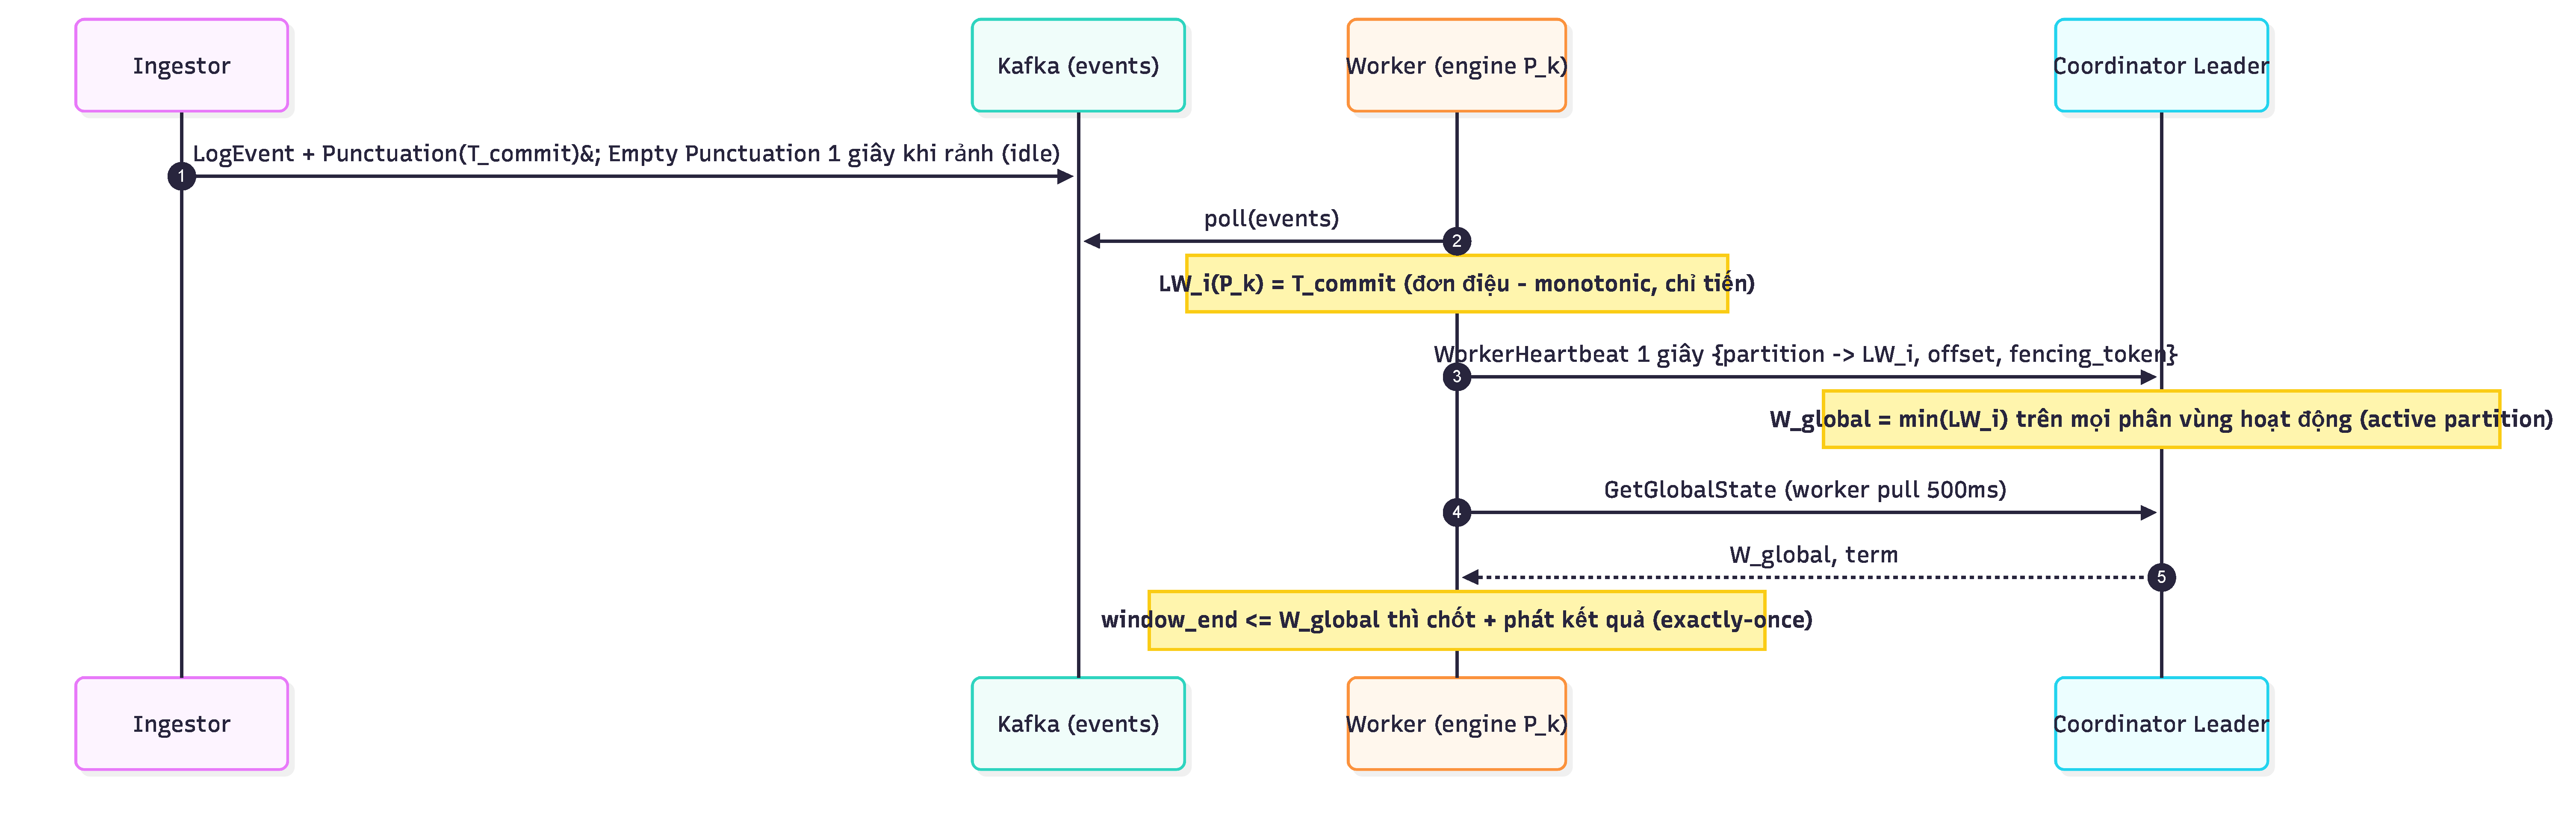
\includegraphics[width=1.15\textwidth]{strict_watermark_seq.pdf}}
    \caption{Sơ đồ}
    \label{fig:strict_watermark_seq}
\end{figure}
\textbf{Liên hệ.} \tcbhighmath{LW_i} bắt nguồn từ Punctuation đi \textit{trong} luồng Kafka (\ref{sec:kafka-pq}); heartbeat mang \tcbhighmath{LW_i} lên Coordinator (\ref{sec:coordinator-aggregator}) qua kênh control out-of-band (\ref{sec:layer-communication}); kết quả và state được bền hóa qua Tiered Storage (\ref{sec:tiered-storage}). So với Heuristic (\ref{sec:heuristic-watermark}), Strict dùng chung mọi chặng — chỉ khác nguồn watermark và control plane.

\subsection{1.2 Phản biện: Vì sao thiết kế như vậy}
Mục Strict phải bảo vệ cam kết "đóng window rồi thì không còn event cũ nào bị bỏ sót". Vì vậy các phương án làm watermark chạy nhanh hơn đều phải bị kiểm tra bằng câu hỏi: có còn chứng minh được dữ liệu đã đủ chưa?
\textbf{Phản đề 1: Không cần Punctuation Token, Worker tự đoán watermark từ event mới nhất.}

\begin{itemize}
\item \textbf{Vì sao nghe hợp lý:} bỏ được cơ chế token, Ingestor đơn giản hơn, watermark có thể tiến nhanh hơn vì Worker không phải chờ mốc xác nhận từ nguồn.
\item \textbf{Lý do bác bỏ:} Worker chỉ nhìn thấy dữ liệu cục bộ của partition mình đang xử lý. Nếu Worker thấy partition \texttt{P0} đã đến event-time 200 nhưng partition \texttt{P7} vẫn còn event-time 150 chưa đến, Worker không có bằng chứng để chốt window toàn cục. Tự đoán watermark biến Strict thành Heuristic trá hình, vì hệ thống đang suy luận từ quan sát cục bộ thay vì nhận cam kết đầy đủ từ nguồn.
\item \textbf{Kết luận phản biện:} Strict bắt buộc cần Punctuation Token. Token là bằng chứng từ Ingestor rằng partition đó đã phát hết event có \tcbhighmath{T_{event} \le T_{commit}}; nhờ vậy window đóng không bỏ sót dữ liệu.
\end{itemize}
\textbf{Phản đề 2: Partition idle nên bị loại khỏi \texttt{min()} để watermark chạy nhanh hơn.}

\begin{itemize}
\item \textbf{Vì sao nghe hợp lý:} một partition lâu không có log sẽ kéo \tcbhighmath{W_{global}} đứng yên; loại nó khỏi \texttt{min()} giúp giảm latency.
\item \textbf{Lý do bác bỏ:} idle không đồng nghĩa với "đã hết dữ liệu cũ". Nếu partition đó gửi log trở lại với event-time nhỏ hơn watermark đã tiến, các log này sẽ bị coi là late dù thực chất chưa từng được xử lý. Khi đó Strict mất cam kết 0\% loss.
\item \textbf{Kết luận phản biện:} Strict không được âm thầm bỏ partition idle. Cách đúng là Empty Punctuation: Ingestor phát token rỗng cho partition rảnh để chứng minh partition đó đã an toàn đến mốc mới.
\end{itemize}

\section{2. Thiết kế Heuristic Watermark}
\label{sec:heuristic-watermark}

\subsection{2.1 Trình bày chi tiết thiết kế}
\textbf{Ý chính.} Heuristic Watermark là thiết kế ưu tiên latency thấp khi upstream không phát được Punctuation Token. Worker không chờ bằng chứng chắc chắn từ nguồn; thay vào đó, mỗi Worker đo độ trễ thực tế của event trong partition mình, đưa mẫu vào DDSketch, lấy \tcbhighmath{L_{eff} = \text{quantile}(0.99)}, rồi đặt \tcbhighmath{W_h = max\_event\_time - L_{eff}}. Aggregator hợp nhất watermark heuristic bằng \tcbhighmath{W_{global\_h} = \min(W_h)}. Bản ghi đến sau khi window đã đóng không bị bỏ thầm, mà được đưa vào DLQ và phát correction sau.
\textbf{Bản đồ thiết kế.}
\textbf{Thành phần và trách nhiệm.}

\begin{itemize}
\item \textbf{HeuristicWorker:} nhận event, đo \tcbhighmath{lateness}, cập nhật engine và gửi watermark heuristic.
\item \textbf{HeuristicWatermarkEngine:} giữ window state, tính \tcbhighmath{W_h}, đóng window sớm theo watermark heuristic.
\item \textbf{DDSketch/Sliding DDSketch:} lưu phân phối \tcbhighmath{lateness} theo partition và trả về quantile như p99.
\item \textbf{Aggregator:} nhận \tcbhighmath{W_h} từ nhiều partition và tính \tcbhighmath{W_{global\_h} = \min(W_h)} trên partition active.
\item \textbf{DLQPipeline:} nhận event đến muộn sau khi window đã đóng.
\item \textbf{CorrectionProtocol:} đọc late event từ DLQ và phát correction cho window result.
\end{itemize}
\textbf{Dữ liệu vào.}

\begin{itemize}
\item \textbf{Event:} bản ghi có \texttt{event\_time}, arrival/processing time và payload.
\item \textbf{Lateness sample:} giá trị \tcbhighmath{arrival\_time - event\_time} đưa vào DDSketch.
\item \textbf{Cấu hình quantile:} ví dụ p99 để lấy \tcbhighmath{L_{eff}}.
\end{itemize}
\textbf{Dữ liệu ra.}

\begin{itemize}
\item \textbf{\tcbhighmath{L_{eff}}:} độ trễ hiệu dụng lấy từ DDSketch.
\item \textbf{\tcbhighmath{W_h}:} watermark heuristic cục bộ của partition.
\item \textbf{\tcbhighmath{W_{global\_h}}:} watermark heuristic toàn cục từ Aggregator.
\item \textbf{Late event:} event thuộc window đã đóng, đi vào DLQ.
\item \textbf{Correction message:} bản sửa kết quả sau khi xử lý late event.
\end{itemize}
\textbf{Trạng thái cần giữ.}

\begin{itemize}
\item \textbf{Sketch buckets:} phân phối \tcbhighmath{lateness} hiện tại.
\item \textbf{Open/closed window:} state của window chưa đóng và đã đóng.
\item \textbf{Late event backlog:} hàng đợi late event chờ correction.
\item \textbf{Cold-start state:} trạng thái trước khi \tcbhighmath{sketch} có đủ mẫu tin cậy.
\item \textbf{Correction id đã xử lý:} tránh phát correction trùng.
\end{itemize}
\textbf{Giao tiếp.}

\begin{itemize}
\item \textbf{Worker -> Aggregator:} gửi \tcbhighmath{W_h} qua gRPC chu kỳ ngắn.
\item \textbf{Worker -> Aggregator/endpoint nhẹ:} kéo \tcbhighmath{W_{global\_h}}.
\item \textbf{Worker -> DLQ:} gửi late event khi event thuộc window đã đóng.
\item \textbf{Correction pipeline -> output:} phát correction message cho window result.
\end{itemize}
\textbf{Đầu ra.}

\begin{itemize}
\item \textbf{Kết quả ban đầu:} window result speculative, ưu tiên latency thấp.
\item \textbf{Kết quả sửa sau:} correction để eventual completeness đạt 100\%.
\end{itemize}
\textbf{Thiết kế DLQ và Correction Pipeline.}
\textbf{Mục tiêu.}

\begin{itemize}
\item \textbf{Không drop late event thầm lặng:} event đến sau khi window đã đóng phải được ghi nhận.
\item \textbf{Giữ kết quả gần real-time:} window vẫn được phép emit sớm theo heuristic watermark.
\item \textbf{Đảm bảo đầy đủ sau cùng:} late event được xử lý thành correction để kết quả cuối cùng hội tụ.
\end{itemize}
\textbf{Khi nào event vào DLQ.}

\begin{itemize}
\item \textbf{Window đã đóng:} event có \texttt{event\_time} thuộc window đã emit speculative.
\item \textbf{Watermark đã vượt window:} \texttt{event\_time} nhỏ hơn hoặc bằng vùng đã được heuristic watermark cho đóng.
\item \textbf{Không còn cập nhật trực tiếp:} engine không mở lại window nóng để tránh phá tính đơn điệu của output ban đầu.
\end{itemize}
\textbf{Payload DLQ.}

\begin{itemize}
\item \textbf{Event gốc:} payload nghiệp vụ để tính lại aggregate.
\item \textbf{\tcbhighmath{window\_id}:} window bị ảnh hưởng bởi late event.
\item \textbf{\tcbhighmath{partition\_id}:} partition phát sinh late event.
\item \textbf{\texttt{event\_time}:} thời điểm sự kiện để xác định cửa sổ.
\item \textbf{\tcbhighmath{arrival\_time}:} thời điểm hệ thống nhận late event.
\item \textbf{\tcbhighmath{original\_result\_version}:} version kết quả đã emit trước đó nếu có.
\item \textbf{\texttt{late\_reason}:} lý do đưa vào DLQ, ví dụ \texttt{ARRIVED\_AFTER\_CLOSE}.
\end{itemize}
\textbf{Correction state.}

\begin{itemize}
\item \textbf{Late backlog:} danh sách late event chưa xử lý.
\item \textbf{Correction id:} idempotency key cho bản sửa, thường ghép từ \tcbhighmath{window\_id} và batch late event.
\item \textbf{Correction version:} version tăng dần của kết quả window sau mỗi lần sửa.
\item \textbf{Processed correction ids:} tập id đã xử lý để tránh phát correction trùng.
\end{itemize}
\textbf{Luồng correction.}

\begin{enumerate}
\item Worker phát hiện event thuộc window đã đóng và ghi event vào DLQ.
\item Correction pipeline đọc DLQ theo batch hoặc theo window.
\item Pipeline tính \tcbhighmath{delta} mà late event tạo ra cho aggregate cũ.
\item Pipeline tạo correction message có \tcbhighmath{window\_id}, \tcbhighmath{delta}, \tcbhighmath{correction\_id} và \tcbhighmath{correction\_version}.
\item Output sink áp dụng correction theo idempotency key.
\item Khi correction ack thành công, pipeline đánh dấu late event/correction là đã xử lý.
\end{enumerate}
\textbf{Thuật toán Heuristic Watermark.}
\textbf{Input của thuật toán.}

\begin{itemize}
\item \textbf{Event hiện tại \tcbhighmath{e}:} gồm \texttt{event\_time}, \tcbhighmath{arrival\_time}, \tcbhighmath{partition\_id} và payload.
\item \textbf{Thời điểm xử lý \tcbhighmath{now}:} thời điểm Worker nhận/xử lý event.
\item \textbf{Quantile cấu hình \tcbhighmath{p}:} ví dụ \tcbhighmath{p = 0.99} để lấy p99 \tcbhighmath{lateness}.
\item \textbf{Window size:} 5 giây.
\item \textbf{Trạng thái partition:} active, idle hoặc cold-start.
\end{itemize}
\textbf{Output của thuật toán.}

\begin{itemize}
\item \textbf{Local heuristic watermark \texttt{\tcbhighmath{W_h}[partition]}:} watermark cục bộ của partition.
\item \textbf{Global heuristic watermark \tcbhighmath{W_{global\_h}}:} watermark toàn cục do Aggregator tính.
\item \textbf{Window result speculative:} kết quả window được emit sớm.
\item \textbf{Late event hoặc correction:} sinh ra khi event đến sau lúc window đã đóng.
\end{itemize}
\textbf{Biến nội bộ tại Worker.}

\begin{itemize}
\item \textbf{\tcbhighmath{max\_event\_time}:} event-time lớn nhất Worker đã thấy trong partition.
\item \textbf{\tcbhighmath{lateness}:} độ trễ của event, tính bằng \tcbhighmath{now - event\_time}.
\item \textbf{\tcbhighmath{sketch}:} DDSketch lưu phân phối \tcbhighmath{lateness} của partition.
\item \textbf{\tcbhighmath{L_{eff}}:} \tcbhighmath{lateness} hiệu dụng lấy từ \texttt{sketch.quantile(}\tcbhighmath{p}\texttt{)}.
\item \textbf{\tcbhighmath{W_{h\_prev}}:} watermark heuristic cục bộ trước đó.
\item \textbf{\tcbhighmath{W_{h\_raw}}:} watermark tạm trước khi áp dụng hysteresis/rate limit.
\item \textbf{\texttt{closed\_windows}:} tập window đã đóng để phát hiện late event.
\end{itemize}
\textbf{Thuật toán tại Worker cho mỗi event (mô tả từng bước).}

\begin{enumerate}
\item \textbf{Đo \tcbhighmath{lateness}:} Worker không đo bằng \tcbhighmath{offset} Kafka, mà đo bằng chênh lệch giữa thời điểm xử lý và \texttt{event\_time}.
\item \textbf{Cập nhật DDSketch:} mỗi \tcbhighmath{lateness} sample làm phân phối \tcbhighmath{lateness} của partition chính xác hơn.
\item \textbf{Cập nhật \tcbhighmath{max\_event\_time}:} Worker nhớ mốc event-time mới nhất đã quan sát để biết dòng dữ liệu đang tiến tới đâu.
\item \textbf{Tính \tcbhighmath{L_{eff}}:} lấy quantile như p99 để chừa một khoảng an toàn cho phần lớn event đến muộn.
\item \textbf{Tạo watermark thô:} \tcbhighmath{W_{h\_raw} = \tcbhighmath{max\_event\_time - L_{eff}}}. Nghĩa là: chỉ đóng đến trước mốc mà thuật toán tin rằng đa số event cũ đã đến.
\item \textbf{Chặn watermark tăng quá nhanh:} rate limit tránh watermark nhảy xa khi vài event mới đẩy \tcbhighmath{max\_event\_time} lên đột ngột.
\item \textbf{Chống dao động nhỏ:} hysteresis tránh việc watermark thay đổi vì nhiễu nhỏ của phân phối \tcbhighmath{lateness}.
\item \textbf{Gửi lên Aggregator:} Worker không tự quyết định toàn cục; nó chỉ gửi watermark cục bộ của partition.
\end{enumerate}
\textbf{Thuật toán tại Aggregator (mô tả từng bước).}

\begin{enumerate}
\item \textbf{Nhận watermark cục bộ:} mỗi Worker gửi \tcbhighmath{W_h} theo partition.
\item \textbf{Lọc partition idle:} Heuristic loại partition thật sự idle để một partition rảnh không treo \texttt{min()} mãi.
\item \textbf{Lấy min trên partition active:} \texttt{min()} vẫn cần thiết vì window toàn cục chỉ nên đóng đến mốc an toàn nhất trong các partition đang có dữ liệu.
\item \textbf{Giữ đơn điệu:} \tcbhighmath{W_{global\_h} = \max(W_{global\_h\_prev}, W_{candidate})} để watermark toàn cục không tụt lùi.
\item \textbf{Trả watermark cho Worker:} Worker dùng \tcbhighmath{W_{global\_h}} để quyết định window nào được đóng.
\end{enumerate}
\textbf{Điều kiện đóng window.} Window được đóng khi cuối window nhỏ hơn hoặc bằng \tcbhighmath{W_{global\_h}}. Vì watermark này là heuristic, kết quả được xem là speculative: nhanh, nhưng có thể cần correction nếu late event xuất hiện.
\textbf{Điều kiện đưa event vào DLQ.} Event vào DLQ không có nghĩa là bị mất. Nó được giữ lại để correction pipeline tính \tcbhighmath{delta} và phát bản sửa cho window đã emit.
\textbf{Ví dụ vận hành và thuật toán.}

\begin{itemize}
\item \textbf{Cấu hình hệ thống:} Độ phân vị \tcbhighmath{p = 0.99}, kích thước cửa sổ 5 giây.
\item \textbf{Bước 1 (Worker đo \tcbhighmath{lateness} cục bộ):} Tại partition \texttt{P0}, Worker nhận các bản ghi log và đo độ trễ thực tế. \tcbhighmath{max\_event\_time = 200s}. Phác họa \tcbhighmath{sketch} thống kê và trả về phân vị 99\% của độ trễ là \tcbhighmath{L_{eff} = 4s}.
\item \textbf{Bước 2 (Tính watermark cục bộ):} \tcbhighmath{W_h = max\_event\_time - L_{eff} = 200s - 4s = 196s}.
\item \textbf{Bước 3 (Aggregator tổng hợp):} Aggregator nhận báo cáo từ các partition đang hoạt động: \texttt{P0 = 196s}, \texttt{P1 = 198s}, \texttt{P2 = 194s}. Aggregator tính \tcbhighmath{W_{global\_h} = \min(196, 198, 194) = 194s}.
\item \textbf{Bước 4 (Đóng window speculative):} Worker nhận \tcbhighmath{W_{global\_h} = 194s}. Cửa sổ \texttt{[185, 190)} có \texttt{\tcbhighmath{window\_end} = 190 <= 194s} được đóng và phát kết quả tạm tính (speculative result).
\item \textbf{Bước 5 (Xử lý sự kiện đến muộn qua DLQ):} Một event có \texttt{event\_time = 192s} (thuộc cửa sổ \texttt{[190, 195)}) đến muộn khi \texttt{\tcbhighmath{now} = 206s} (\tcbhighmath{lateness} = 14s). Lúc này watermark toàn cục đã vượt qua \texttt{192s}, cửa sổ đã đóng. Bản ghi này được phát hiện là late event, tự động được gửi vào DLQ để pipeline hiệu chỉnh tính toán lại và phát \texttt{Correction Message} sửa đổi kết quả cửa sổ \texttt{[190, 195)}.
\end{itemize}
\textbf{Cách chạy từng bước.}

\begin{enumerate}
\item Khi event đến Worker, engine tính \tcbhighmath{lateness} của event bằng chênh lệch giữa thời điểm xử lý và \texttt{event\_time}. Mẫu \tcbhighmath{lateness} này được đưa vào DDSketch của partition.
\item DDSketch giữ phân phối \tcbhighmath{lateness} theo thang log, nên vẫn mô tả được cả event đến gần như đúng giờ lẫn event trễ rất dài mà không cần histogram khổng lồ.
\item Sau giai đoạn warm-up, engine lấy phân vị cấu hình, ví dụ p99, để tạo \tcbhighmath{L_{eff}}. Watermark cục bộ được tính theo \tcbhighmath{W_h = max\_event\_time - L_{eff}}, rồi bị chặn bởi hysteresis/rate limit để không nhảy quá gắt.
\item Aggregator nhận \tcbhighmath{W_h} từ nhiều partition, bỏ qua partition thật sự idle theo rule của Heuristic, và tính \tcbhighmath{W_{global\_h} = \min(W_h)} trên phần còn active.
\item Worker đóng window theo \tcbhighmath{W_{global\_h}}. Vì đây là watermark dự đoán, kết quả đầu tiên là kết quả speculative. Nếu sau đó có event thuộc window đã đóng, event được đưa vào DLQ cùng \tcbhighmath{window\_id}, payload gốc và thông tin correction.
\item Correction pipeline đọc DLQ, tính phần chênh lệch cần cộng/trừ vào window result, rồi phát correction để kết quả sau cùng vẫn đầy đủ.
\end{enumerate}

\begin{figure}[H]
    \centering
    \makebox[\textwidth][c]{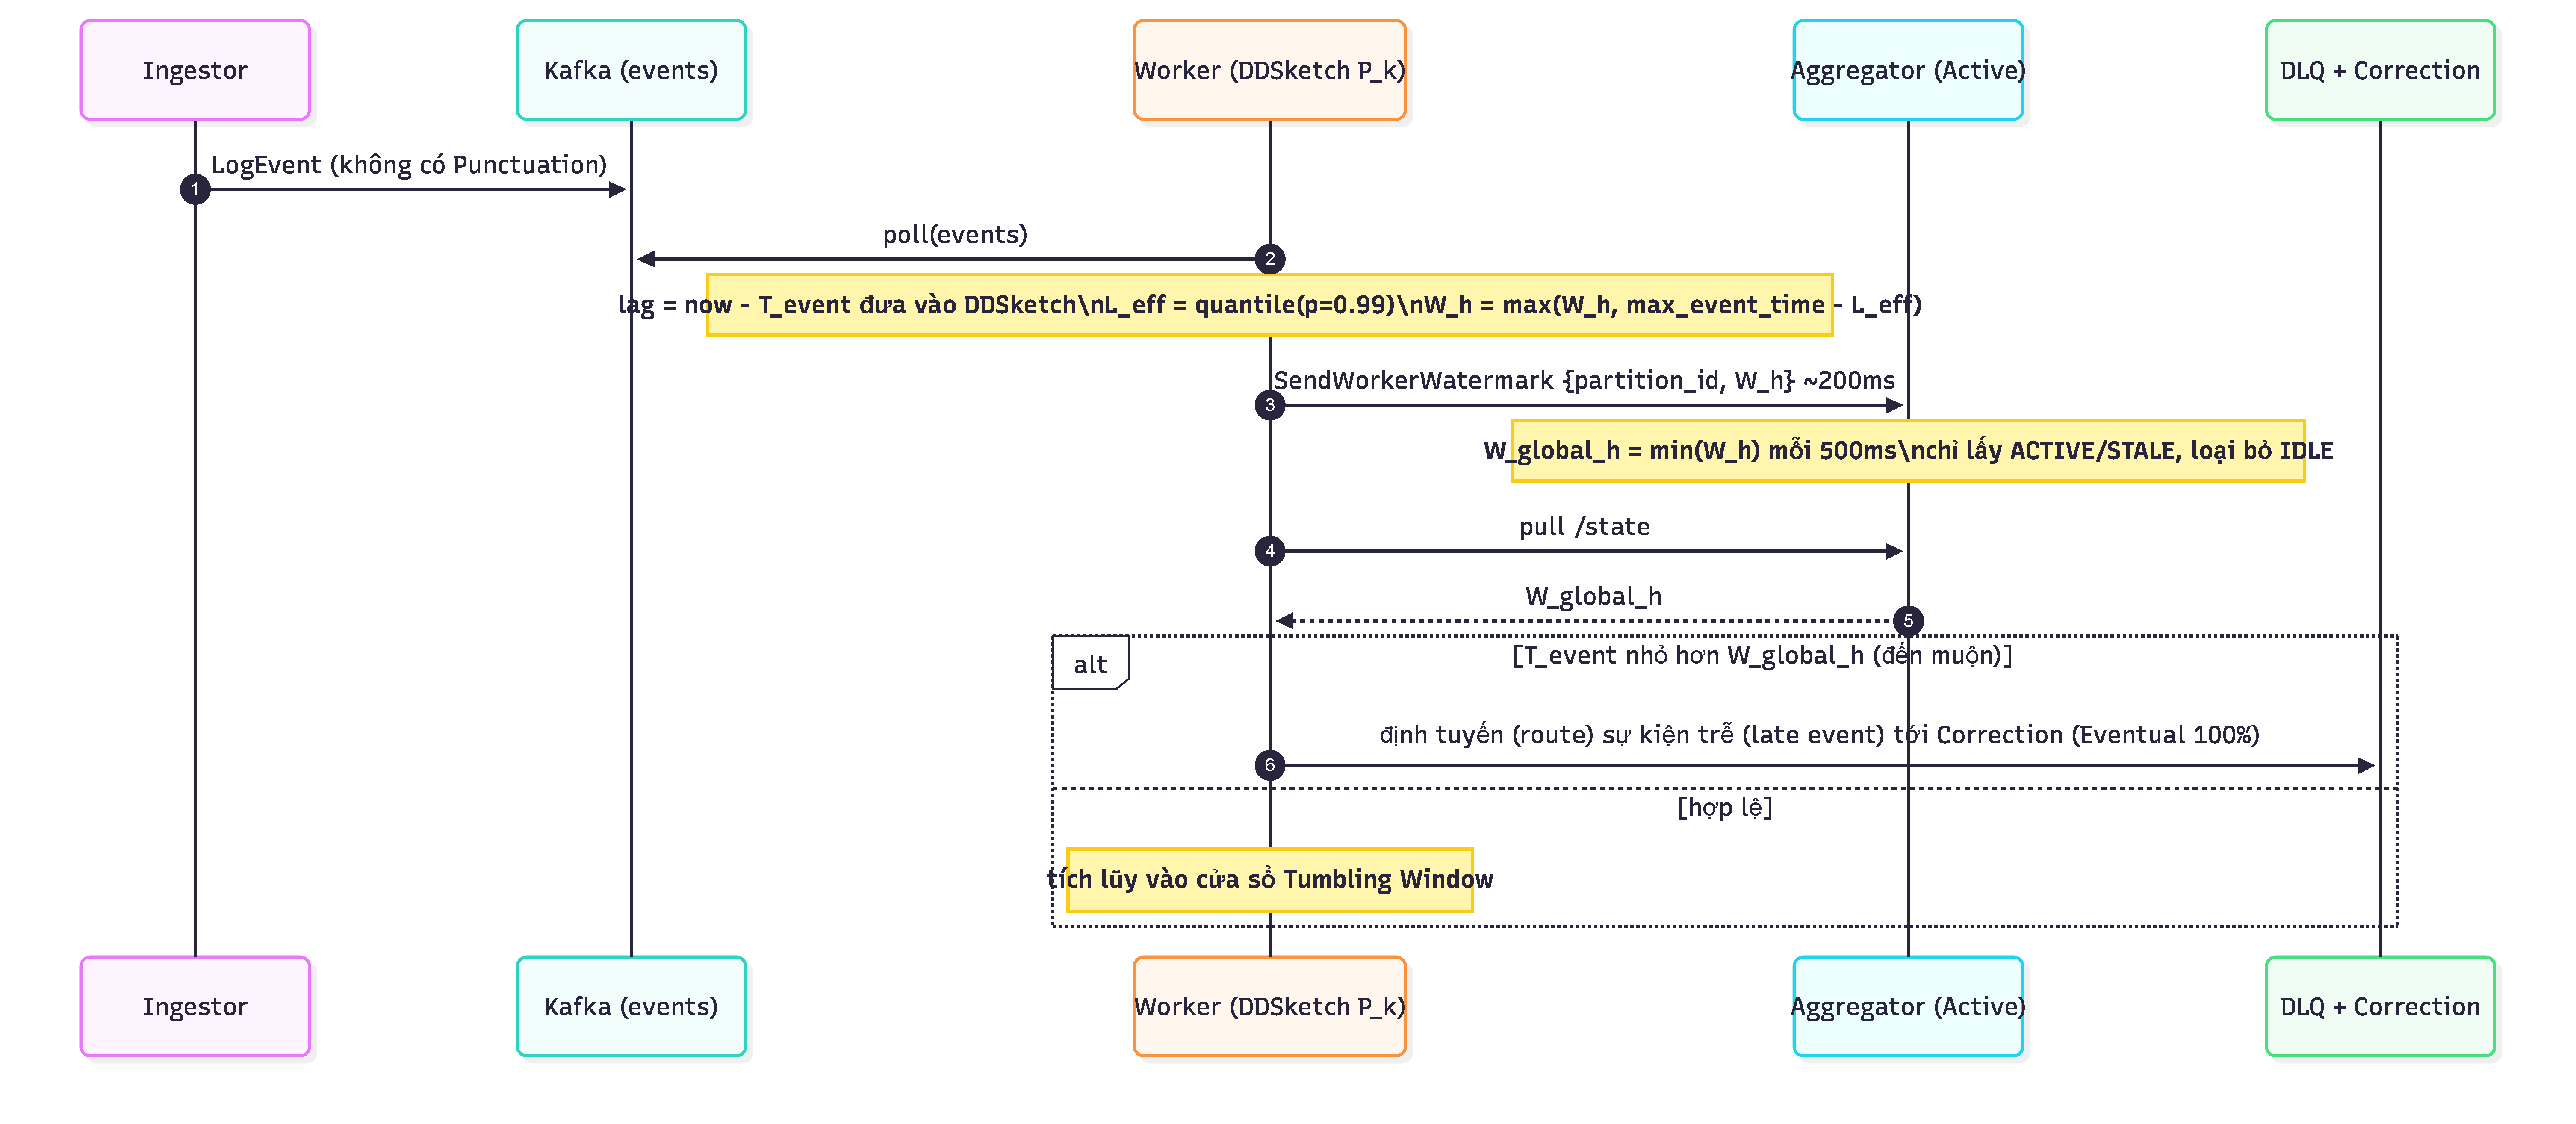
\includegraphics[width=1.15\textwidth]{heuristic_watermark_seq.pdf}}
    \caption{Sơ đồ}
    \label{fig:heuristic_watermark_seq}
\end{figure}
\textbf{Liên hệ.} Heuristic tái dùng đúng đường dữ liệu của Strict — Kafka + Bounded PQ (\ref{sec:kafka-pq}), engine theo partition (\ref{sec:node-partition}), Tiered Storage (\ref{sec:tiered-storage}) — chỉ thay nguồn watermark (DDSketch thay token \ref{sec:strict-watermark}), đổi control plane sang Aggregator (\ref{sec:coordinator-aggregator}) và thêm nhánh DLQ. Late event vào DLQ chính là phần Strict (\ref{sec:strict-watermark}) không có.

\subsection{2.2 Phản biện: Vì sao thiết kế như vậy}
Mục Heuristic không cố chứng minh "không bao giờ có late event". Nó chọn latency thấp, nhưng phải nói rõ sai số được đo, được giới hạn và được sửa bằng DLQ/correction.
\textbf{Phản đề 1: Dùng EWMA hoặc histogram cố định thay DDSketch cho đơn giản.}

\begin{itemize}
\item \textbf{Vì sao nghe hợp lý:} EWMA dễ cài, histogram cố định dễ giải thích, cả hai đều có thể mô tả độ trễ trung bình của luồng log.
\item \textbf{Lý do bác bỏ:} watermark không cần trung bình, mà cần tail \tcbhighmath{lateness} như p95/p99 để biết nên chừa bao nhiêu thời gian cho event muộn. EWMA che mất tail; histogram cố định khó chọn bucket vì \tcbhighmath{lateness} có thể trải qua nhiều bậc độ lớn; Aggregator còn cần merge phân phối từ nhiều partition mà không làm mất ý nghĩa phân vị.
\item \textbf{Kết luận phản biện:} DDSketch phù hợp hơn vì giữ phân vị với sai số tương đối, merge được giữa partition và dùng bộ nhớ giới hạn.
\end{itemize}
\textbf{Phản đề 2: Nếu sợ sai thì cứ chờ đủ, không cần Heuristic.}

\begin{itemize}
\item \textbf{Vì sao nghe hợp lý:} chờ lâu hơn sẽ giảm late event và tránh phải có correction pipeline.
\item \textbf{Lý do bác bỏ:} chờ đủ chính là mục tiêu của Strict, nhưng Heuristic được thiết kế cho trường hợp upstream không phát token hoặc SLA yêu cầu latency thấp hơn. Nếu cứ chờ như Strict, mode Heuristic mất lý do tồn tại.
\item \textbf{Kết luận phản biện:} Heuristic được phép chốt sớm, nhưng phải đi kèm DLQ và Correction để late event không bị mất thầm lặng.
\end{itemize}
\textbf{Phản đề 3: Partition IDLE vẫn nên nằm trong \texttt{min()} giống Strict.}

\begin{itemize}
\item \textbf{Vì sao nghe hợp lý:} giữ partition idle trong \texttt{min()} có vẻ an toàn hơn vì không bỏ qua nguồn dữ liệu nào.
\item \textbf{Lý do bác bỏ:} Heuristic không có Empty Punctuation để chứng minh partition idle đã an toàn. Nếu giữ partition rảnh trong \texttt{min()}, watermark heuristic có thể bị treo vô hạn dù các partition còn lại vẫn có dữ liệu mới.
\item \textbf{Kết luận phản biện:} Heuristic loại partition thật sự idle khỏi \texttt{min()} để giữ latency, còn rủi ro late event được hấp thụ bằng DLQ và correction.
\end{itemize}

\section{3. Thiết kế Node quản lý Partition}
\label{sec:node-partition}

\subsection{3.1 Trình bày chi tiết thiết kế}
\textbf{Ý chính.} Worker Node là nơi chạy xử lý thực tế, nhưng đơn vị quản lý đúng không phải là node mà là partition. Một Worker có thể giữ nhiều partition, ví dụ 3 partition trên một node, nhưng mỗi partition có engine, buffer, state và watermark riêng. Khi gửi heartbeat, Worker gửi bản đồ watermark từng partition thay vì tự gộp thành một watermark của node.
\textbf{Bản đồ thiết kế.}
\textbf{Thành phần và trách nhiệm.}

\begin{itemize}
\item \textbf{Worker process:} tiến trình chạy nhiều partition trên cùng node.
\item \textbf{Partition assignment:} danh sách partition mà Worker đang sở hữu.
\item \textbf{Map \texttt{\tcbhighmath{partition\_id} -> engine}:} mỗi partition trỏ đến engine xử lý riêng.
\item \textbf{Map \texttt{\tcbhighmath{partition\_id} -> buffer}:} mỗi partition có buffer event-time riêng.
\item \textbf{Lock theo partition:} bảo vệ thao tác flush/pause/reassign của từng partition.
\item \textbf{RocksDB/checkpoint theo partition:} lưu state và \tcbhighmath{offset} tách biệt để bàn giao độc lập.
\end{itemize}
\textbf{Dữ liệu vào.}

\begin{itemize}
\item \textbf{Batch event từ Kafka:} batch chứa record thuộc một hoặc nhiều partition.
\item \textbf{Partition id:} khóa để dispatch record vào đúng buffer/engine.
\item \textbf{Lệnh control:} pause, resume, reassign, flush khi failover/failback.
\end{itemize}
\textbf{Dữ liệu ra.}

\begin{itemize}
\item \textbf{Local watermark từng partition:} \tcbhighmath{LW_i} trong Strict hoặc \tcbhighmath{W_h} trong Heuristic.
\item \textbf{Metric queue/backpressure:} queue size, pause/resume status, lag.
\item \textbf{Heartbeat per-partition:} trạng thái từng partition gửi lên control plane.
\end{itemize}
\textbf{Trạng thái cần giữ.}

\begin{itemize}
\item \textbf{Owner partition:} Worker nào đang sở hữu partition.
\item \textbf{Buffer event-time:} event đang chờ sắp/xử lý của từng partition.
\item \textbf{Engine state:} open window, aggregate, watermark cục bộ.
\item \textbf{Backpressure flag:} trạng thái pause/resume consume.
\item \textbf{Last event time:} dùng để nhận diện partition idle.
\end{itemize}
\textbf{Giao tiếp.}

\begin{itemize}
\item \textbf{Worker -> Kafka:} poll event theo partition được assign.
\item \textbf{Partition engine -> Worker:} trả watermark/metric cục bộ.
\item \textbf{Worker -> Coordinator/Aggregator:} gửi heartbeat dạng map theo partition.
\item \textbf{Control plane -> Worker:} gửi lệnh pause, flush, reassign hoặc resume.
\end{itemize}
\textbf{Đầu ra.}

\begin{itemize}
\item \textbf{Heartbeat chi tiết:} trạng thái từng partition, không phải trạng thái gộp của node.
\item \textbf{Window result:} kết quả sinh từ engine của từng partition.
\end{itemize}
\textbf{Cách chạy từng bước.}

\begin{enumerate}
\item Coordinator gán một tập partition cho Worker. Worker tạo engine, buffer, lock và state store riêng cho từng partition trong tập đó.
\item Khi poll được batch từ Kafka, Worker nhìn \tcbhighmath{partition\_id} của từng record để dispatch vào đúng buffer. Event của partition \texttt{P3} không được đi vào engine của \texttt{P4}, dù hai partition đang nằm trên cùng một process Worker.
\item Mỗi partition xử lý độc lập: buffer sắp event, engine cập nhật window, local watermark tăng theo mode Strict hoặc Heuristic, checkpoint ghi theo partition.
\item Heartbeat của Worker là một map chi tiết, ví dụ \texttt{{P0: watermark/\tcbhighmath{offset}/status, P1: watermark/\tcbhighmath{offset}/status, P2: watermark/\tcbhighmath{offset}/status}}. Control plane nhìn được partition nào chậm, partition nào idle, partition nào cần chuyển chủ.
\item Khi một partition được reassign, Worker chỉ pause/flush/close state của partition đó. Các partition khác trên cùng node vẫn có thể tiếp tục chạy, miễn không dùng chung lock hoặc RocksDB instance gây kẹt.
\end{enumerate}
\textbf{Ví dụ vận hành.}

\begin{itemize}
\item \textbf{Bố trí ban đầu:} Hệ thống gồm 2 Worker: \texttt{W1} (gánh \texttt{P0}, \texttt{P1}, \texttt{P2}) và \texttt{W2} (gánh \texttt{P3}, \texttt{P4}, \texttt{P5}).
\item \textbf{Trường hợp 1 (Nhiều partition độc lập trên cùng node):} Partition \texttt{P1} trên \texttt{W1} bị nghẽn (do Kafka partition \texttt{P1} có burst lượng log lớn), khiến local watermark của \texttt{P1} đứng yên tại 100. Các partition \texttt{P0} và \texttt{P2} trên \texttt{W1} vẫn chạy mượt và tăng local watermark lên 120. Nhờ heartbeat báo cáo chi tiết dạng map \texttt{{P0: 120, P1: 100, P2: 120}}, Coordinator biết chính xác chỉ \texttt{P1} bị chậm, \texttt{P0} và \texttt{P2} vẫn bình thường.
\item \textbf{Trường hợp 2 (Failover cô lập):} Nếu \texttt{P1} trên \texttt{W1} bị lỗi nghiêm trọng về RocksDB local, Coordinator chỉ cần thực hiện failover chuyển quyền sở hữu riêng partition \texttt{P1} sang \texttt{W2}. Tiến trình \texttt{W1} không bị khởi động lại hay tạm dừng toàn bộ; các partition \texttt{P0} và \texttt{P2} trên \texttt{W1} tiếp tục tiêu thụ dữ liệu và cập nhật bình thường mà không bị ảnh hưởng.
\end{itemize}

\begin{figure}[H]
    \centering
    \makebox[\textwidth][c]{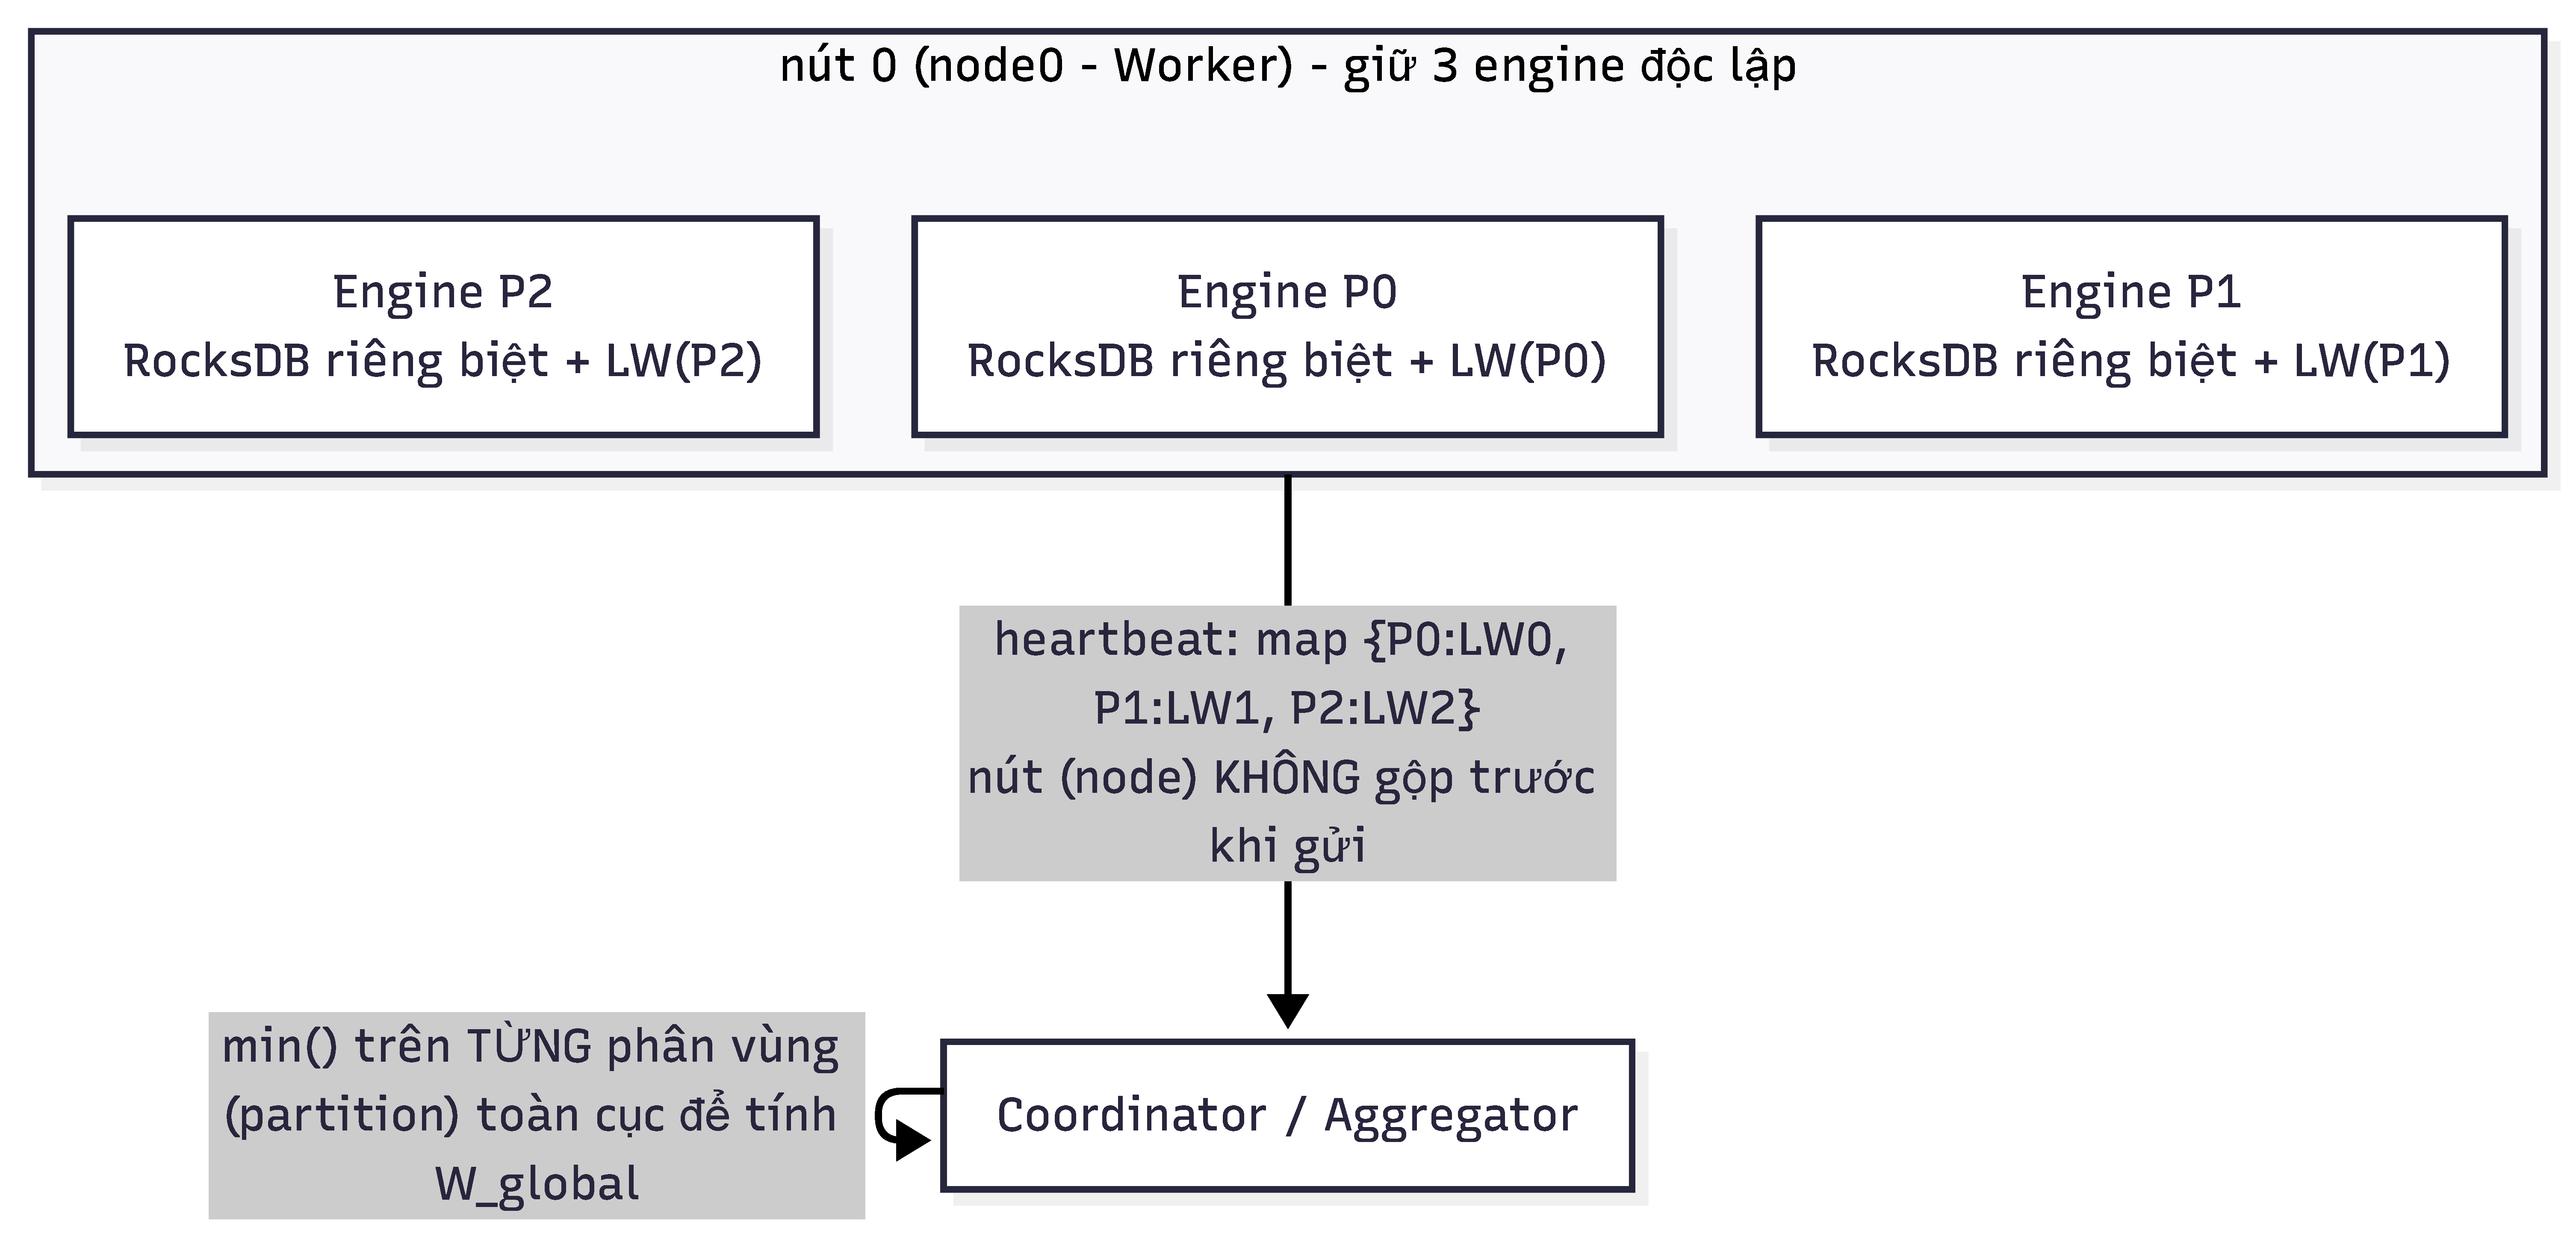
\includegraphics[width=1.15\textwidth]{node_partition_engine.pdf}}
    \caption{Sơ đồ}
    \label{fig:node_partition_engine}
\end{figure}
\textbf{Liên hệ.} Watermark mà mỗi engine sinh ra (\ref{sec:strict-watermark} \tcbhighmath{LW_i} / \ref{sec:heuristic-watermark} \tcbhighmath{W_h}) được node gom thành \textit{map} rồi gửi control plane (\ref{sec:coordinator-aggregator}) qua kênh control (\ref{sec:layer-communication}). Vì đơn vị là partition nên khi node chết, chỉ partition đó được bàn giao qua Failback (\ref{sec:failback-5step}) dựa trên checkpoint per-partition (\ref{sec:tiered-storage}).

\subsection{3.2 Phản biện: Vì sao thiết kế như vậy}
Mục Worker/Partition phải bảo vệ nguyên tắc: partition là đơn vị sở hữu, xử lý, checkpoint và failover. Node chỉ là nơi đang chạy partition ở thời điểm hiện tại.
\textbf{Phản đề 1: Một Worker dùng chung một engine và một RocksDB cho mọi partition.}

\begin{itemize}
\item \textbf{Vì sao nghe hợp lý:} ít object hơn, ít thư mục RocksDB hơn, code quản lý state có vẻ gọn hơn.
\item \textbf{Lý do bác bỏ:} khi failover chỉ một partition, hệ thống cần flush, đóng khóa, checkpoint và bàn giao đúng partition đó. Nếu nhiều partition dùng chung engine/state store, việc chuyển riêng một partition sẽ kéo theo state của partition khác, dễ tranh chấp lock và khó xác định \tcbhighmath{offset} an toàn theo partition.
\item \textbf{Kết luận phản biện:} mỗi partition cần engine, buffer, lock và state riêng để có thể chuyển giao độc lập mà không dừng cả node.
\end{itemize}
\textbf{Phản đề 2: Worker gộp watermark theo node rồi mới gửi lên control plane.}

\begin{itemize}
\item \textbf{Vì sao nghe hợp lý:} heartbeat nhỏ hơn, Coordinator/Aggregator xử lý ít key hơn, nhìn bề ngoài hệ thống đơn giản hơn.
\item \textbf{Lý do bác bỏ:} watermark theo node che mất khác biệt giữa các partition. Một partition chậm sẽ kéo lùi oan các partition khỏe; ngược lại, nếu gộp không cẩn thận, partition chậm có thể bị che khuất và gây late/loss. Control plane cũng không biết partition nào cần failover hoặc đang idle.
\item \textbf{Kết luận phản biện:} heartbeat phải giữ map theo partition. Gộp theo node chỉ nên dùng cho metric tổng hợp, không dùng cho quyết định watermark và ownership.
\end{itemize}

\section{4. Thiết kế Kafka + Bounded Priority Queue tại Node}
\label{sec:kafka-pq}

\subsection{4.1 Trình bày chi tiết thiết kế}
\textbf{Ý chính.} Kafka là data plane bền vững của hệ thống. Event được ghi vào Kafka theo partition và \tcbhighmath{offset} để Worker có thể đọc lại sau sự cố. Tuy nhiên Kafka chỉ giữ thứ tự append theo \tcbhighmath{offset} trong partition, không sắp xếp lại theo event-time. Vì vậy mỗi Worker đặt thêm một BoundedPriorityQueue, triển khai như min-heap theo event-time, ở phía client trước khi event đi vào window engine.
\textbf{Bản đồ thiết kế.}
\textbf{Thành phần và trách nhiệm.}

\begin{itemize}
\item \textbf{Ingestor/KafkaProducer:} ghi event vào Kafka theo key/partition.
\item \textbf{Kafka topic \texttt{events}:} lưu event bền vững theo partition và \tcbhighmath{offset}.
\item \textbf{Kafka consumer ở Worker:} poll batch event theo partition được assign.
\item \textbf{BoundedPriorityQueue:} min-heap giới hạn kích thước/thời gian, sắp event theo event-time.
\item \textbf{Window engine:} nhận event đã qua queue và cập nhật window state.
\end{itemize}
\textbf{Quan hệ giữa Kafka, Worker node và partition.}
Trong thiết kế này cần phân biệt rõ \textbf{Kafka partition} và \textbf{partition xử lý do node quản lý}. Hai khái niệm này dùng cùng một \tcbhighmath{partition\_id}, nhưng trách nhiệm khác nhau:

\begin{table}[H]
\centering
\begin{tabular}{p{2.5cm}p{2.2cm}p{2.2cm}p{2.2cm}p{5.5cm}}
\toprule
\textbf{Thành phần} & \textbf{Nằm ở đâu} & \textbf{Gắn với node không?} & \textbf{Gắn với partition không?} & \textbf{Vai trò trong thiết kế} \\
\midrule
Kafka topic \texttt{events} & Kafka broker & Không gắn cố định với Worker node & Có, theo Kafka partition & Lưu log event bền vững theo \tcbhighmath{offset} \\
Worker node & Cụm xử lý & Có, là process/máy đang chạy & Có, nhận một tập partition được giao & Đọc event, sắp event-time, cập nhật state \\
Consumer assignment & Coordinator/consumer group & Có, xác định node nào đang xử lý & Có, assign theo partition & Ràng buộc \tcbhighmath{partition\_id} -> \tcbhighmath{worker\_id} tại thời điểm hiện tại \\
Kafka \tcbhighmath{offset}/checkpoint & Kafka + Tier-2 checkpoint & Không nên gắn vĩnh viễn với node & Có, \tcbhighmath{offset} luôn theo topic-partition & Biết replay từ đâu khi recovery/failover \\
BoundedPriorityQueue và window engine & Bộ nhớ/state local của Worker & Có, nằm trên owner node hiện tại & Có, tách riêng theo partition & Sắp out-of-order và xử lý window cho partition đó \\
\bottomrule
\end{tabular}
\end{table}
Ví dụ topic \texttt{events} có 12 partition \texttt{P0..P11} và có 4 Worker node \texttt{W1..W4}. Coordinator có thể gán:

\begin{itemize}
\item \texttt{W1} quản lý \texttt{P0}, \texttt{P1}, \texttt{P2}.
\item \texttt{W2} quản lý \texttt{P3}, \texttt{P4}, \texttt{P5}.
\item \texttt{W3} quản lý \texttt{P6}, \texttt{P7}, \texttt{P8}.
\item \texttt{W4} quản lý \texttt{P9}, \texttt{P10}, \texttt{P11}.
\end{itemize}
Kafka vẫn là nơi lưu toàn bộ log của \texttt{P0..P11}. Worker node không sở hữu dữ liệu Kafka; Worker chỉ là \textbf{consumer/processor owner} của những partition được giao. Khi nói \texttt{W2} quản lý \texttt{P4}, nghĩa là tại thời điểm đó \texttt{W2} là node duy nhất được phép consume, buffer, tính watermark, cập nhật window state và checkpoint \tcbhighmath{offset} cho \texttt{P4}.
Luồng quan hệ cụ thể như sau:

\begin{enumerate}
\item Ingestor ghi event vào Kafka topic \texttt{events} với key/partition phù hợp. Kafka đặt record vào đúng Kafka partition, ví dụ \texttt{P4}, và cấp \tcbhighmath{offset} tăng dần trong \texttt{P4}.
\item Coordinator hoặc cơ chế consumer assignment biết \texttt{P4} đang thuộc \texttt{W2}, nên chỉ \texttt{W2} được poll record của \texttt{P4}.
\item Bên trong \texttt{W2}, record của \texttt{P4} không đi vào hàng đợi chung của cả node. Nó được đưa vào BoundedPriorityQueue riêng của \texttt{P4}, sau đó đi vào window engine/state riêng của \texttt{P4}.
\item Sau khi xử lý an toàn, \texttt{W2} ghi checkpoint cho \texttt{P4}, gồm Kafka \tcbhighmath{offset} đã xử lý, watermark, window state và metadata cần phục hồi.
\item Nếu \texttt{W2} lỗi và \texttt{P4} chuyển sang \texttt{W1}, \texttt{W1} không đọc state theo tên \texttt{W2}. \texttt{W1} đọc checkpoint theo \texttt{\tcbhighmath{partition\_id}=P4}, khôi phục PQ/state cần thiết, rồi \texttt{seek} Kafka partition \texttt{P4} từ \tcbhighmath{offset} an toàn kế tiếp.
\end{enumerate}
\textbf{Dữ liệu vào.}

\begin{itemize}
\item \textbf{Event key/partition:} xác định event thuộc partition nào.
\item \textbf{Kafka \tcbhighmath{offset}:} vị trí bền vững để replay khi recovery.
\item \textbf{Event-time:} thời điểm sự kiện dùng để sắp heap và tính window.
\item \textbf{Poll batch:} nhóm record Worker lấy từ Kafka.
\end{itemize}
\textbf{Dữ liệu ra.}

\begin{itemize}
\item \textbf{Phần tử heap:} tuple \texttt{(event\_time, counter, event)}.
\item \textbf{Event đã pop:} event được đưa sang engine theo thứ tự event-time tương đối.
\item \textbf{Offset đã checkpoint:} \tcbhighmath{offset} an toàn sau khi event được xử lý.
\end{itemize}
\textbf{Trạng thái cần giữ.}

\begin{itemize}
\item \textbf{Kafka \tcbhighmath{offset} hiện tại:} \tcbhighmath{offset} đã poll và \tcbhighmath{offset} đã checkpoint.
\item \textbf{Heap buffer:} event đang chờ sắp/xả.
\item \textbf{Queue size:} số event trong heap để quyết định backpressure.
\item \textbf{Backpressure pause/resume:} trạng thái tạm dừng hoặc tiếp tục consume Kafka.
\end{itemize}
\textbf{Giao tiếp.}

\begin{itemize}
\item \textbf{Ingestor -> Kafka:} produce event.
\item \textbf{Worker -> Kafka:} poll event và pause/resume consumer khi cần.
\item \textbf{Queue -> Engine:} pop event nhỏ nhất theo event-time sang window engine.
\item \textbf{Engine -> Checkpoint:} ghi \tcbhighmath{offset}/state sau khi xử lý.
\end{itemize}
\textbf{Đầu ra.}

\begin{itemize}
\item \textbf{Event vào engine:} đã được sắp tương đối theo event-time.
\item \textbf{Tín hiệu backpressure:} giúp Worker không tràn RAM khi event đến nhanh hơn tốc độ xử lý.
\end{itemize}
\textbf{Cách chạy từng bước.}

\begin{enumerate}
\item Ingestor ghi event vào Kafka topic \texttt{events}, key theo partition để các event cùng partition giữ thứ tự \tcbhighmath{offset} và có thể replay.
\item Worker consumer poll batch theo partition. Record mới poll chưa được đưa thẳng vào window engine, mà được đưa vào BoundedPriorityQueue.
\item Queue là min-heap theo \texttt{event\_time}, có thêm counter để phá hòa khi hai event cùng timestamp. Nhờ vậy, nếu Kafka đưa ra \tcbhighmath{offset} theo thứ tự \texttt{event\_time=100, 95, 98}, Worker có thể xử lý theo thứ tự gần đúng \texttt{95, 98, 100}.
\item Queue bị giới hạn bởi \texttt{maxsize} và \tcbhighmath{max\_wait\_ms}. Khi queue đầy, phần tử nhỏ nhất được pop sang engine để giải phóng RAM. Khi event nằm trong queue quá lâu, nó cũng được xả để tránh chờ vô hạn.
\item Nếu queue thường xuyên đầy, Worker pause Kafka consumer tạm thời. Kafka giữ log trên broker, còn Worker xử lý bớt heap và resume sau. Offset chỉ nên được xem là an toàn khi event tương ứng đã đi qua engine và state/\tcbhighmath{offset} đã được checkpoint.
\end{enumerate}
\textbf{Ví dụ vận hành.}

\begin{itemize}
\item \textbf{Luồng dữ liệu out-of-order:} Kafka partition \texttt{P4} nhận được 3 event theo thứ tự \tcbhighmath{offset} như sau:
\item Offset 10 mang \texttt{event\_time = 12:00:10}
\item Offset 11 mang \texttt{event\_time = 12:00:02}
\item Offset 12 mang \texttt{event\_time = 12:00:05}
\item \textbf{Bước 1 (Poll dữ liệu):} Worker poll batch này từ Kafka broker.
\item \textbf{Bước 2 (Đưa vào Bounded PQ):} Thay vì xử lý trực tiếp, Worker đẩy cả 3 event vào \texttt{BoundedPriorityQueue} riêng của \texttt{P4}. Queue sắp xếp chúng lại theo thứ tự thời gian sự kiện tăng dần (min-heap).
\item \textbf{Bước 3 (Xả dữ liệu sắp xếp):} Khi queue đạt điều kiện xả (hoặc đầy hoặc hết thời gian chờ), các event được pop ra theo thứ tự: \texttt{12:00:02} (Offset 11) trước, rồi đến \texttt{12:00:05} (Offset 12), cuối cùng mới là \texttt{12:00:10} (Offset 10).
\item \textbf{Bước 4 (Kết quả):} Window engine nhận được luồng event đã được sắp xếp lại gần như tuần tự hoàn hảo theo \tcbhighmath{T_{event}}, giúp watermark của \texttt{P4} không bị nhảy giật cục bộ và tránh đóng nhầm cửa sổ.
\end{itemize}

\begin{figure}[H]
    \centering
    \makebox[\textwidth][c]{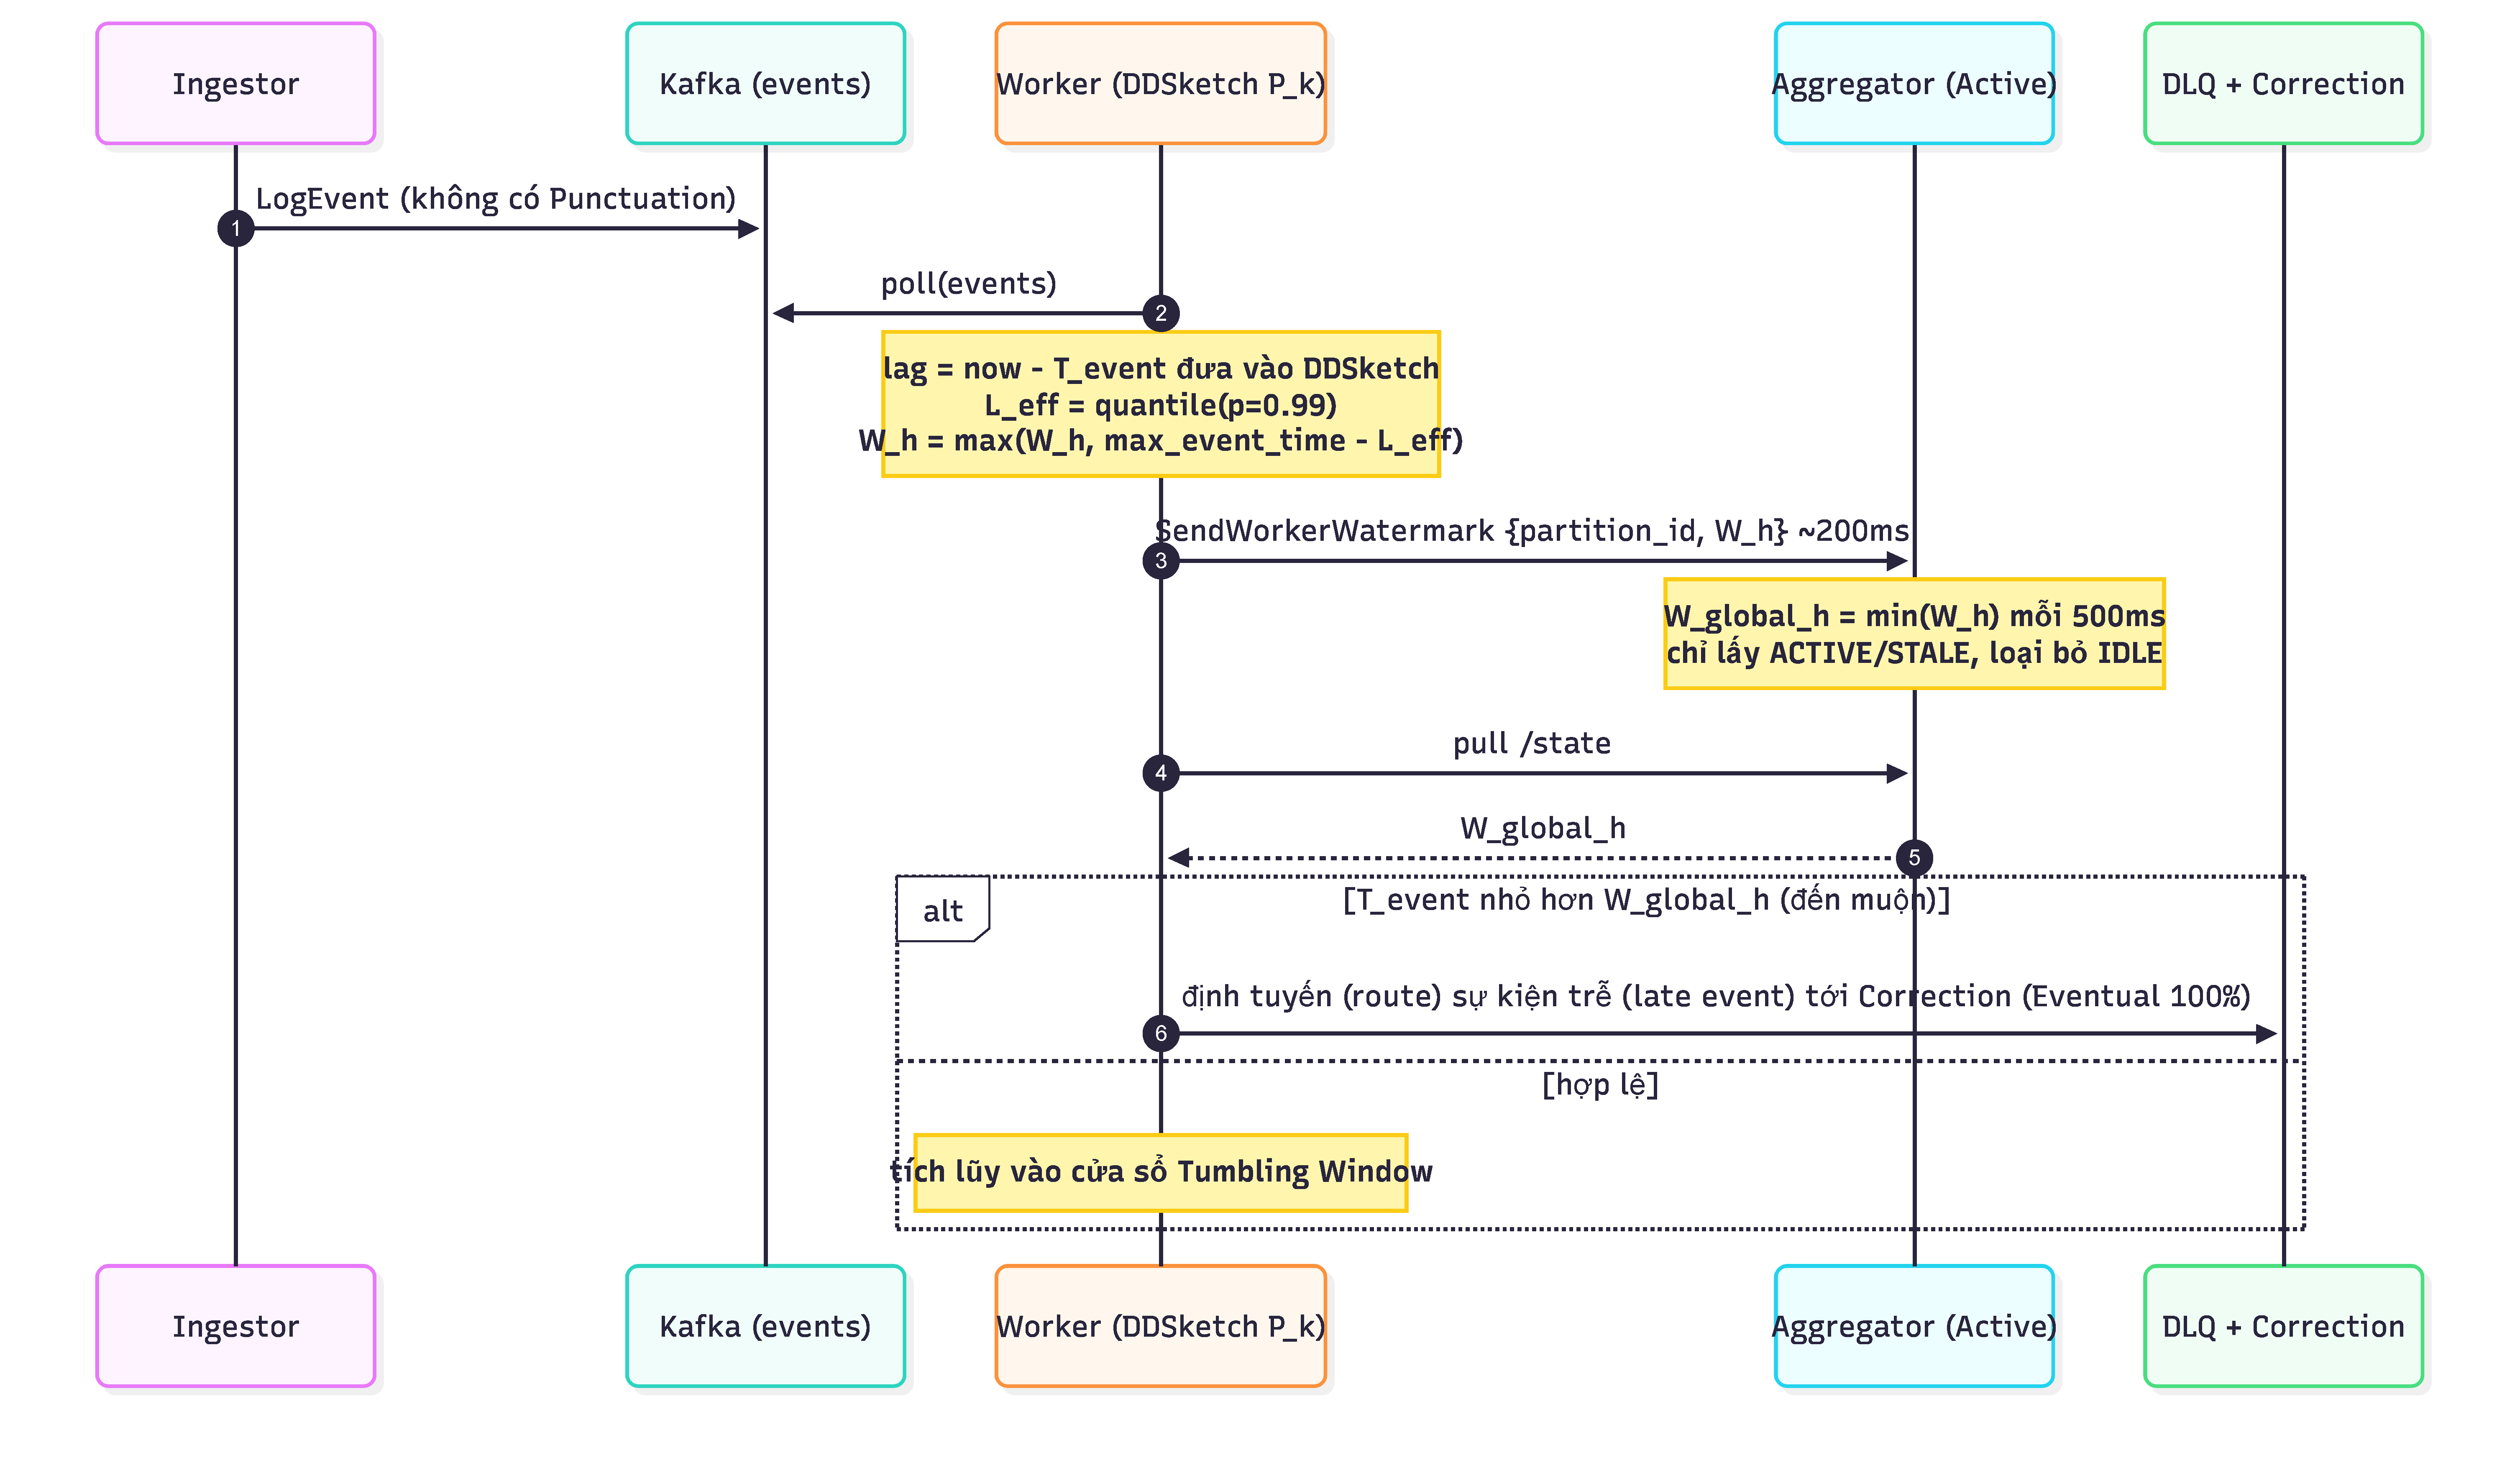
\includegraphics[width=1.15\textwidth]{kafka_bounded_pq.pdf}}
    \caption{Sơ đồ}
    \label{fig:kafka_bounded_pq}
\end{figure}
\textbf{Liên hệ.} Event sau khi qua Bounded PQ mới vào engine từng partition (\ref{sec:node-partition}) để tính watermark (\ref{sec:strict-watermark}/\ref{sec:heuristic-watermark}). Offset Kafka được checkpoint xuống Tier-2 (\ref{sec:tiered-storage}) và là mốc \texttt{seek(}\tcbhighmath{offset + 1}\texttt{)} khi Failback (\ref{sec:failback-5step}). Kafka cũng chở luồng kết quả/DLQ (\ref{sec:heuristic-watermark}) và ingestor-heartbeat (\ref{sec:layer-communication}).

\subsection{4.2 Phản biện: Vì sao thiết kế như vậy}
Mục Kafka + Bounded Priority Queue phải trả lời hai câu hỏi riêng: dữ liệu được giữ bền ở đâu, và out-of-order theo event-time được xử lý ở đâu.
\textbf{Phản đề 1: Ingestor đẩy HTTP trực tiếp vào Worker, bỏ Kafka.}

\begin{itemize}
\item \textbf{Vì sao nghe hợp lý:} ít thành phần hạ tầng hơn, đường đi ngắn hơn, dễ nhìn thấy request/response.
\item \textbf{Lý do bác bỏ:} nếu Worker sập trong lúc nhận hoặc xử lý request, dữ liệu đang bay có thể mất. Không có \tcbhighmath{offset} bền thì worker mới không biết replay từ đâu. Hệ thống cũng mất khả năng pause/resume bằng backpressure vì Ingestor phải tự giữ dữ liệu.
\item \textbf{Kết luận phản biện:} Kafka cần thiết vì nó là log bền vững, có partition, \tcbhighmath{offset} và khả năng replay sau sự cố.
\end{itemize}
\textbf{Phản đề 2: Kafka đã có thứ tự partition, không cần sort ở Worker.}

\begin{itemize}
\item \textbf{Vì sao nghe hợp lý:} Kafka bảo đảm thứ tự record trong một partition theo \tcbhighmath{offset}, nên có vẻ đã đủ để xử lý tuần tự.
\item \textbf{Lý do bác bỏ:} thứ tự \tcbhighmath{offset} không đồng nghĩa với thứ tự event-time. Bài toán window tính theo \tcbhighmath{T_{event}}; nếu event có \tcbhighmath{T_{event}} cũ đến sau \tcbhighmath{offset} mới, engine vẫn cần một lớp sắp tương đối theo event-time trước khi cập nhật window.
\item \textbf{Kết luận phản biện:} Kafka giữ durability và replay; BoundedPriorityQueue xử lý out-of-order theo event-time ở phía Worker. Hai thành phần giải hai vấn đề khác nhau.
\end{itemize}
\textbf{Phản đề 3: Dùng min-heap không giới hạn để giữ đúng event-time hơn.}

\begin{itemize}
\item \textbf{Vì sao nghe hợp lý:} giữ càng nhiều event thì càng có cơ hội sắp đúng theo event-time.
\item \textbf{Lý do bác bỏ:} luồng streaming không có điểm kết thúc tự nhiên; heap không giới hạn sẽ phình RAM và có thể làm Worker chết. Nếu chờ quá lâu để đủ thứ tự tuyệt đối, latency cũng tăng vô hạn.
\item \textbf{Kết luận phản biện:} heap phải bounded bằng \texttt{maxsize} và \tcbhighmath{max\_wait\_ms} để cân bằng giữa sắp event-time, giới hạn bộ nhớ và tiến độ xử lý.
\end{itemize}

\section{5. Thiết kế Tiered Storage}
\label{sec:tiered-storage}

\subsection{5.1 Trình bày chi tiết thiết kế}
\textbf{Ý chính.} Tiered Storage chia state theo vòng đời và yêu cầu truy cập. Tier-1 là RocksDB cục bộ để phục vụ hot path cập nhật từng event. Tier-2 là Shared Volume hoặc checkpoint directory để phục hồi nhanh khi worker crash hoặc partition chuyển chủ. Tier-3 là MinIO/Object Storage để lưu closed window, archive và disaster recovery. Ba tầng vận hành theo ba nhịp độc lập: xử lý nóng, checkpoint định kỳ và archive dài hạn.
\textbf{Bản đồ thiết kế.}
\textbf{Thành phần và trách nhiệm.}

\begin{itemize}
\item \textbf{Tier-1 RocksDB local:} giữ hot state đang được cập nhật theo từng event.
\item \textbf{Tier-2 checkpoint directory/Shared Volume:} giữ checkpoint định kỳ để worker khác phục hồi nhanh.
\item \textbf{Tier-3 MinIO bucket:} giữ closed window, archive và backup phục vụ DR.
\item \textbf{EvictionManager:} điều khiển vòng đời closed window từ local sang object storage rồi purge.
\item \textbf{TieredStorageManager:} gom logic ghi/đọc giữa ba tier và cung cấp API phục hồi state.
\end{itemize}
\textbf{Quan hệ giữa node, partition và tier.}

\begin{itemize}
\item \textbf{Worker node:} là máy/process đang chạy xử lý tại một thời điểm. Một node có thể giữ nhiều partition, ví dụ \texttt{W1} giữ \texttt{P0}, \texttt{P1}, \texttt{P2}.
\item \textbf{Partition:} là đơn vị sở hữu state. Mọi state quan trọng phải gắn với \tcbhighmath{partition\_id}, không gắn cố định với \tcbhighmath{worker\_id}.
\item \textbf{Tier-1:} nằm local trên node đang là owner của partition. Nếu \texttt{P1} đang chạy trên \texttt{W1}, hot state của \texttt{P1} nằm trong RocksDB local của \texttt{W1}.
\item \textbf{Tier-2:} nằm ngoài node hiện tại hoặc ở shared checkpoint path. Checkpoint của \texttt{P1} được định danh theo \tcbhighmath{partition\_id}, nên node khác vẫn đọc được khi \texttt{P1} chuyển owner.
\item \textbf{Tier-3:} nằm trên object storage dùng chung. Closed window/archive của \texttt{P1} cũng dùng key theo partition/window, không phụ thuộc node nào đã tạo ra nó.
\end{itemize}
\textbf{Bảng quan hệ ownership và lưu trữ.}

\begin{table}[H]
\centering
\begin{tabular}{p{2.5cm}p{3.2cm}p{3.2cm}p{6.1cm}}
\toprule
\textbf{Đối tượng} & \textbf{Gắn với node?} & \textbf{Gắn với partition?} & \textbf{Vai trò trong Tiered Storage} \\
\midrule
Worker node & Có, nhưng chỉ tạm thời & Không phải định danh state chính & Chạy engine và giữ Tier-1 local cho các partition đang sở hữu \\
Partition & Có thể đổi node & Có, là định danh chính & Quyết định namespace state, checkpoint, \tcbhighmath{offset} và object key \\
Tier-1 RocksDB local & Có, nằm trên node owner hiện tại & Có, tách theo partition & Hot state nhanh, mất node thì phải phục hồi từ Tier-2 \\
Tier-2 checkpoint & Không phụ thuộc một node cụ thể & Có, key theo partition/checkpoint version & Nơi node mới đọc để nhận partition sau failover/failback \\
Tier-3 MinIO/Object Storage & Không phụ thuộc node & Có, key theo partition/window id & Lưu closed window, archive và backup DR dài hạn \\
\bottomrule
\end{tabular}
\end{table}
\textbf{Luồng lưu trữ: Tier-1 nhận event, Tier-2 checkpoint Tier-1 vào Shared Volume.}
Cách hình dung đơn giản nhất: event của mỗi partition được ghi \textit{ngay} vào Tier-1 — RocksDB cục bộ nằm trên node đang sở hữu partition đó. Định kỳ 10 giây, Tier-2 \textbf{chụp lại nội dung Tier-1} của từng partition (kèm Kafka \tcbhighmath{offset} an toàn) và lưu sang Shared Volume dùng chung. Khi node chết, node mới chỉ cần mount checkpoint của partition trên Shared Volume rồi chạy tiếp; checkpoint đặt tên theo \tcbhighmath{partition\_id} nên không phụ thuộc node cũ. Window đã đóng được đẩy tiếp lên Tier-3 để lưu dài hạn.

\begin{figure}[H]
    \centering
    \makebox[\textwidth][c]{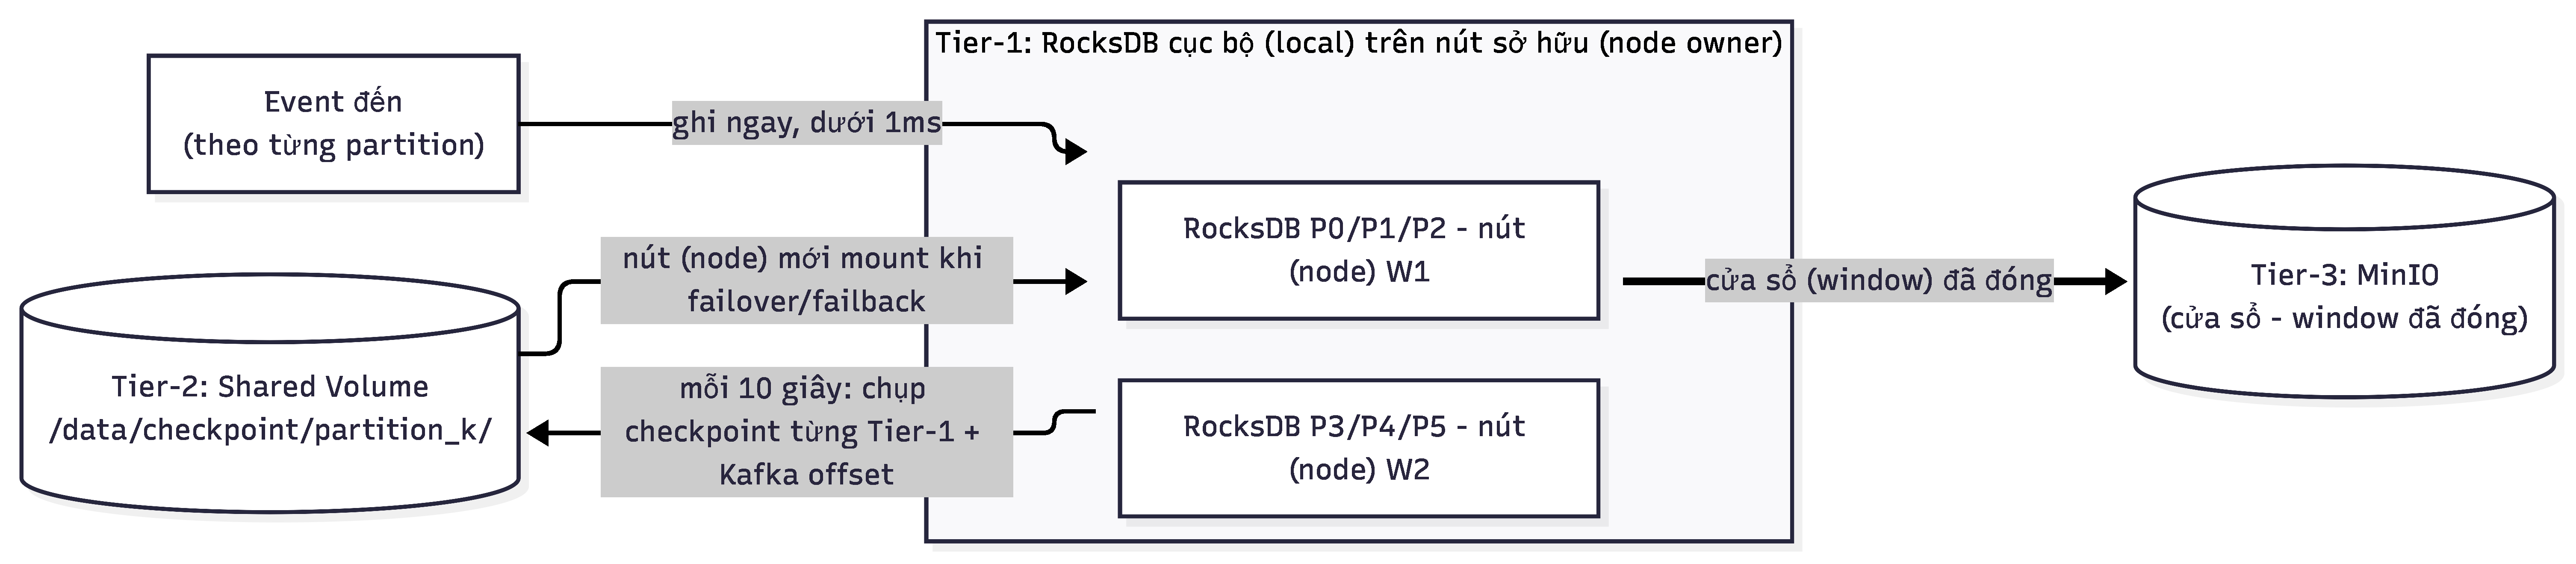
\includegraphics[width=1.15\textwidth]{tiered_storage_flow.pdf}}
    \caption{Sơ đồ luồng (Tier-1 $\rightarrow$ Tier-2 $\rightarrow$ Tier-3)}
    \label{fig:tiered_storage_flow}
\end{figure}
\textbf{Cấu trúc thư mục.} Để dễ hình dung state nằm ở đâu, đây là bố cục thư mục của 3 tầng:

\begin{itemize}
\item \textbf{Tier-1} — cục bộ mỗi node, \texttt{/data/rocksdb/}: mỗi partition một thư mục RocksDB \textbf{riêng} (\texttt{partition\_k/}); bên trong tách namespace bằng tiền tố key: \texttt{ow:} (window đang mở), \texttt{cw:} (window đã đóng), \texttt{si:} (event-id đã thấy, chống trùng), \texttt{meta:} (\tcbhighmath{offset}/watermark).
\item \textbf{Tier-2} — Shared Volume, \texttt{/data/checkpoint/}: mỗi partition một thư mục checkpoint chứa \texttt{metadata.json} (\tcbhighmath{offset}, danh sách window, \tcbhighmath{term}), \texttt{state.db/} (các file SST của RocksDB) và \texttt{\tcbhighmath{sketch}.bin} (state DDSketch — chỉ Heuristic).
\item \textbf{Tier-3} — MinIO: object key theo partition/window cho window đã đóng (\texttt{historical/}), backup DR (\texttt{active\_state\_backup/}) và \texttt{disaster\_recovery/}.
\end{itemize}

\begin{figure}[H]
    \centering
    \makebox[\textwidth][c]{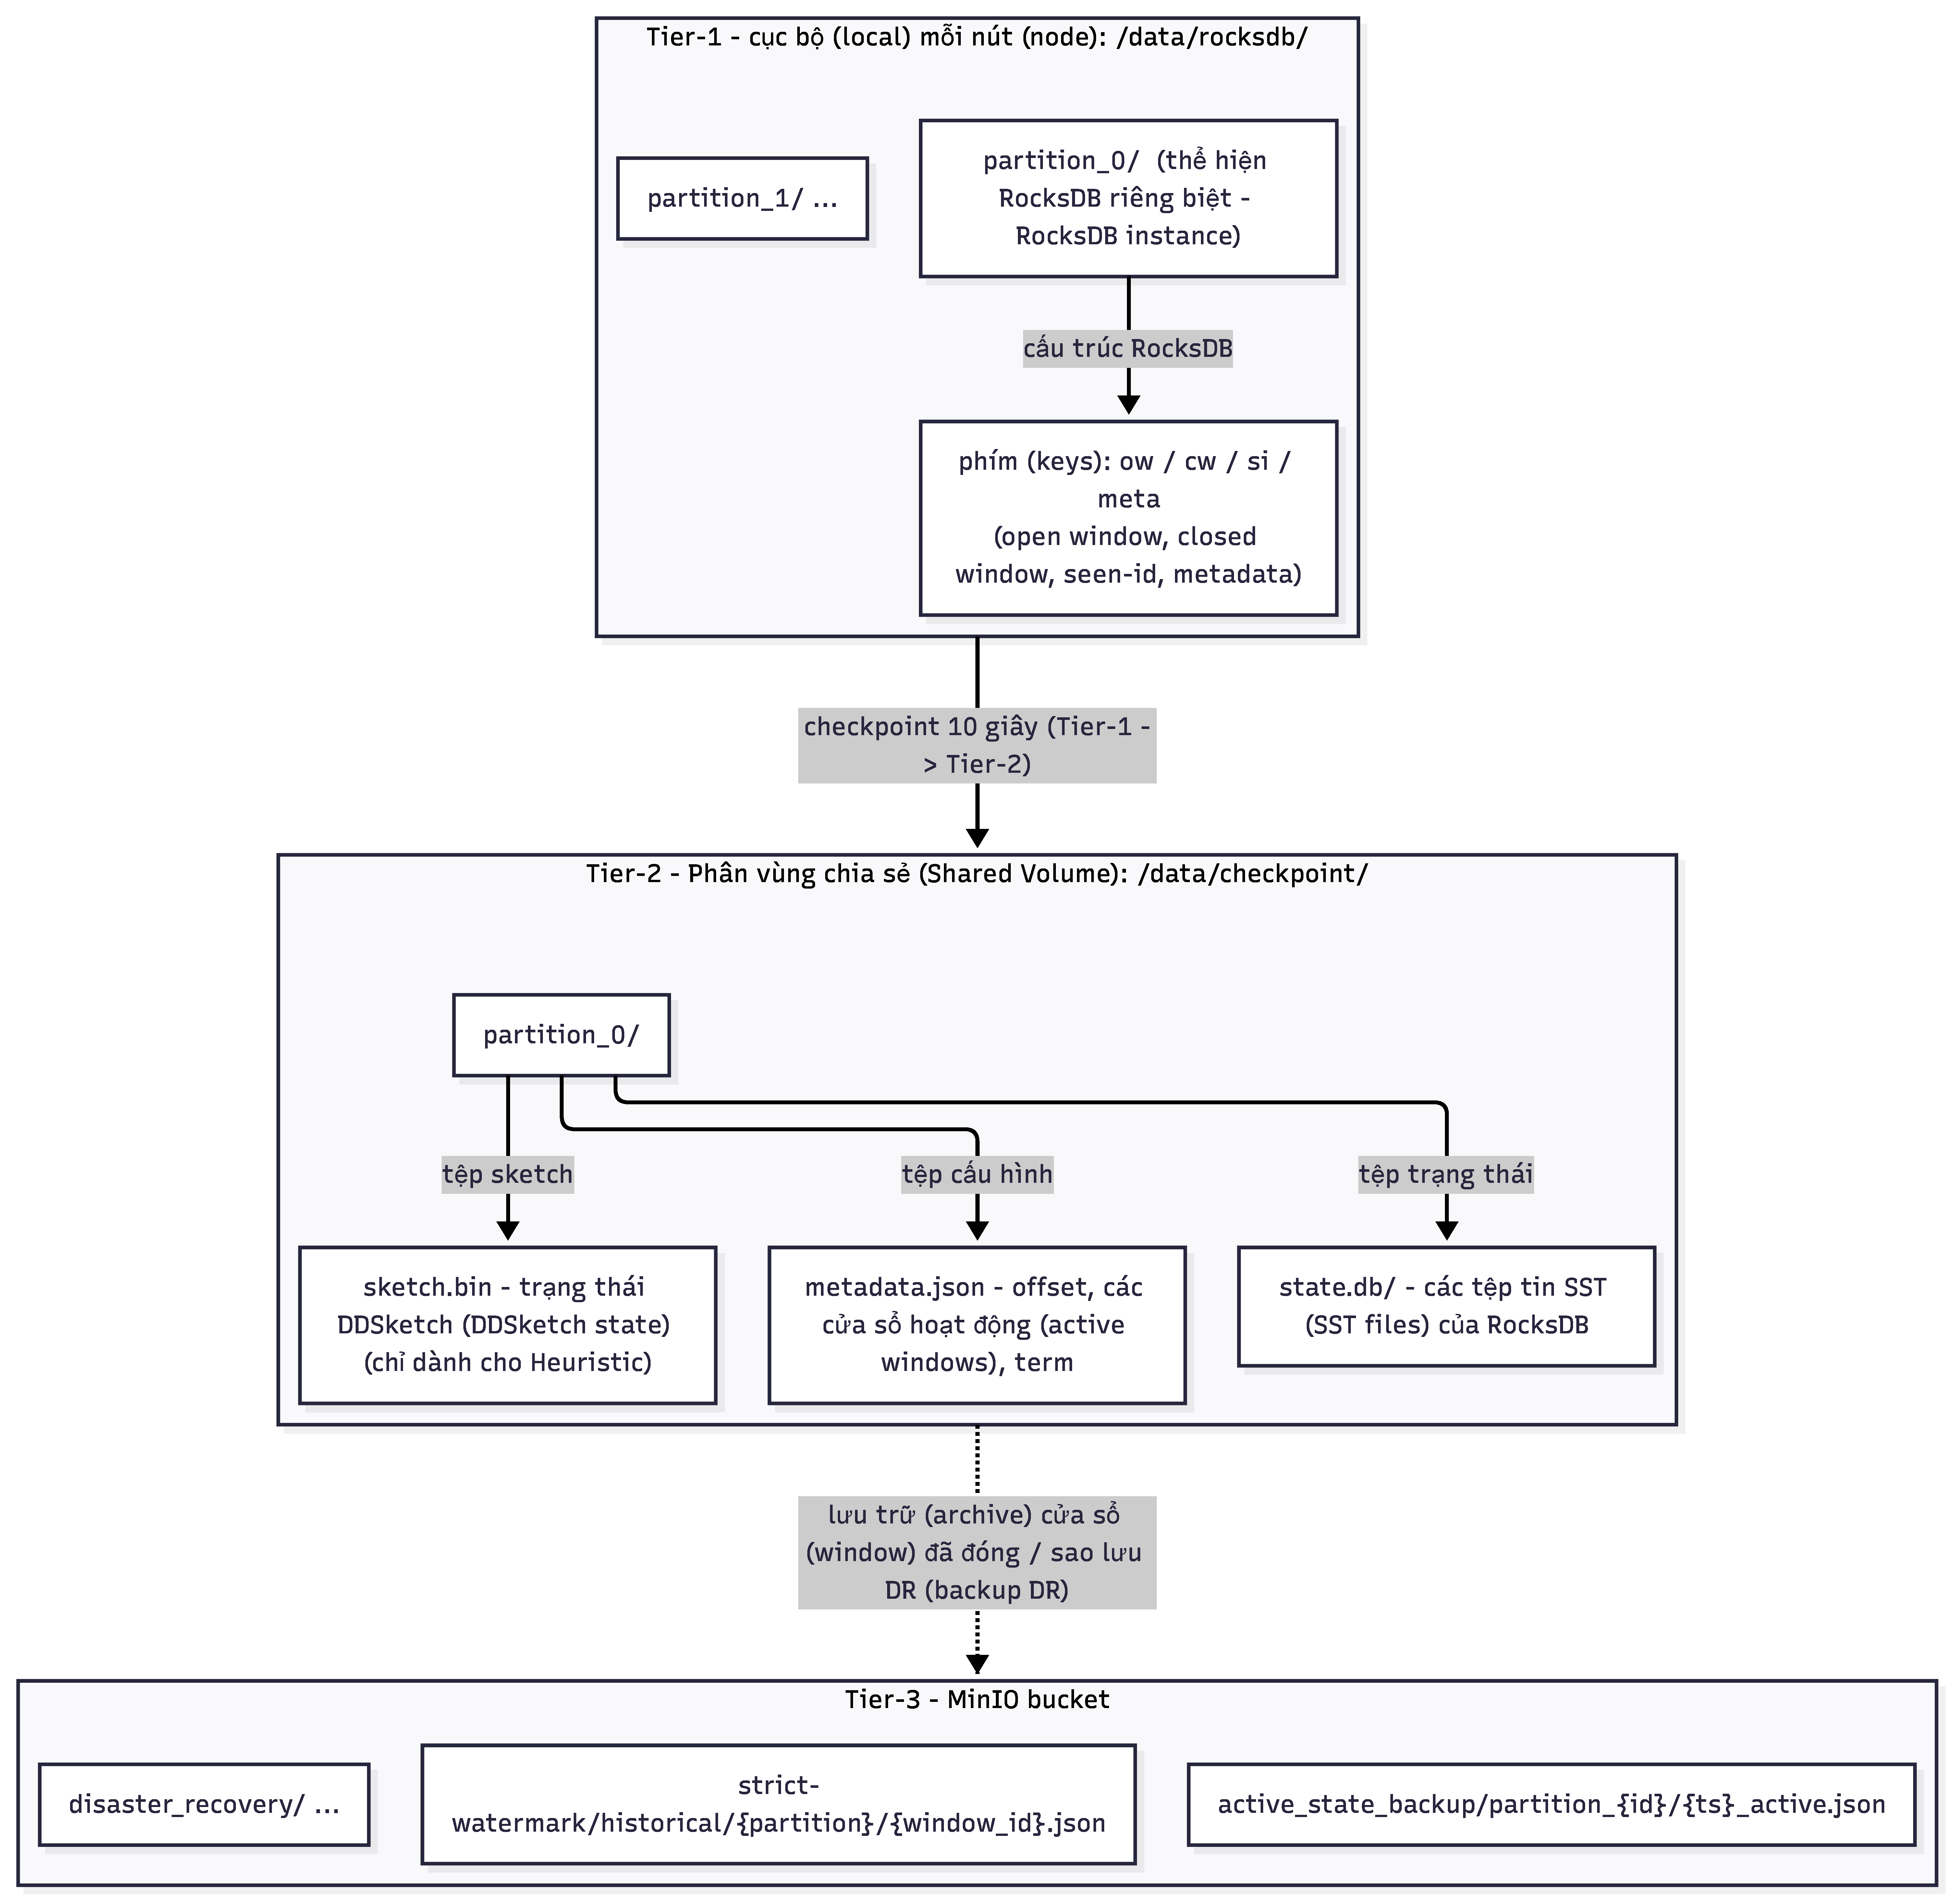
\includegraphics[width=1.15\textwidth]{tiered_storage_layout.pdf}}
    \caption{Sơ đồ cấu trúc thư mục}
    \label{fig:tiered_storage_layout}
\end{figure}
\textbf{Khi partition chuyển node.}

\begin{enumerate}
\item Coordinator quyết định \texttt{P1} chuyển từ \texttt{W1} sang \texttt{W2}.
\item \texttt{W1} dừng xử lý \texttt{P1}, flush Tier-1 của \texttt{P1} ra Tier-2 kèm \tcbhighmath{offset} an toàn.
\item \texttt{W2} tạo hoặc mở RocksDB local mới cho \texttt{P1}.
\item \texttt{W2} đọc checkpoint của \texttt{P1} từ Tier-2, khôi phục open window, dedup state và watermark.
\item \texttt{W2} seek Kafka theo \tcbhighmath{offset} trong checkpoint rồi tiếp tục xử lý \texttt{P1}.
\item Các closed window trước đó của \texttt{P1} vẫn nằm ở Tier-3, vì object key gắn với partition/window chứ không gắn với \texttt{W1}.
\end{enumerate}
\textbf{Dữ liệu ở Tier-1.}

\begin{itemize}
\item \textbf{Open window:} aggregate của window chưa đóng.
\item \textbf{Dedup ids:} id đã xử lý để tránh replay trùng.
\item \textbf{Kafka \tcbhighmath{offset} gần nhất:} \tcbhighmath{offset} đã xử lý/chờ checkpoint.
\item \textbf{Local engine state:} watermark, buffer metadata và trạng thái engine.
\end{itemize}
\textbf{Dữ liệu ở Tier-2.}

\begin{itemize}
\item \textbf{Checkpoint snapshot:} bản chụp state theo chu kỳ.
\item \textbf{SST manifest:} danh sách file/state cần mở lại.
\item \textbf{Offset an toàn:} \tcbhighmath{offset} dùng để \texttt{seek(}\tcbhighmath{offset + 1}\texttt{)} khi worker mới nhận partition.
\item \textbf{Failback state:} trạng thái bàn giao partition nếu đang failback.
\end{itemize}
\textbf{Dữ liệu ở Tier-3.}

\begin{itemize}
\item \textbf{Closed window:} window result đã đóng và cần lưu dài hạn.
\item \textbf{Archive result:} dữ liệu phục vụ audit/đối soát.
\item \textbf{Backup DR:} backup window/state theo chu kỳ dài hơn để giảm RPO.
\item \textbf{Object key:} khóa object theo \texttt{partition/\tcbhighmath{window\_id}} để upload idempotent.
\end{itemize}
\textbf{Luồng ghi.}

\begin{itemize}
\item \textbf{Ghi nóng:} từng event cập nhật Tier-1 ngay.
\item \textbf{Checkpoint:} timer 10s chụp state từ Tier-1 sang Tier-2 kèm \tcbhighmath{offset}.
\item \textbf{Upload closed window:} khi \tcbhighmath{window\_end \le W_{global}}, window đóng được upload lên Tier-3.
\item \textbf{Backup DR:} timer 5 phút backup window đang mở lên Tier-3.
\end{itemize}
\textbf{Luồng đọc/phục hồi.}

\begin{itemize}
\item \textbf{Failover nhanh:} worker mới đọc Tier-2, mở lại state partition và seek Kafka từ \tcbhighmath{offset + 1}.
\item \textbf{Audit/restore xa:} hệ thống đọc object Tier-3 khi cần dữ liệu closed window hoặc DR.
\item \textbf{Retry upload:} nếu upload Tier-3 lỗi, dữ liệu vẫn giữ ở Tier-1/Tier-2 để thử lại.
\end{itemize}
\textbf{Trạng thái vòng đời.}

\begin{itemize}
\item \textbf{\texttt{CLOSED}:} window đã đủ điều kiện đóng.
\item \textbf{\texttt{UPLOADING}:} window đang được upload lên Tier-3.
\item \textbf{\texttt{UPLOADED}:} upload thành công, object đã tồn tại.
\item \textbf{\texttt{PURGED}:} bản local đã được xóa sau khi upload an toàn.
\end{itemize}
\textbf{Giao tiếp.}

\begin{itemize}
\item \textbf{Worker -> RocksDB:} ghi/đọc hot state cục bộ.
\item \textbf{Worker -> Tier-2:} ghi checkpoint định kỳ và đọc checkpoint khi recovery.
\item \textbf{Worker -> MinIO:} upload closed window/backup qua client S3.
\item \textbf{Worker -> Kafka:} sau khi đọc checkpoint, seek về \tcbhighmath{offset} an toàn để replay phần còn thiếu.
\end{itemize}
\textbf{Đầu ra.}

\begin{itemize}
\item \textbf{State nóng:} còn ở Tier-1.
\item \textbf{Checkpoint phục hồi:} nằm ở Tier-2.
\item \textbf{Closed window/archive:} nằm ở Tier-3.
\item \textbf{Recovery point:} cặp state + \tcbhighmath{offset} để worker mới tiếp tục xử lý.
\end{itemize}
\textbf{Bản đồ 3 tier.}

\begin{table}[H]
\centering
\begin{tabular}{p{2.5cm}p{2.2cm}p{2.2cm}p{2.2cm}p{5.5cm}}
\toprule
\textbf{Tier} & \textbf{Khi nào ghi} & \textbf{Dữ liệu chính} & \textbf{Khi nào đọc lại} & \textbf{Vai trò} \\
\midrule
Tier-1 RocksDB local & Ghi liên tục khi từng event được xử lý & Open window, aggregate tạm thời, dedup id, \tcbhighmath{offset} gần nhất, local engine state & Đọc ngay trên hot path khi event tiếp theo cùng window đến & Tốc độ thấp độ trễ, phục vụ cập nhật từng event \\
Tier-2 checkpoint/shared volume & Ghi theo timer 10s hoặc trước khi bàn giao partition & Snapshot state, SST manifest, \tcbhighmath{offset} an toàn, owner/epoch, failback state & Worker mới đọc khi failover/failback để mở lại partition & Phục hồi nhanh khi worker chết hoặc partition đổi owner \\
Tier-3 MinIO/Object Storage & Ghi khi window đã đóng, hoặc backup window đang mở theo timer dài hơn & Closed window, archive result, backup DR, object key theo partition/window & Đọc khi cần audit, restore xa hơn, hoặc Tier-2 không đủ & Lưu dài hạn và disaster recovery \\
\bottomrule
\end{tabular}
\end{table}
\textbf{Cách 3 tier vận hành từng bước.}

\begin{enumerate}
\item Event mới luôn đi vào Tier-1 trước. Engine cập nhật open window trong RocksDB vì thao tác này xảy ra với từng event và cần độ trễ thấp.
\item Sau mỗi chu kỳ checkpoint, Worker chụp state đủ an toàn từ Tier-1 sang Tier-2. Checkpoint phải đi kèm \tcbhighmath{offset} Kafka; nếu chỉ có state mà không có \tcbhighmath{offset} thì recovery sẽ không biết đọc tiếp từ đâu.
\item Khi watermark cho phép đóng window, window chuyển sang trạng thái \texttt{CLOSED}. Worker upload kết quả và metadata lên Tier-3, chuyển trạng thái sang \texttt{UPLOADING}, rồi \texttt{UPLOADED}.
\item Chỉ sau khi upload Tier-3 thành công, Worker mới được purge bản local để giảm dung lượng Tier-1. Nếu upload lỗi, state vẫn giữ ở Tier-1/Tier-2 và retry, tránh mất closed window.
\item Khi worker chết, worker mới đọc Tier-2 để phục hồi nhanh, mở lại RocksDB/state, rồi \texttt{seek(}\tcbhighmath{offset + 1}\texttt{)} trên Kafka để replay phần chưa chắc chắn. Nếu mất cả môi trường cục bộ hoặc cần audit dài hạn, hệ thống dùng Tier-3.
\end{enumerate}
\textbf{Ví dụ vận hành.}

\begin{itemize}
\item \textbf{Vòng đời của cửa sổ \texttt{[10:00:00, 10:00:05)} trên partition \texttt{P1}:}
\item \textbf{Giai đoạn 1 (Ghi nóng vào Tier-1):} Khi các event có event-time trong khoảng \texttt{[10:00:00, 10:00:05)} được xử lý, aggregate tạm thời (ví dụ: sum(sales) = 1500) được ghi trực tiếp vào RocksDB cục bộ của Worker đang chạy \texttt{P1} (Tầng Tier-1). Thao tác đọc/ghi cực nhanh (< 1ms).
\item \textbf{Giai đoạn 2 (Checkpoint sang Tier-2):} Đúng chu kỳ 10 giây, Worker thực hiện flush state của \texttt{P1} từ Tier-1 ghi thành file SST và lưu vào Shared Volume \texttt{/data/checkpoint/partition\_1/} (Tầng Tier-2) kèm theo mốc \tcbhighmath{offset} Kafka an toàn đã xử lý là 500.
\item \textbf{Giai đoạn 3 (Đóng và đẩy lên Tier-3):} Khi watermark toàn cục vượt qua \texttt{10:00:05}, cửa sổ này được đóng. Kết quả chính thức được Worker đẩy lên MinIO bucket (Tầng Tier-3) với object key \texttt{historical/P1/10:00:00-10:00:05.json}. Sau khi MinIO xác nhận lưu trữ thành công, bản ghi cục bộ của cửa sổ này trong RocksDB được giải phóng (evicted/purged) để tiết kiệm ổ đĩa cục bộ.
\item \textbf{Trường hợp sập nguồn:} Nếu Worker bị crash đột ngột ở Offset 505, Worker gánh hộ mới được Coordinator chỉ định. Worker mới chỉ cần đọc checkpoint từ \texttt{/data/checkpoint/partition\_1/} (Tier-2) để khôi phục nhanh state tại Offset 500, sau đó seek consumer Kafka về \tcbhighmath{offset} 501 và replay 5 event tiếp theo để xử lý tiếp mà không phải quét lại từ đầu luồng Kafka.
\end{itemize}

\begin{figure}[H]
    \centering
    \makebox[\textwidth][c]{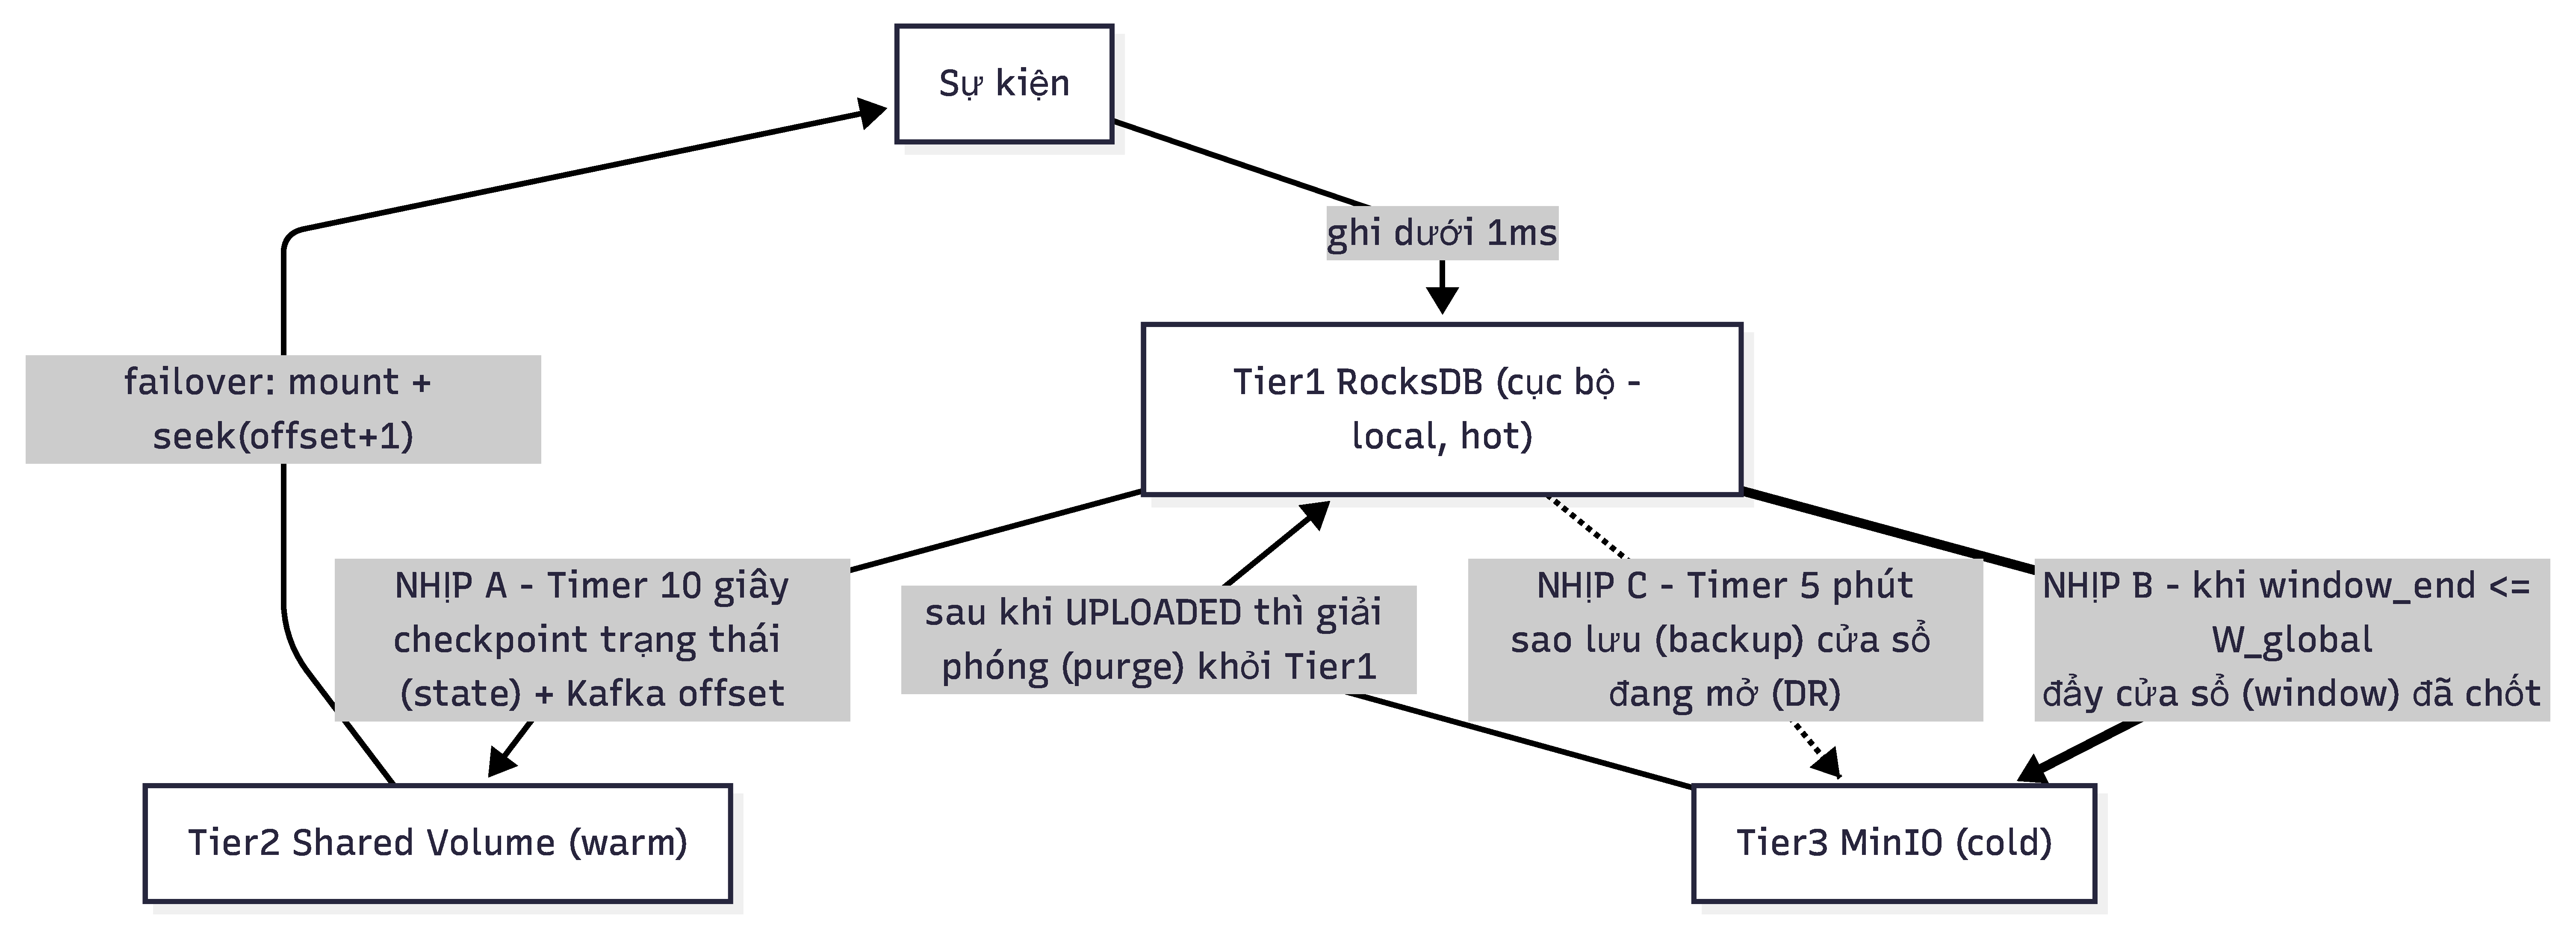
\includegraphics[width=1.15\textwidth]{tiered_storage_cycles.pdf}}
    \caption{Sơ đồ luồng 3 tầng}
    \label{fig:tiered_storage_cycles}
\end{figure}

\begin{figure}[H]
    \centering
    \makebox[\textwidth][c]{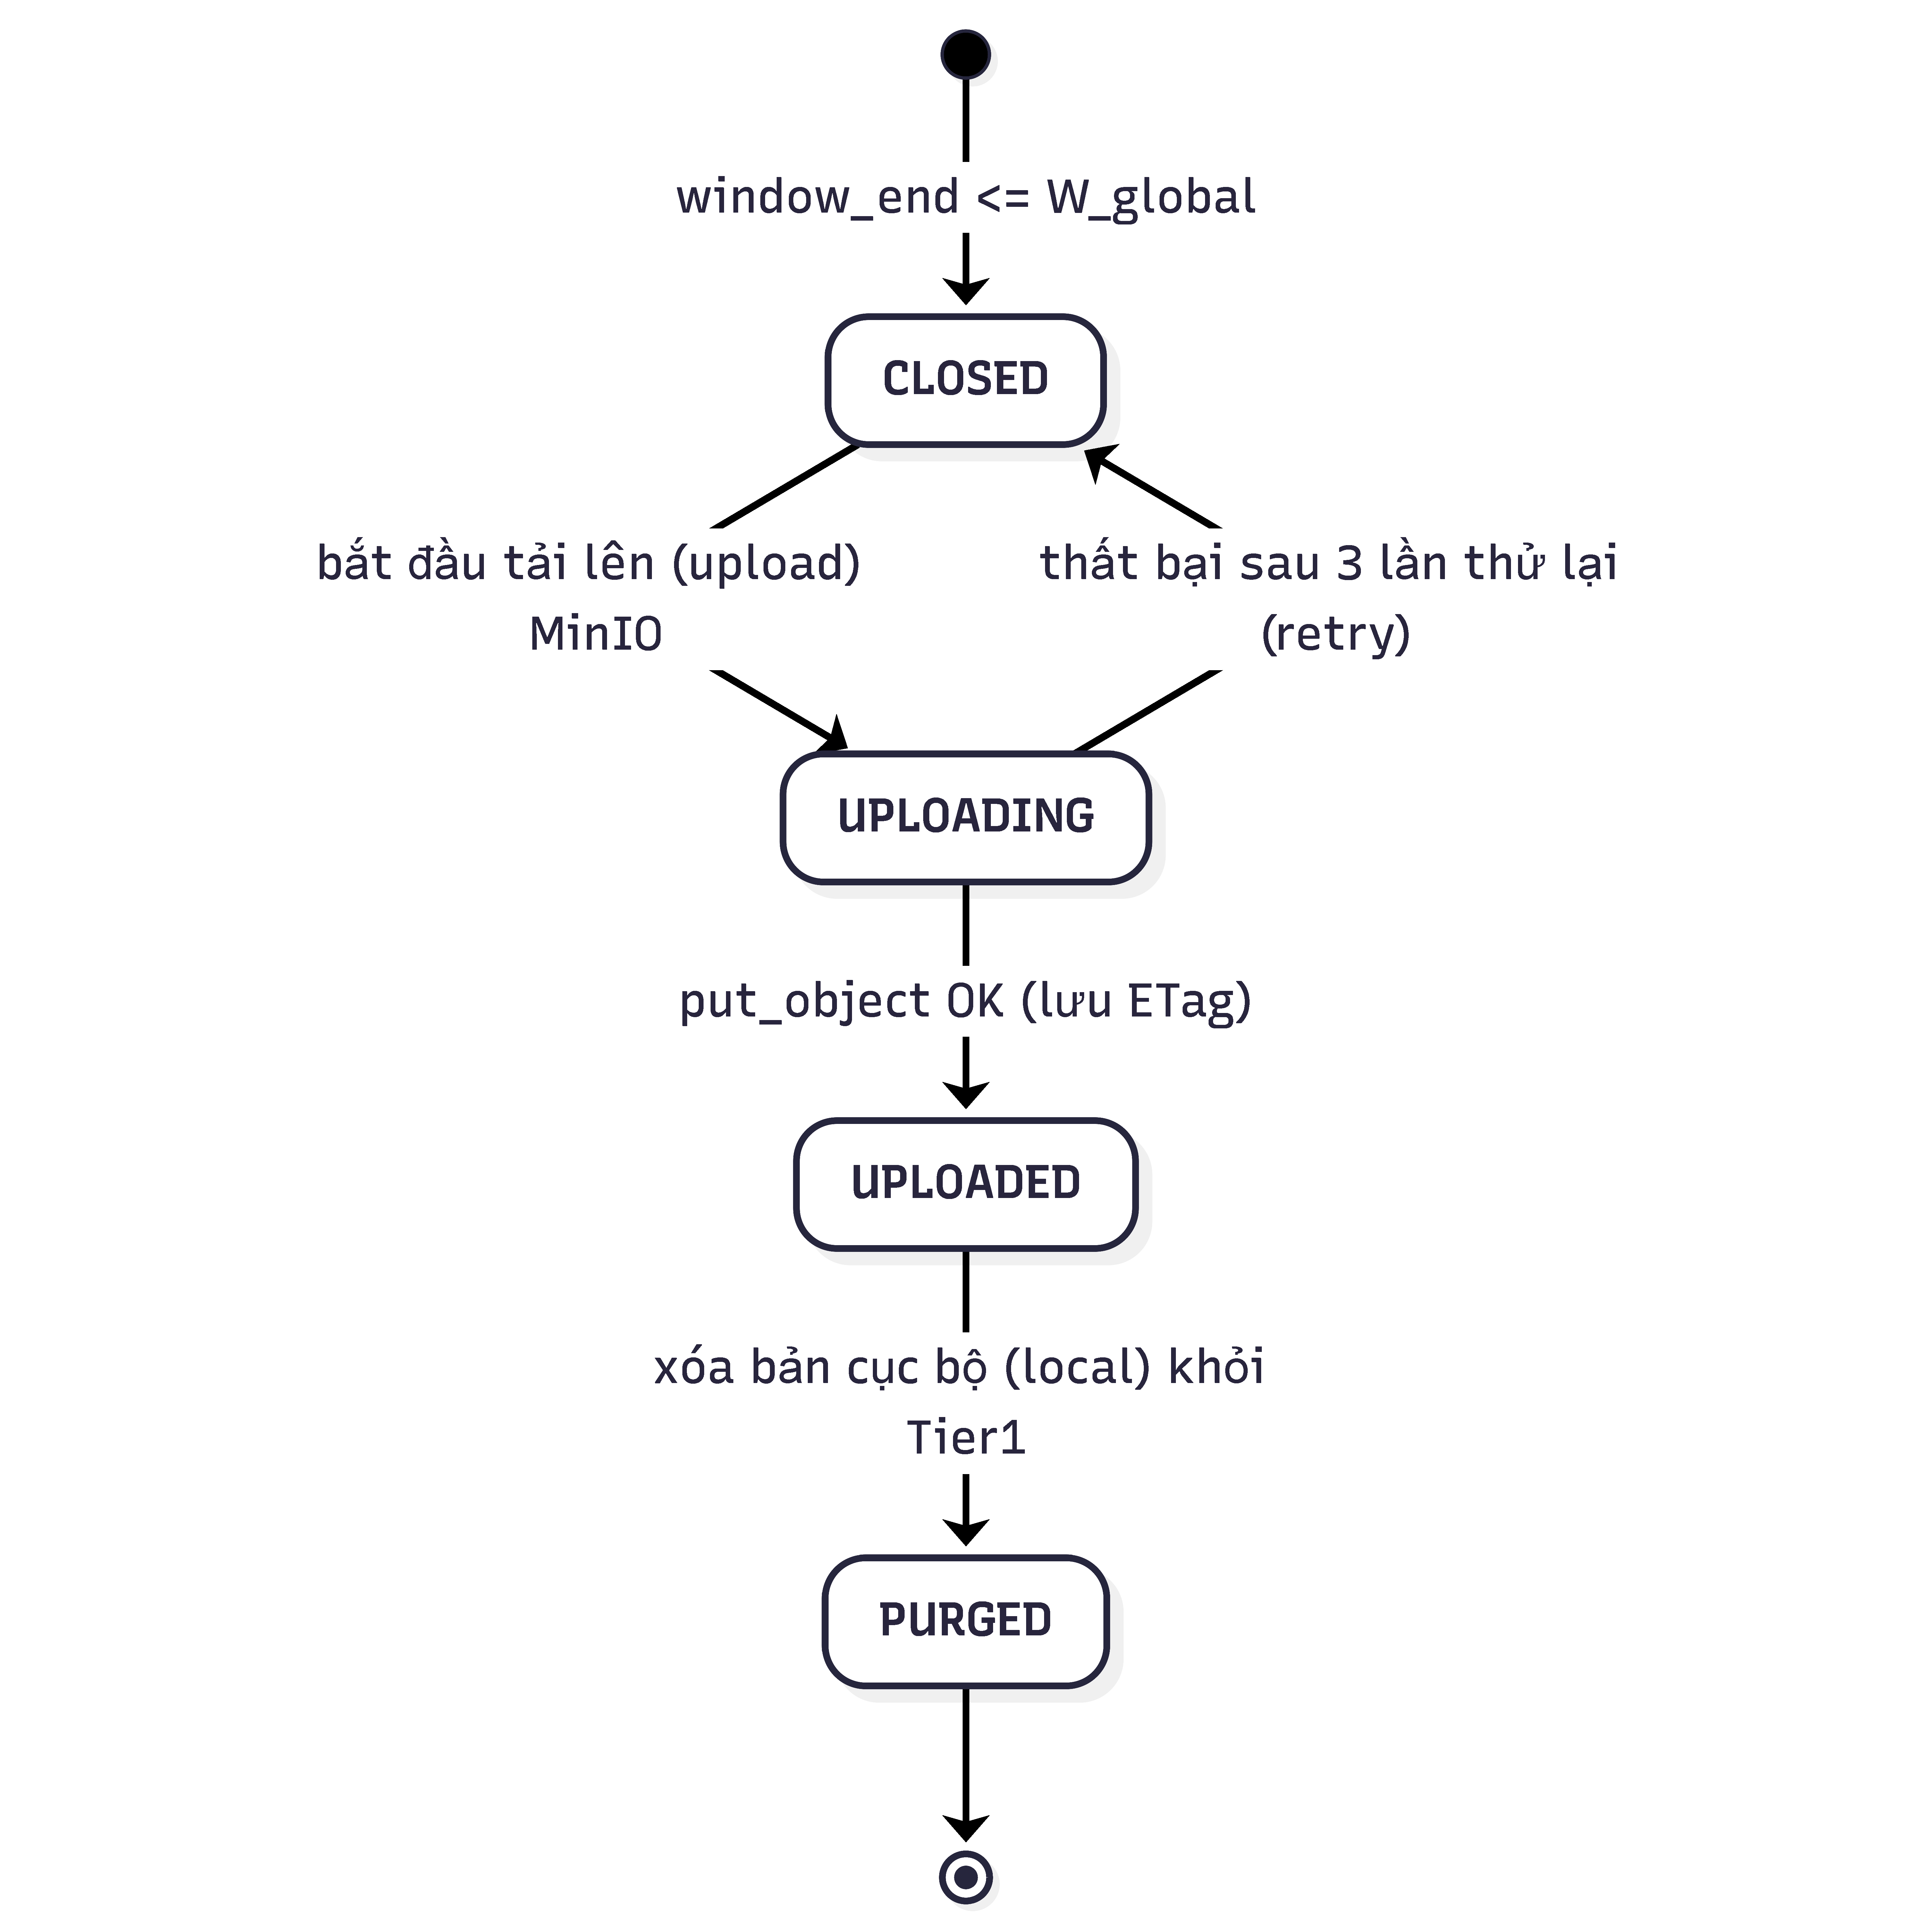
\includegraphics[width=1.15\textwidth]{eviction_state_machine.pdf}}
    \caption{Sơ đồ vòng đời window đã chốt}
    \label{fig:eviction_state_machine}
\end{figure}
\textbf{Liên hệ.} State ở 3 tầng đến từ engine mỗi partition (\ref{sec:node-partition}); checkpoint Tier-2 chính là thứ Failback (\ref{sec:failback-5step}) đọc lại để node mới tiếp quản; \tcbhighmath{offset} đi kèm checkpoint là mốc replay Kafka (\ref{sec:kafka-pq}). Đường ghi/đọc storage là một trong các kênh ở \ref{sec:layer-communication}.

\subsection{5.2 Phản biện: Vì sao thiết kế như vậy}
Mục Tiered Storage phải phản biện rõ vì sao không thể dùng một tầng lưu trữ duy nhất. Ba yêu cầu của state là khác nhau: hot path phải nhanh, failover phải phục hồi được, archive/DR phải bền dài hạn.
\textbf{Phản đề 1: Chỉ dùng Tier-1 RocksDB local.}

\begin{itemize}
\item \textbf{Vì sao nghe hợp lý:} RocksDB rất nhanh, có WAL, phù hợp cập nhật từng event và đơn giản hơn so với ba tầng.
\item \textbf{Lý do bác bỏ:} RocksDB local gắn với node đang chạy. Khi node chết, node khác không thể chắc chắn mở cùng state ngay lập tức; thư mục RocksDB còn có lock độc quyền và có thể nằm trên disk cục bộ đã mất. Nếu chỉ có Tier-1, failover không có checkpoint bền để worker mới đọc lại.
\item \textbf{Kết luận phản biện:} Tier-1 chỉ phù hợp hot path, không đủ để bảo vệ recovery khi worker hoặc máy chứa state chết.
\end{itemize}
\textbf{Phản đề 2: Dùng Tier-1 + Tier-2 là đủ, không cần Tier-3.}

\begin{itemize}
\item \textbf{Vì sao nghe hợp lý:} Tier-2 đã có checkpoint để failover, nên nhìn qua có vẻ đã giải quyết được sự cố worker chết.
\item \textbf{Lý do bác bỏ:} Tier-2 thường là shared volume/checkpoint gần hệ thống runtime; nó phục vụ phục hồi nhanh, không phải lưu trữ dài hạn hoặc DR. Nếu shared volume lỗi, checkpoint của nhiều partition có thể mất cùng lúc. Nó cũng không phải nơi tốt để giữ closed window/archive lâu dài.
\item \textbf{Kết luận phản biện:} Tier-2 giải bài toán failover nhanh, nhưng chưa giải bài toán lưu lâu dài, audit và disaster recovery.
\end{itemize}
\textbf{Phản đề 3: Chỉ dùng Tier-3 MinIO/Object Storage cho mọi state.}

\begin{itemize}
\item \textbf{Vì sao nghe hợp lý:} MinIO/S3 bền, dùng chung giữa node, không phụ thuộc disk cục bộ.
\item \textbf{Lý do bác bỏ:} object storage có latency cao hơn nhiều so với RocksDB local và không phù hợp cập nhật nhỏ theo từng event. Nếu mọi open window đều đọc/ghi qua MinIO, hot path sẽ chậm, tốn băng thông và khó đạt latency xử lý streaming.
\item \textbf{Kết luận phản biện:} Tier-3 phù hợp archive/DR, không phù hợp làm state store nóng cho từng event.
\end{itemize}
\textbf{Kết luận chung:} ba tier không phải thêm cho phức tạp, mà vì mỗi tier bảo vệ một thuộc tính riêng: Tier-1 bảo vệ tốc độ, Tier-2 bảo vệ failover, Tier-3 bảo vệ lưu dài hạn và DR.

\section{6. Thiết kế Coordinator \& Aggregator}
\label{sec:coordinator-aggregator}

\subsection{6.1 Trình bày chi tiết thiết kế}
\textbf{Ý chính.} Hệ thống tách Coordinator và Aggregator vì Strict và Heuristic có mức cam kết khác nhau. Coordinator phục vụ Strict, chạy theo mô hình HA/Raft, có Leader tính \tcbhighmath{W_{global}}, quản lý ownership partition, failover/failback và fencing. Aggregator phục vụ Heuristic, dùng active-standby nhẹ hơn, chỉ gom \tcbhighmath{W_h} thành \tcbhighmath{W_{global\_h}} và cung cấp trạng thái khả dụng.
\textbf{Bản đồ thiết kế.}
\textbf{Coordinator Strict.}

\begin{itemize}
\item \textbf{Nhận heartbeat:} đọc trạng thái worker, partition id, local watermark và \tcbhighmath{offset}/status.
\item \textbf{Lưu partition status:} biết partition nào active, stale, idle, failed hoặc đang reassign.
\item \textbf{Tính \tcbhighmath{W_{global}}:} lấy min watermark trên partition hợp lệ và giữ watermark đơn điệu.
\item \textbf{Kiểm tra fencing token:} từ chối lệnh cũ khi leader/\tcbhighmath{term} đã thay đổi.
\item \textbf{Phát hiện worker lỗi:} dùng heartbeat timeout để đánh dấu worker failed.
\item \textbf{Ra lệnh reassign/failback:} chuyển quyền sở hữu partition qua quy trình có \tcbhighmath{term} và command id.
\end{itemize}
\textbf{Aggregator Heuristic.}

\begin{itemize}
\item \textbf{Nhận \tcbhighmath{W_h}:} lấy watermark heuristic từ Worker theo partition.
\item \textbf{Lưu trạng thái partition:} biết partition active/idle để tính min đúng với Heuristic.
\item \textbf{Tính \tcbhighmath{W_{global\_h}}:} lấy min trên partition active.
\item \textbf{Duy trì active/standby:} Active phục vụ request, Standby giám sát để tiếp quản.
\item \textbf{Không điều phối ownership:} Aggregator không phát lệnh chuyển partition.
\end{itemize}
\textbf{Dữ liệu điều khiển vào.}

\begin{itemize}
\item \textbf{Heartbeat:} worker id, partition id, local watermark, \tcbhighmath{offset}/status.
\item \textbf{Watermark heuristic:} \tcbhighmath{W_h} của từng partition.
\item \textbf{Raft/lock signal:} \tcbhighmath{term}, vote/state hoặc active/standby heartbeat.
\end{itemize}
\textbf{Dữ liệu điều khiển ra.}

\begin{itemize}
\item \textbf{\tcbhighmath{W_{global}}:} watermark toàn cục cho Strict.
\item \textbf{\tcbhighmath{W_{global\_h}}:} watermark toàn cục cho Heuristic.
\item \textbf{Command điều phối:} reassign, pause, flush, resume trong Strict.
\item \textbf{Fencing metadata:} \tcbhighmath{term} và command id đi kèm lệnh.
\end{itemize}
\textbf{Trạng thái cần giữ.}

\begin{itemize}
\item \textbf{Partition owner/status:} ai đang sở hữu partition và trạng thái hiện tại.
\item \textbf{Global watermark:} \tcbhighmath{W_{global}} hoặc \tcbhighmath{W_{global\_h}}.
\item \textbf{Raft \tcbhighmath{term}:} \tcbhighmath{term} hiện tại của Coordinator Strict.
\item \textbf{Failback state:} bước failback đang chạy nếu có.
\item \textbf{Aggregator lock state:} Active nào đang giữ quyền phục vụ.
\end{itemize}
\textbf{Giao tiếp.}

\begin{itemize}
\item \textbf{Worker -> Coordinator:} heartbeat Strict mỗi 1s.
\item \textbf{Worker -> Coordinator:} pull state/watermark khoảng 500ms.
\item \textbf{Coordinator Leader -> Follower:} replicate state và commit khi đạt đa số.
\item \textbf{Worker -> Aggregator:} gửi \tcbhighmath{W_h} chu kỳ ngắn.
\item \textbf{Standby -> Active/lock service:} giám sát heartbeat để takeover khi Active lỗi.
\end{itemize}
\textbf{Đầu ra.}

\begin{itemize}
\item \textbf{Cho Worker Strict:} \tcbhighmath{W_{global}} và lệnh điều phối partition.
\item \textbf{Cho Worker Heuristic:} \tcbhighmath{W_{global\_h}}.
\item \textbf{Cho vận hành:} trạng thái owner/active/standby để quan sát control plane.
\end{itemize}
\textbf{Cách chạy từng bước.}

\begin{enumerate}
\item Trong Strict, Worker gửi heartbeat theo partition cho Coordinator Leader. Heartbeat chứa worker id, partition id, local watermark, \tcbhighmath{offset}/status và \tcbhighmath{term}/epoch liên quan đến quyền sở hữu.
\item Leader cập nhật bảng partition ownership, bảng watermark và trạng thái worker. Nếu phát hiện worker quá hạn heartbeat, Leader đánh dấu worker lỗi và tạo lệnh reassign partition.
\item Trước khi lệnh điều phối có hiệu lực, Leader replicate thay đổi sang Follower. Khi đạt đa số, lệnh mới được coi là committed. Term/fencing giúp Worker từ chối lệnh cũ phát ra từ Leader đã hết quyền.
\item \tcbhighmath{W_{global}} trong Strict được tính từ local watermark của partition, nhưng quyết định ownership/failback cũng nằm ở Coordinator. Vì vậy Coordinator không chỉ là "máy lấy min", mà là control plane có quyền điều phối.
\item Trong Heuristic, Aggregator Active nhận \tcbhighmath{W_h}, tính \tcbhighmath{W_{global\_h}} và phục vụ Worker. Standby chỉ giám sát lock/heartbeat. Nếu Active mất, Standby chiếm lock và tiếp tục tổng hợp watermark, không cần replay lệnh ownership phức tạp như Coordinator.
\end{enumerate}
\textbf{Ví dụ vận hành.}

\begin{itemize}
\item \textbf{Kịch bản phân tách mạng (Network Partition) trong cụm Strict:}
\item Coordinator Leader hiện tại đang chạy ở Term 2, giao tiếp với Worker \texttt{W1} đang gánh partition \texttt{P1}.
\item Do sự cố mạng, Coordinator Leader cũ bị cô lập hoàn toàn khỏi cụm nhưng vẫn cố gửi lệnh reassign \texttt{P1} sang \texttt{W2} với Term 2.
\item Trong lúc đó, các Coordinator Follower bầu ra Leader mới với Term 3. Leader mới gán \texttt{P1} sang \texttt{W3} với Term 3.
\item Khi Worker nhận được lệnh từ Leader cũ (Term 2) và Leader mới (Term 3), nhờ có cơ chế \tcbhighmath{term} (Fencing Term), Worker lập tiếp từ chối lệnh mang Term 2 thấp hơn và chỉ chấp nhận lệnh từ Leader mới mang Term 3.
\item \textbf{Kịch bản mất điện trong cụm Heuristic:}
\item Aggregator Active thu thập Heuristic Watermark \tcbhighmath{W_h} từ các Worker bị crash.
\item Aggregator Standby lập tức phát hiện khóa (lease/lock) của Active bị mất, chiếm quyền điều hành và tiếp tục nhận các bản tin gRPC \tcbhighmath{W_h} từ Worker để tổng hợp \tcbhighmath{W_{global\_h}}. Quá trình chuyển đổi chỉ mất < 2 giây. Các event trễ phát sinh trong 2 giây này sẽ đi vào DLQ và được sửa lại bằng Correction sau đó, không cần cơ chế đồng thuận Raft phức tạp.
\end{itemize}

\begin{figure}[H]
    \centering
    \makebox[\textwidth][c]{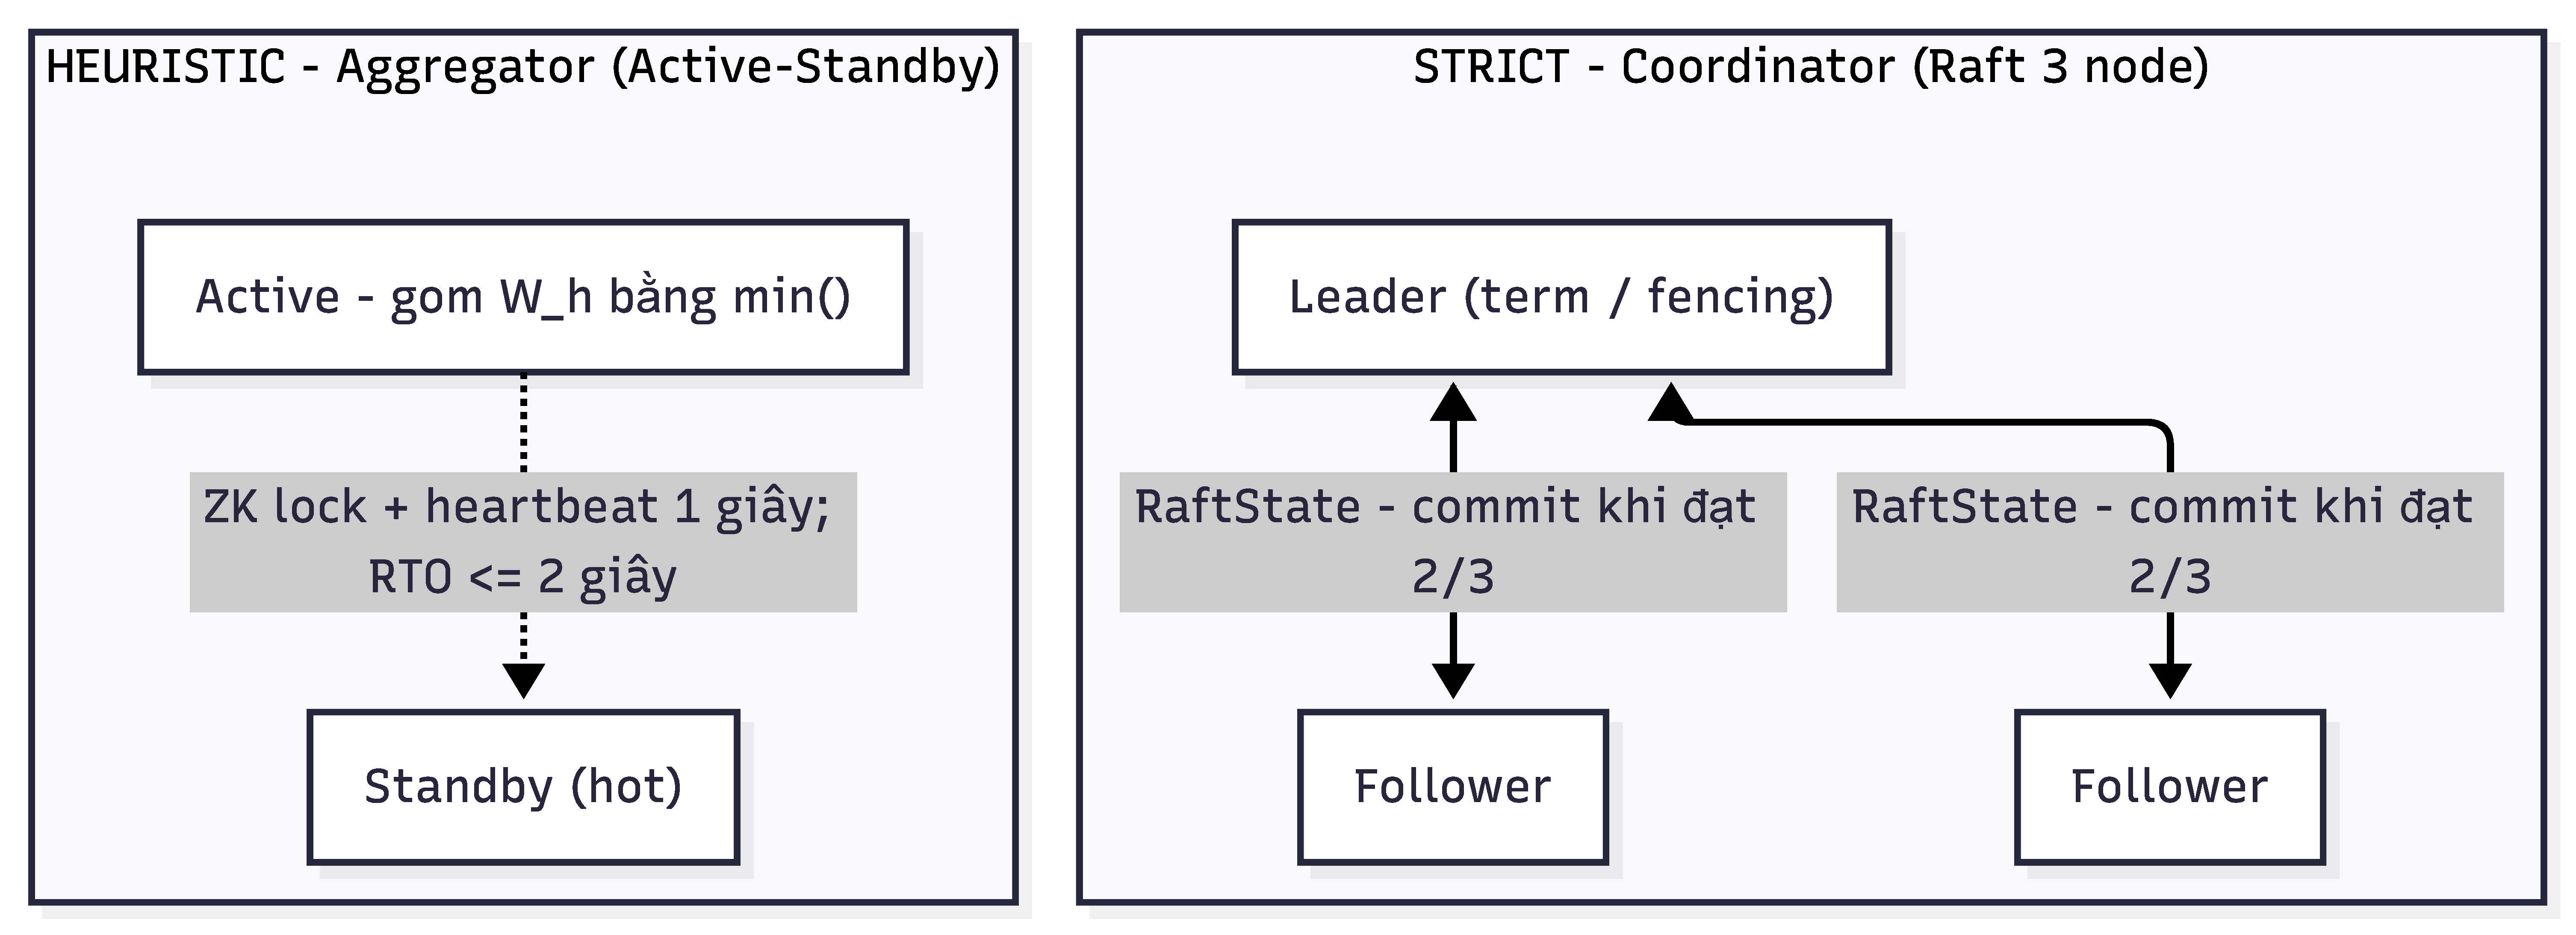
\includegraphics[width=1.15\textwidth]{coordinator_vs_aggregator.pdf}}
    \caption{Sơ đồ}
    \label{fig:coordinator_vs_aggregator}
\end{figure}
\textbf{Liên hệ.} Control plane nhận watermark \textit{map} từ node (\ref{sec:node-partition}) qua kênh control (\ref{sec:layer-communication}), hợp nhất thành \tcbhighmath{W_{global}}/\tcbhighmath{W_{global\_h}} rồi trả lại để engine đóng window (\ref{sec:strict-watermark}/\ref{sec:heuristic-watermark}). Riêng Coordinator còn giữ ownership và điều phối Failback (\ref{sec:failback-5step}); fencing token bảo vệ exactly-once đã cam kết ở \ref{sec:strict-watermark}.

\subsection{6.2 Phản biện: Vì sao thiết kế như vậy}
Mục Coordinator/Aggregator phải giải thích rõ vì sao hai mode không dùng chung một control plane. Strict cần quyền điều phối có fencing; Heuristic chỉ cần tổng hợp watermark nhẹ và chấp nhận correction.
\textbf{Phản đề 1: Strict chỉ cần một khóa active/passive, không cần Raft.}

\begin{itemize}
\item \textbf{Vì sao nghe hợp lý:} hệ thống chỉ cần một Coordinator active tại một thời điểm; khóa ZooKeeper hoặc file lock có vẻ đủ để bầu leader.
\item \textbf{Lý do bác bỏ:} Coordinator Strict không chỉ tính \texttt{min(watermark)}, mà còn ra lệnh chuyển ownership partition. Nếu Leader cũ bị cô lập rồi sống lại, nó có thể phát lệnh cũ song song với Leader mới. Không có \tcbhighmath{term}/fencing, Worker không biết lệnh nào hợp lệ, dẫn tới hai Worker cùng xử lý một partition.
\item \textbf{Kết luận phản biện:} Strict cần Raft/fencing vì lệnh điều phối partition phải có \tcbhighmath{term} tăng đơn điệu và phải được replicate trước khi thực thi.
\end{itemize}
\textbf{Phản đề 2: Heuristic cũng nên dùng Raft cho chắc chắn.}

\begin{itemize}
\item \textbf{Vì sao nghe hợp lý:} đã có cơ chế Raft cho Strict, dùng lại cho Aggregator có vẻ tăng độ an toàn.
\item \textbf{Lý do bác bỏ:} Aggregator không điều phối ownership partition và không cam kết exactly-once tức thời. Nếu Aggregator failover chậm một nhịp, tác động chính là watermark heuristic trễ hoặc late event tăng; các sai lệch này được hấp thụ bằng DLQ/correction. Raft sẽ tăng latency và độ phức tạp nhưng không bảo vệ thêm thuộc tính cốt lõi của Heuristic.
\item \textbf{Kết luận phản biện:} Coordinator Strict cần nhất quán mạnh; Aggregator Heuristic chỉ cần availability nhẹ. Tách hai control plane giúp mỗi mode trả đúng chi phí cho cam kết của nó.
\end{itemize}

\section{7. Giao tiếp giữa các Layer}
\label{sec:layer-communication}

\subsection{7.1 Trình bày chi tiết thiết kế}
\textbf{Ý chính.} Hệ thống không dùng một giao thức cho mọi thứ. Giao tiếp giữa các layer được tách theo bản chất dữ liệu: Kafka cho data plane, gRPC cho control plane, HTTP cho quan sát và thao tác vận hành, còn storage client phục vụ state/checkpoint/archive.
\textbf{Bản đồ thiết kế.}
\textbf{Kafka data plane.}

\begin{itemize}
\item \textbf{Payload:} event, punctuation, result, audit và DLQ.
\item \textbf{Người gửi:} Ingestor hoặc Worker.
\item \textbf{Người nhận:} Worker, result consumer, audit consumer hoặc DLQ/correction pipeline.
\item \textbf{Yêu cầu chính:} bền, partitioned, replay được bằng \tcbhighmath{offset}.
\end{itemize}

\begin{figure}[H]
    \centering
    \makebox[\textwidth][c]{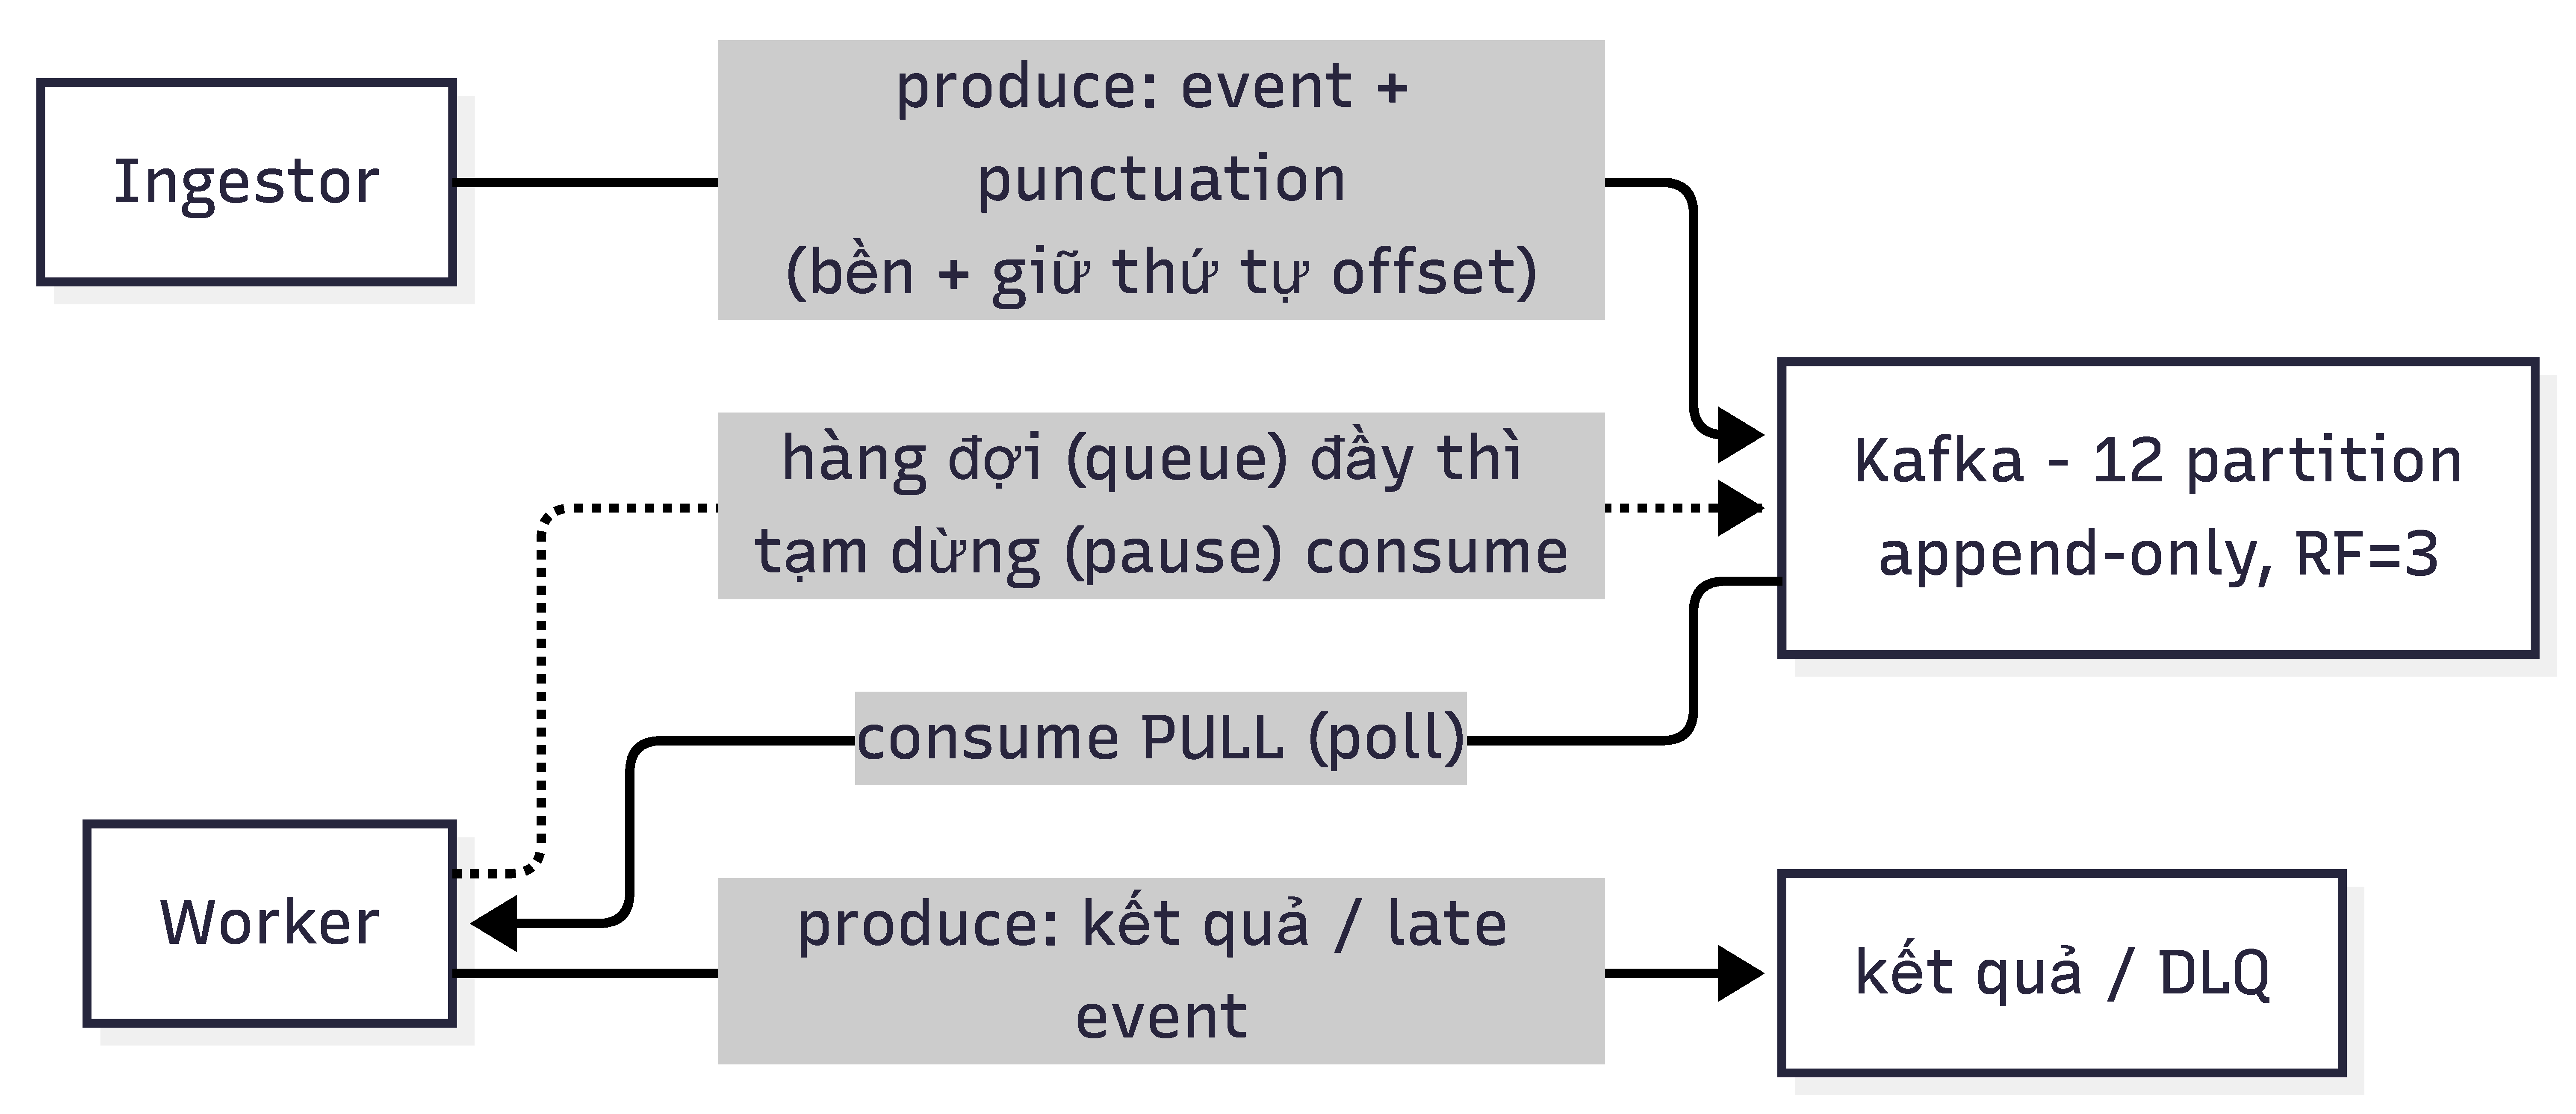
\includegraphics[width=1.15\textwidth]{comm_ingest_data.pdf}}
    \caption{Sơ đồ tầng dữ liệu (Ingestor $\leftrightarrow$ Kafka $\leftrightarrow$ Worker)}
    \label{fig:comm_ingest_data}
\end{figure}
\textbf{gRPC control plane.}

\begin{itemize}
\item \textbf{Payload:} heartbeat, watermark, Raft vote/state, worker watermark, lệnh reassign/failback.
\item \textbf{Người gửi:} Worker, Coordinator, Aggregator hoặc Raft peer.
\item \textbf{Người nhận:} Coordinator, Aggregator, Worker hoặc Raft peer.
\item \textbf{Yêu cầu chính:} schema rõ, latency thấp, phù hợp RPC nội bộ.
\end{itemize}

\begin{figure}[H]
    \centering
    \makebox[\textwidth][c]{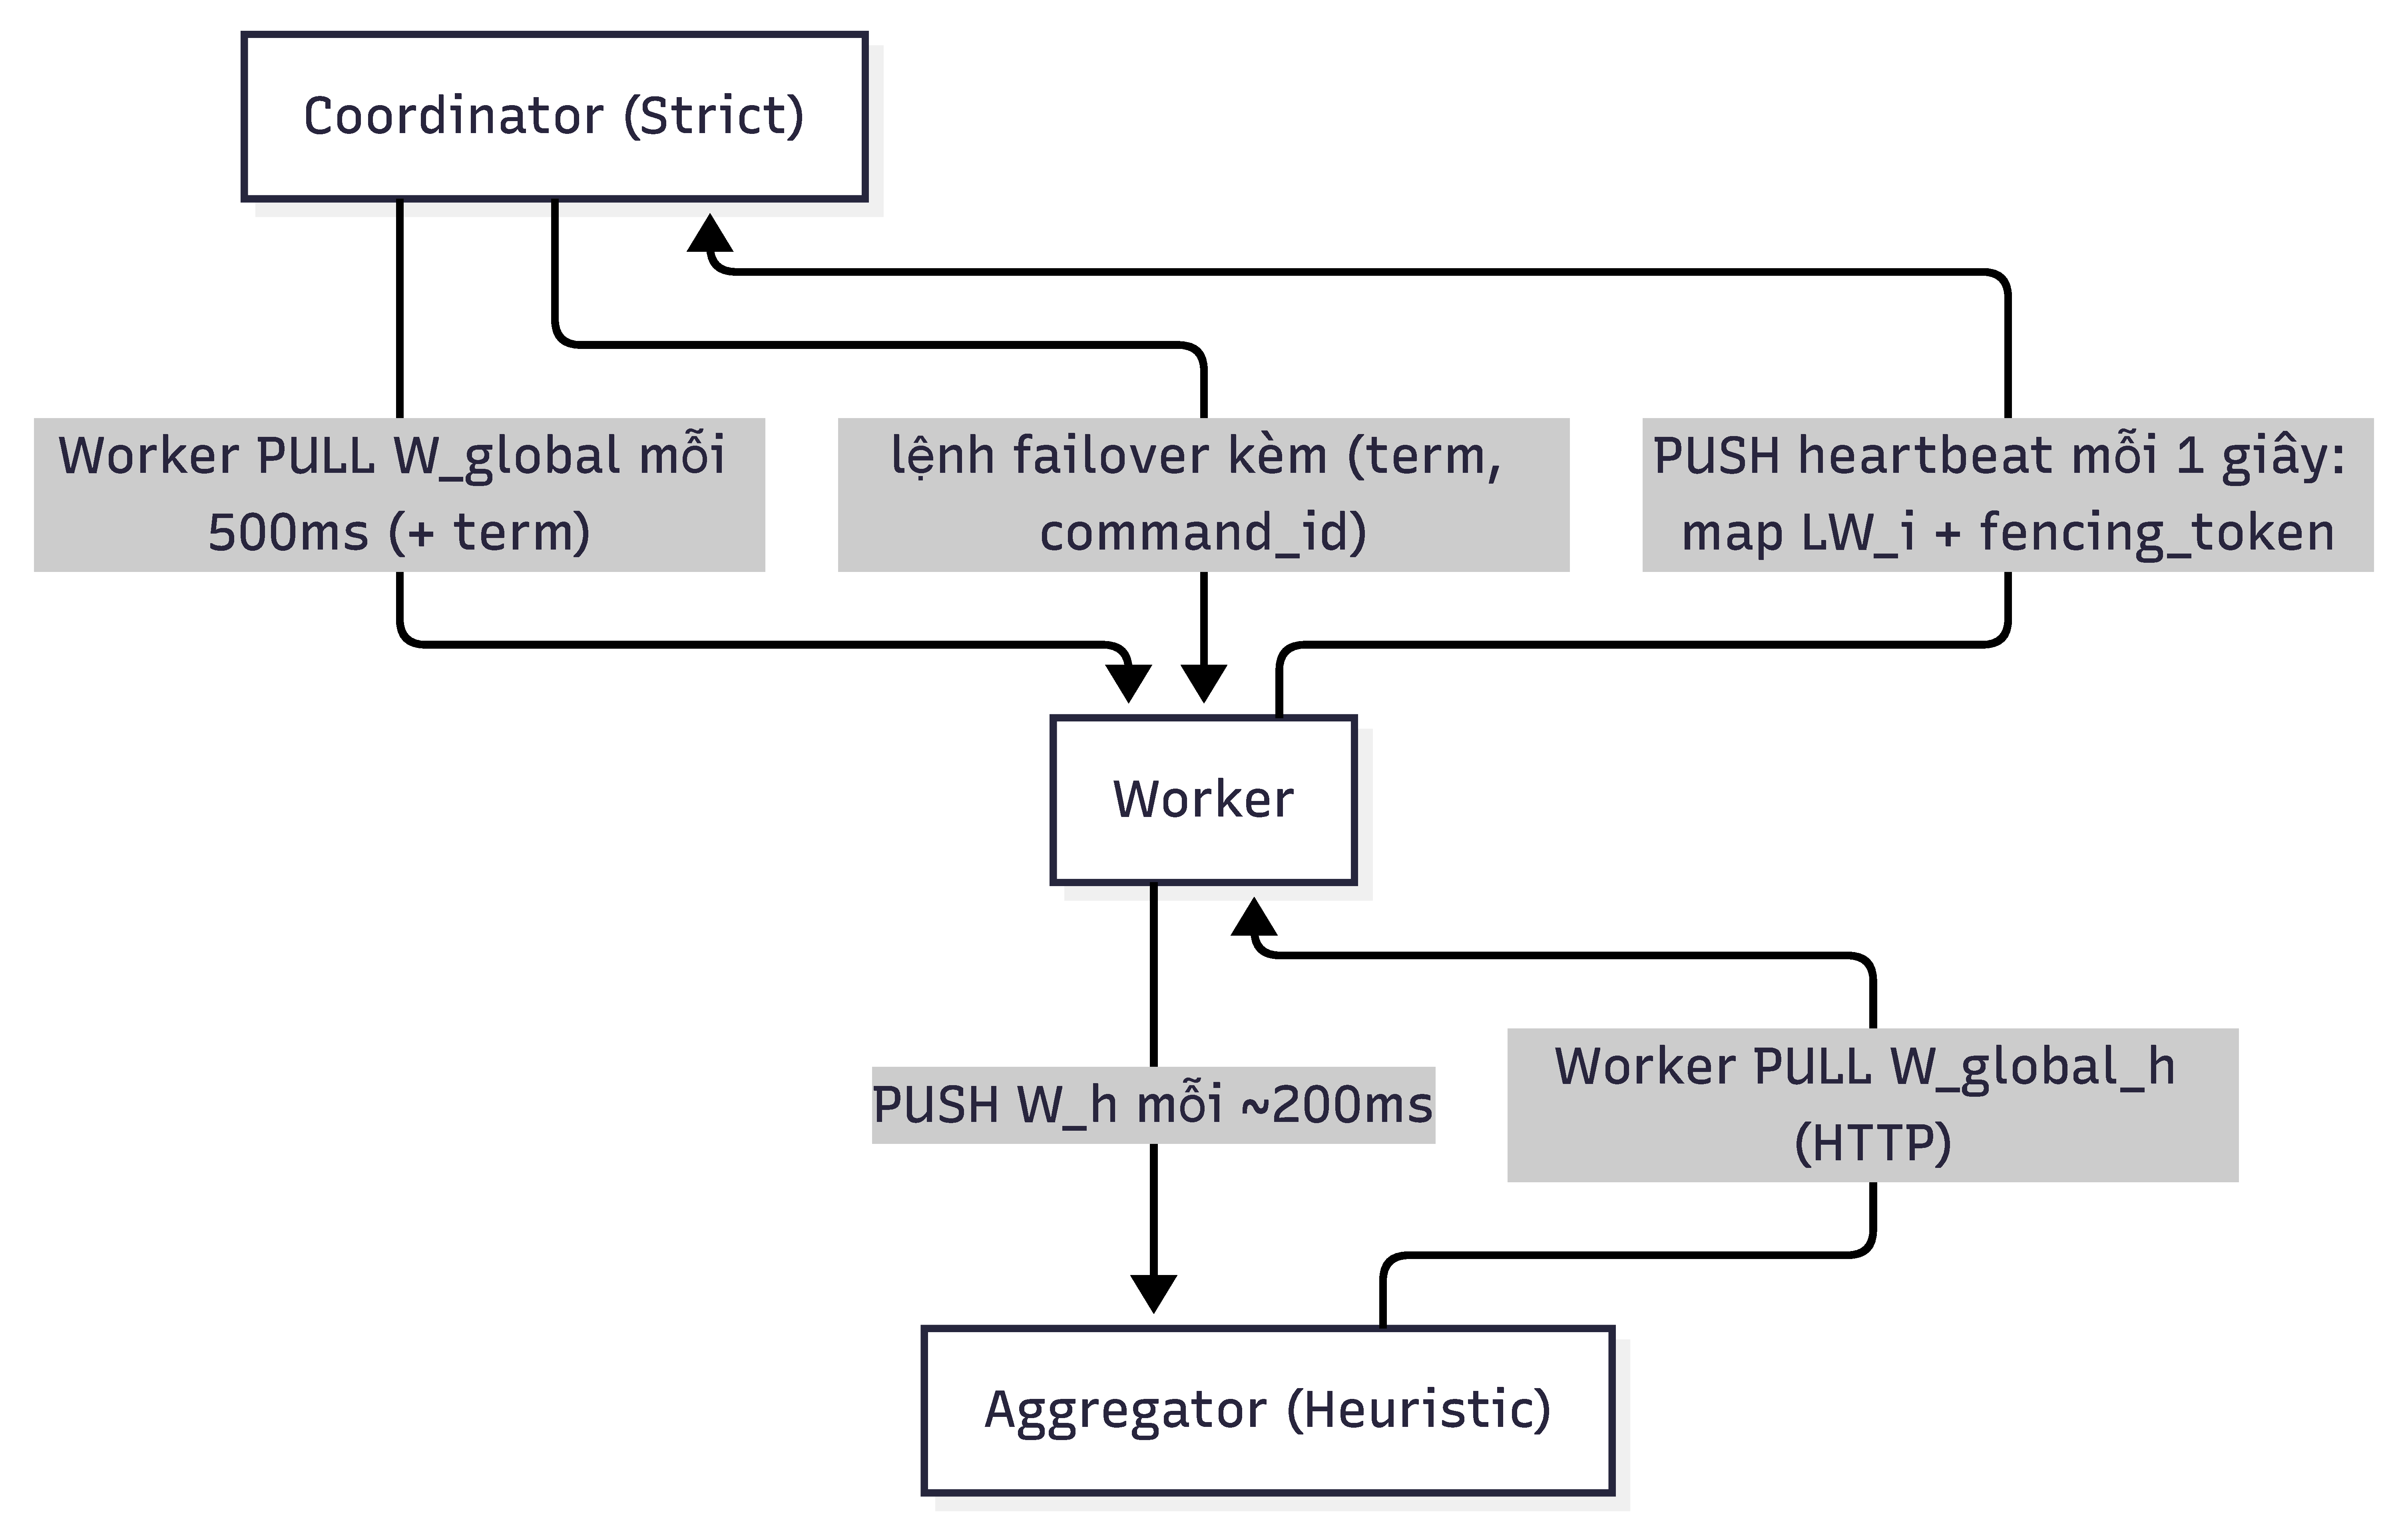
\includegraphics[width=1.15\textwidth]{comm_control_plane.pdf}}
    \caption{Sơ đồ tầng điều khiển (Worker $\leftrightarrow$ Coordinator/Aggregator)}
    \label{fig:comm_control_plane}
\end{figure}
\textbf{HTTP observability/control phụ.}

\begin{itemize}
\item \textbf{Payload:} health, state, metrics, dashboard và fallback control.
\item \textbf{Người gửi:} dashboard, operator hoặc script vận hành.
\item \textbf{Người nhận:} service endpoint.
\item \textbf{Yêu cầu chính:} dễ quan sát, dễ gọi thủ công, không nằm trên hot path.
\end{itemize}
\textbf{Storage client.}

\begin{itemize}
\item \textbf{Payload:} state, checkpoint, archive object.
\item \textbf{Người gửi:} Worker hoặc recovery process.
\item \textbf{Người nhận:} RocksDB, Tier-2 checkpoint storage, MinIO.
\item \textbf{Yêu cầu chính:} persistence ngoài RAM và phục hồi được sau lỗi.
\end{itemize}
\textbf{Luồng độc lập.}

\begin{itemize}
\item \textbf{Data plane:} event lớn đi Kafka.
\item \textbf{Control plane:} heartbeat/watermark đi gRPC.
\item \textbf{Observability:} dashboard/metrics đi HTTP.
\item \textbf{State plane:} state/checkpoint/archive đi storage client.
\end{itemize}
\textbf{Đầu ra.}

\begin{itemize}
\item \textbf{Đường dữ liệu rõ:} event đi Kafka.
\item \textbf{Đường điều khiển rõ:} watermark/heartbeat đi gRPC.
\item \textbf{Đường quan sát rõ:} health/metrics đi HTTP.
\item \textbf{Đường state rõ:} RocksDB/Tier-2/MinIO giữ state.
\end{itemize}
\textbf{Bản đồ giao tiếp theo kênh.}

\begin{table}[H]
\centering
\begin{tabular}{p{2.5cm}p{2.2cm}p{2.2cm}p{2.2cm}p{5.5cm}}
\toprule
\textbf{Kênh} & \textbf{Ai gửi/nhận} & \textbf{Payload} & \textbf{Nhịp hoạt động} & \textbf{Khi lỗi thì sao} \\
\midrule
Kafka data plane & Ingestor -> Worker; Worker -> result/audit/DLQ & Event, punctuation, output, late event & Theo luồng dữ liệu, bền theo \tcbhighmath{offset} & Worker có thể replay từ \tcbhighmath{offset}, broker tiếp tục giữ log khi Worker pause \\
gRPC control plane & Worker -> Coordinator/Aggregator; Coordinator -> Worker & Heartbeat, watermark, Raft vote/state, lệnh reassign/failback & Chu kỳ ngắn, latency thấp & Timeout biến thành tín hiệu failover hoặc active/standby takeover \\
HTTP observability & Dashboard/operator -> service & Health, state, metrics, control fallback & Không nằm trên hot path & Lỗi HTTP không làm mất event; chỉ giảm khả năng quan sát/thao tác \\
Storage client & Worker -> RocksDB/Tier-2/MinIO & State, checkpoint, archive object & Theo event, timer hoặc window close & Retry/checkpoint/replay bảo vệ state và output \\
\bottomrule
\end{tabular}
\end{table}
\textbf{Luồng giao tiếp tổng hợp.} Với Strict, event và punctuation đi qua Kafka; Worker gửi heartbeat watermark qua gRPC; Coordinator trả \tcbhighmath{W_{global}}; Worker đóng window rồi ghi result/audit. Với Heuristic, event vẫn đi qua Kafka; Worker gửi \tcbhighmath{W_h} lên Aggregator; late event đi qua DLQ Kafka; correction cũng là một luồng dữ liệu riêng. Nhờ tách kênh, một batch event lớn không làm nghẽn heartbeat, và lỗi dashboard HTTP không làm mất dữ liệu.
\textbf{Ví dụ vận hành.}

\begin{itemize}
\item \textbf{Tình huống quá tải dữ liệu (Data Spikes) trên Data Plane:}
\item Ingestor đẩy 100,000 log/s vào Kafka topic \texttt{events}. Kafka hoạt động ổn định nhờ cơ chế lưu trữ phân vùng bền vững.
\item Bộ nhớ của Worker bị quá tải do min-heap đầy. Worker lập tức kích hoạt backpressure, phát tín hiệu pause consumer Kafka cho partition đó. Kafka broker vẫn nhận log bình thường và lưu trữ an toàn, Worker tạm dừng đọc.
\item Trong suốt thời gian Worker dừng consume log từ Kafka, Worker vẫn gửi heartbeat gRPC đều đặn mỗi 1s lên Coordinator thông qua kênh điều khiển (Control Plane). Nhờ đi đường out-of-band riêng, Coordinator biết Worker vẫn hoạt động bình thường, không kích hoạt cơ chế failover nhầm lẫn.
\item Đồng thời, người vận hành vẫn truy cập Dashboard Web qua cổng HTTP (Observability Plane) để theo dõi các metric biểu đồ thời gian thực mà không gặp bất kỳ hiện tượng lag hay mất kết nối nào.
\end{itemize}

\begin{figure}[H]
    \centering
    \makebox[\textwidth][c]{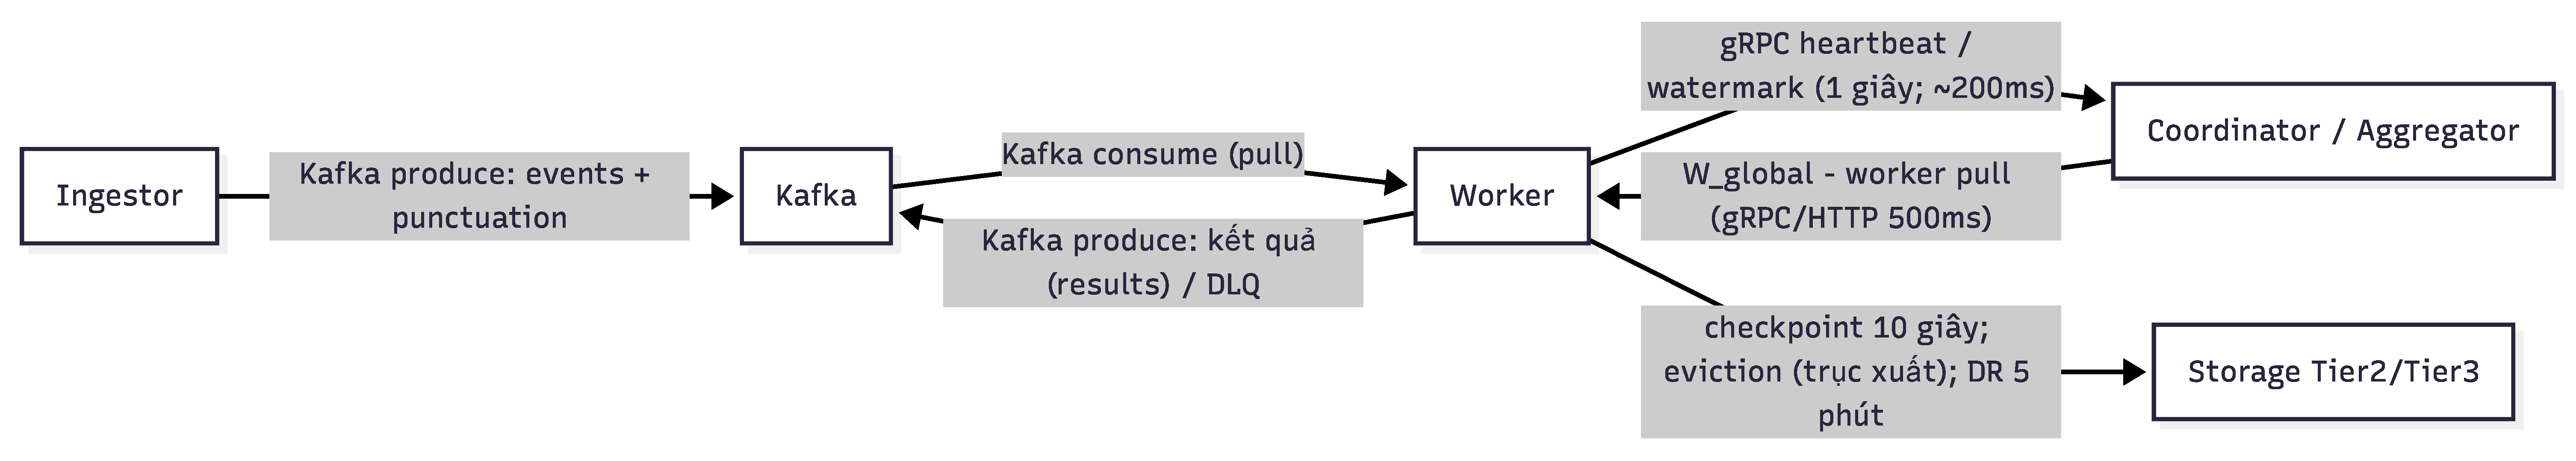
\includegraphics[width=1.15\textwidth]{layer_communication.pdf}}
    \caption{Sơ đồ}
    \label{fig:layer_communication}
\end{figure}
\textbf{Liên hệ.} Đây là mạch nối mọi mục: data plane chở event của \ref{sec:kafka-pq}, control plane chở watermark của \ref{sec:strict-watermark}/\ref{sec:heuristic-watermark}/\ref{sec:coordinator-aggregator}, state plane chở checkpoint của \ref{sec:tiered-storage}. Việc tách kênh giải thích vì sao backlog dữ liệu (\ref{sec:kafka-pq}) không làm chậm phát hiện lỗi và failover (\ref{sec:coordinator-aggregator}, \ref{sec:failback-5step}).

\subsection{7.2 Phản biện: Vì sao thiết kế như vậy}
Mục giao tiếp giữa các layer phải chỉ rõ nguyên tắc chọn kênh: không chọn theo thói quen, mà chọn theo yêu cầu của payload: bền, nhanh, quan sát được hay phục vụ state.
\textbf{Phản đề 1: Dùng HTTP cho toàn bộ hệ thống để dễ debug.}

\begin{itemize}
\item \textbf{Vì sao nghe hợp lý:} HTTP phổ biến, dễ gọi thử, dễ xem log request/response và không cần nhiều loại client.
\item \textbf{Lý do bác bỏ:} event stream cần durability, partitioning và replay bằng \tcbhighmath{offset}; HTTP request trực tiếp không cung cấp các thuộc tính này. Heartbeat/watermark lại cần schema chặt và latency thấp; dùng HTTP đồng bộ cho mọi thứ dễ làm control plane bị nghẽn cùng data plane.
\item \textbf{Kết luận phản biện:} HTTP chỉ phù hợp health/state/metrics/dashboard, không phù hợp thay Kafka data plane hoặc gRPC control plane.
\end{itemize}
\textbf{Phản đề 2: Đưa heartbeat/watermark chung vào Kafka cho thống nhất.}

\begin{itemize}
\item \textbf{Vì sao nghe hợp lý:} Kafka đã bền và có topic, đưa mọi message vào Kafka giúp một đường truyền duy nhất.
\item \textbf{Lý do bác bỏ:} heartbeat và watermark là tín hiệu điều khiển tần suất cao, cần phản hồi nhanh để phát hiện failover. Nếu control message nằm chung cơ chế backlog với event, lúc Kafka backlog lớn thì control plane cũng chậm theo, làm phát hiện lỗi và cập nhật watermark bị trễ.
\item \textbf{Kết luận phản biện:} data plane đi Kafka; control plane đi gRPC out-of-band để không bị dữ liệu lớn làm nghẽn.
\end{itemize}
\textbf{Phản đề 3: Coordinator nên push \tcbhighmath{W_{global}} đến Worker thay vì Worker pull.}

\begin{itemize}
\item \textbf{Vì sao nghe hợp lý:} push có vẻ realtime hơn; khi watermark đổi, Coordinator gửi ngay cho Worker.
\item \textbf{Lý do bác bỏ:} push buộc Coordinator quản lý trạng thái kết nối tới mọi Worker và xử lý lại khi Leader đổi. Nếu Worker mất kết nối tạm thời, logic retry/ordering phức tạp hơn. Pull giúp Worker tự nhịp, Leader đổi thì Worker chỉ cần gọi endpoint hiện tại để lấy state mới.
\item \textbf{Kết luận phản biện:} Worker pull \tcbhighmath{W_{global}} đơn giản hơn cho HA và đủ tốt với chu kỳ ngắn như 500ms.
\end{itemize}
\textbf{Phản đề 4: Ingestor gửi heartbeat trực tiếp bằng gRPC vào Coordinator.}

\begin{itemize}
\item \textbf{Vì sao nghe hợp lý:} Coordinator nhận tín hiệu trực tiếp, không cần thêm topic/luồng trung gian.
\item \textbf{Lý do bác bỏ:} nhiều Ingestor fan-in vào một endpoint Coordinator có thể tạo điểm nghẽn. Khi Coordinator đổi Leader, toàn bộ Ingestor phải cập nhật kết nối. Đưa heartbeat Ingestor qua luồng Kafka riêng giúp hấp thụ burst và giữ lại lịch sử tín hiệu.
\item \textbf{Kết luận phản biện:} Ingestor-heartbeat qua Kafka giúp giảm fan-in trực tiếp và làm control path ổn định hơn.
\end{itemize}

\section{8. Thiết kế Failback 5 bước}
\label{sec:failback-5step}

\subsection{8.1 Trình bày chi tiết thiết kế}
\textbf{Ý chính.} Failback là quy trình đưa partition từ worker đang gánh hộ về worker cũ đã phục hồi. Worker cũ không được tự mở lại partition. Coordinator điều phối bàn giao qua 5 bước tuần tự: \texttt{PAUSE -> FLUSH\_ACK -> KAFKA\_REASSIGN -> SEEK\_RESUME -> COMPLETE}. Mỗi partition đi theo máy trạng thái \texttt{ASSIGNED -> REASSIGNING -> PAUSED -> ASSIGNED}.
\textbf{Bản đồ thiết kế.}
\textbf{Thành phần và trách nhiệm.}

\begin{itemize}
\item \textbf{Coordinator Leader:} điều phối toàn bộ failback và ghi tiến độ vào control plane.
\item \textbf{Worker đang gánh hộ:} đang sở hữu tạm partition sau failover, cần pause và flush.
\item \textbf{Worker hồi phục:} worker cũ muốn nhận lại partition, chỉ được resume sau khi được cấp owner.
\item \textbf{Kafka consumer:} cần pause/seek/resume đúng \tcbhighmath{offset}.
\item \textbf{Checkpoint storage:} giữ state và \tcbhighmath{offset} an toàn trước khi chuyển owner.
\item \textbf{Failback state machine:} lưu step hiện tại để tiếp tục nếu leader đổi giữa chừng.
\end{itemize}
\textbf{Dữ liệu điều phối vào.}

\begin{itemize}
\item \textbf{Partition id:} partition cần trả về.
\item \textbf{From-worker:} worker đang gánh hộ.
\item \textbf{To-worker:} worker hồi phục sẽ nhận lại partition.
\item \textbf{Offset cuối:} \tcbhighmath{offset} an toàn sau khi flush.
\item \textbf{Ack từng bước:} xác nhận từ worker để Coordinator chuyển step.
\end{itemize}
\textbf{Dữ liệu điều phối ra.}

\begin{itemize}
\item \textbf{Lệnh \texttt{PAUSE}:} yêu cầu worker gánh hộ dừng consume.
\item \textbf{Lệnh \texttt{KAFKA\_REASSIGN}:} đổi owner partition.
\item \textbf{Lệnh \texttt{SEEK\_RESUME}:} yêu cầu worker hồi phục đọc checkpoint và seek Kafka.
\item \textbf{Term/command id:} metadata chống lệnh cũ và lệnh trùng.
\end{itemize}
\textbf{Trạng thái cần giữ.}

\begin{itemize}
\item \textbf{Failback step:} \texttt{PAUSE}, \texttt{FLUSH\_ACK}, \texttt{KAFKA\_REASSIGN}, \texttt{SEEK\_RESUME}, \texttt{COMPLETE}.
\item \textbf{Partition state:} \texttt{ASSIGNED}, \texttt{REASSIGNING}, \texttt{PAUSED}, rồi quay lại \texttt{ASSIGNED}.
\item \textbf{Pending reassignment:} partition đang chuyển từ worker nào sang worker nào.
\item \textbf{Persisted failback state:} bản ghi bền để leader mới tiếp tục đúng step.
\end{itemize}
\textbf{Giao tiếp.}

\begin{itemize}
\item \textbf{Coordinator -> worker gánh hộ:} gửi \texttt{PAUSE} và yêu cầu flush.
\item \textbf{Worker gánh hộ -> Coordinator:} trả \texttt{FLUSH\_ACK} kèm checkpoint id và \tcbhighmath{offset} cuối.
\item \textbf{Coordinator -> worker hồi phục:} gửi \texttt{SEEK\_RESUME}.
\item \textbf{Worker hồi phục -> Coordinator:} ack đã đọc checkpoint và resume đúng \tcbhighmath{offset}.
\item \textbf{Coordinator -> control plane/Raft log:} ghi step mới sau mỗi ack hợp lệ.
\end{itemize}
\textbf{Đầu ra.}

\begin{itemize}
\item \textbf{Owner cuối:} partition trở về worker hồi phục.
\item \textbf{Offset continuity:} worker hồi phục đọc tiếp từ \tcbhighmath{offset + 1}.
\item \textbf{Không duplicate owner:} không có thời điểm hai worker cùng consume partition.
\item \textbf{Failback state sạch:} state tạm được xóa khi \texttt{COMPLETE}.
\end{itemize}
\textbf{Thiết kế failover trước khi failback.}
\textbf{Mục tiêu.}

\begin{itemize}
\item \textbf{Phục hồi nhanh khi Worker chết:} partition của Worker lỗi phải có owner mới.
\item \textbf{Không có hai owner cùng lúc:} partition orphaned chỉ được gán cho một Worker sống.
\item \textbf{Không mất \tcbhighmath{offset}/state:} Worker nhận thay phải đọc checkpoint và seek Kafka đúng vị trí.
\end{itemize}
\textbf{Tín hiệu phát hiện lỗi.}

\begin{itemize}
\item \textbf{Heartbeat timeout:} Worker không gửi heartbeat quá ngưỡng.
\item \textbf{Partition stale:} partition không có watermark/\tcbhighmath{offset} mới trong thời gian cho phép.
\item \textbf{Consumer lag bất thường:} lag tăng nhưng Worker không phản hồi.
\item \textbf{Control command timeout:} lệnh pause/flush/reassign không được ack.
\end{itemize}
\textbf{Dữ liệu failover cần có.}

\begin{itemize}
\item \textbf{Failed worker id:} Worker bị đánh dấu lỗi.
\item \textbf{Orphaned partitions:} danh sách partition đang thuộc Worker lỗi.
\item \textbf{Last safe checkpoint:} checkpoint mới nhất đọc được từ Tier-2.
\item \textbf{Last safe \tcbhighmath{offset}:} \tcbhighmath{offset} đi kèm checkpoint.
\item \textbf{Target worker:} Worker sống được chọn để gánh hộ.
\item \textbf{Owner epoch/\tcbhighmath{term}:} metadata fencing cho owner mới.
\end{itemize}
\textbf{Luồng failover.}

\begin{enumerate}
\item Coordinator phát hiện Worker lỗi qua heartbeat timeout.
\item Coordinator đánh dấu Worker là \texttt{FAILED}.
\item Coordinator lấy danh sách partition của Worker lỗi và đánh dấu chúng là orphaned.
\item Coordinator chọn Worker sống để nhận từng partition orphaned.
\item Worker mới đọc checkpoint Tier-2 của partition được giao.
\item Worker mới mở engine/state và seek Kafka từ \texttt{last\_safe\_\tcbhighmath{offset + 1}}.
\item Coordinator cập nhật owner/epoch mới và ghi trạng thái partition là \texttt{ASSIGNED}.
\item Worker mới bắt đầu consume, xử lý tiếp phần log sau checkpoint.
\end{enumerate}
\textbf{Trạng thái sau failover.}

\begin{itemize}
\item \textbf{Owner tạm thời:} Worker gánh hộ trở thành owner hợp lệ.
\item \textbf{Checkpoint được dùng:} hệ thống biết checkpoint nào đã dùng để phục hồi.
\item \textbf{Offset tiếp tục:} Kafka consumer bắt đầu từ \tcbhighmath{offset} an toàn.
\item \textbf{Failback candidate:} Worker cũ nếu hồi phục sẽ không tự lấy lại partition, mà phải đi qua failback 5 bước.
\end{itemize}
\textbf{Quan hệ giữa failover và failback.}

\begin{itemize}
\item \textbf{Failover:} xảy ra khi Worker chết, mục tiêu là giữ hệ thống tiếp tục chạy.
\item \textbf{Failback:} xảy ra sau khi Worker cũ hồi phục, mục tiêu là trả partition về owner mong muốn.
\item \textbf{Điểm nối:} failback chỉ bắt đầu sau khi failover đã tạo owner tạm thời hợp lệ và checkpoint/\tcbhighmath{offset} của owner tạm thời đã rõ.
\end{itemize}
\textbf{Bản đồ 5 bước failback.}

\begin{table}[H]
\centering
\begin{tabular}{p{1.5cm}p{2.8cm}p{5.7cm}p{5.0cm}}
\toprule
\textbf{Bước} & \textbf{Ai thực hiện} & \textbf{Nội dung} & \textbf{Điều kiện để sang bước tiếp theo} \\
\midrule
\texttt{PAUSE} & Coordinator gửi lệnh cho worker đang gánh hộ & Dừng consume partition đó, không nhận thêm event mới vào engine & Worker ack rằng partition đã pause và không còn poll thêm \\
\texttt{FLUSH\_ACK} & Worker đang gánh hộ & Flush RocksDB/state, ghi checkpoint Tier-2, chốt \tcbhighmath{offset} cuối an toàn & Ack trả về checkpoint id và \tcbhighmath{offset} cuối \\
\texttt{KAFKA\_REASSIGN} & Coordinator & Đổi owner partition từ worker gánh hộ sang worker hồi phục, tăng epoch/fencing \tcbhighmath{term} & Thay đổi owner được ghi bền trong control plane \\
\texttt{SEEK\_RESUME} & Worker hồi phục & Đọc checkpoint, mở lại engine/state, seek Kafka tới \tcbhighmath{offset + 1} & Worker ack đã sẵn sàng consume từ đúng \tcbhighmath{offset} \\
\texttt{COMPLETE} & Coordinator & Đánh dấu partition trở lại \texttt{ASSIGNED}, xóa failback state tạm & Không còn pending command cho partition đó \\
\bottomrule
\end{tabular}
\end{table}
\textbf{Khi failback bị ngắt giữa chừng.}
Failback state được persist theo partition, gồm step hiện tại, source worker, target worker, \tcbhighmath{offset}/checkpoint và \texttt{command\_id}. Nếu Leader đổi ở bước \texttt{FLUSH\_ACK}, Leader mới đọc state và tiếp tục từ \texttt{FLUSH\_ACK}, không quay lại từ đầu. Nếu cùng một lệnh được gửi lại, Worker nhìn \texttt{command\_id} để bỏ qua lệnh trùng. Nếu worker hồi phục lại chết trong lúc \texttt{SEEK\_RESUME}, Coordinator có thể giữ partition ở worker gánh hộ hoặc mở failover mới tùy trạng thái committed cuối cùng.
\textbf{Ví dụ vận hành.}

\begin{itemize}
\item \textbf{Quy trình đưa partition \texttt{P4} từ Worker gánh hộ \texttt{W2} trở về Worker cũ \texttt{W1} đã phục hồi:}
\item \textbf{Bước 1 (PAUSE):} Coordinator gửi lệnh pause partition \texttt{P4} kèm \tcbhighmath{term} = 5 và \texttt{command\_id} = 101 cho \texttt{W2}. \texttt{W2} dừng consume Kafka cho \texttt{P4} và ack lại Coordinator.
\item \textbf{Bước 2 (FLUSH\_ACK):} \texttt{W2} thực hiện flush toàn bộ open window và \tcbhighmath{offset} của \texttt{P4} xuống Tier-2 checkpoint, chốt \tcbhighmath{offset} an toàn cuối cùng là 950. \texttt{W2} gửi \texttt{FLUSH\_ACK} kèm \tcbhighmath{offset} 950 về Coordinator.
\item \textbf{Bước 3 (KAFKA\_REASSIGN):} Coordinator cập nhật bảng sở hữu partition trong control plane, gán \texttt{P4} cho \texttt{W1} và tăng \tcbhighmath{term} lên 6. Trạng thái \texttt{P4} chuyển sang \texttt{PAUSED}.
\item \textbf{Bước 4 (SEEK\_RESUME):} Coordinator gửi lệnh resume \texttt{P4} kèm \tcbhighmath{term} 6 cho \texttt{W1}. \texttt{W1} đọc checkpoint của \texttt{P4} từ Tier-2 để khôi phục state, seek consumer Kafka partition \texttt{P4} đến \tcbhighmath{offset} 951, sau đó bắt đầu đọc dữ liệu và ack lại Coordinator.
\item \textbf{Bước 5 (COMPLETE):} Coordinator nhận ack từ \texttt{W1}, chuyển trạng thái \texttt{P4} thành \texttt{ASSIGNED} và hoàn tất quy trình failback. Suốt quá trình này, \texttt{W1} và \texttt{W2} không bao giờ cùng đọc partition \texttt{P4} tại bất kỳ thời điểm nào.
\end{itemize}

\begin{figure}[H]
    \centering
    \makebox[\textwidth][c]{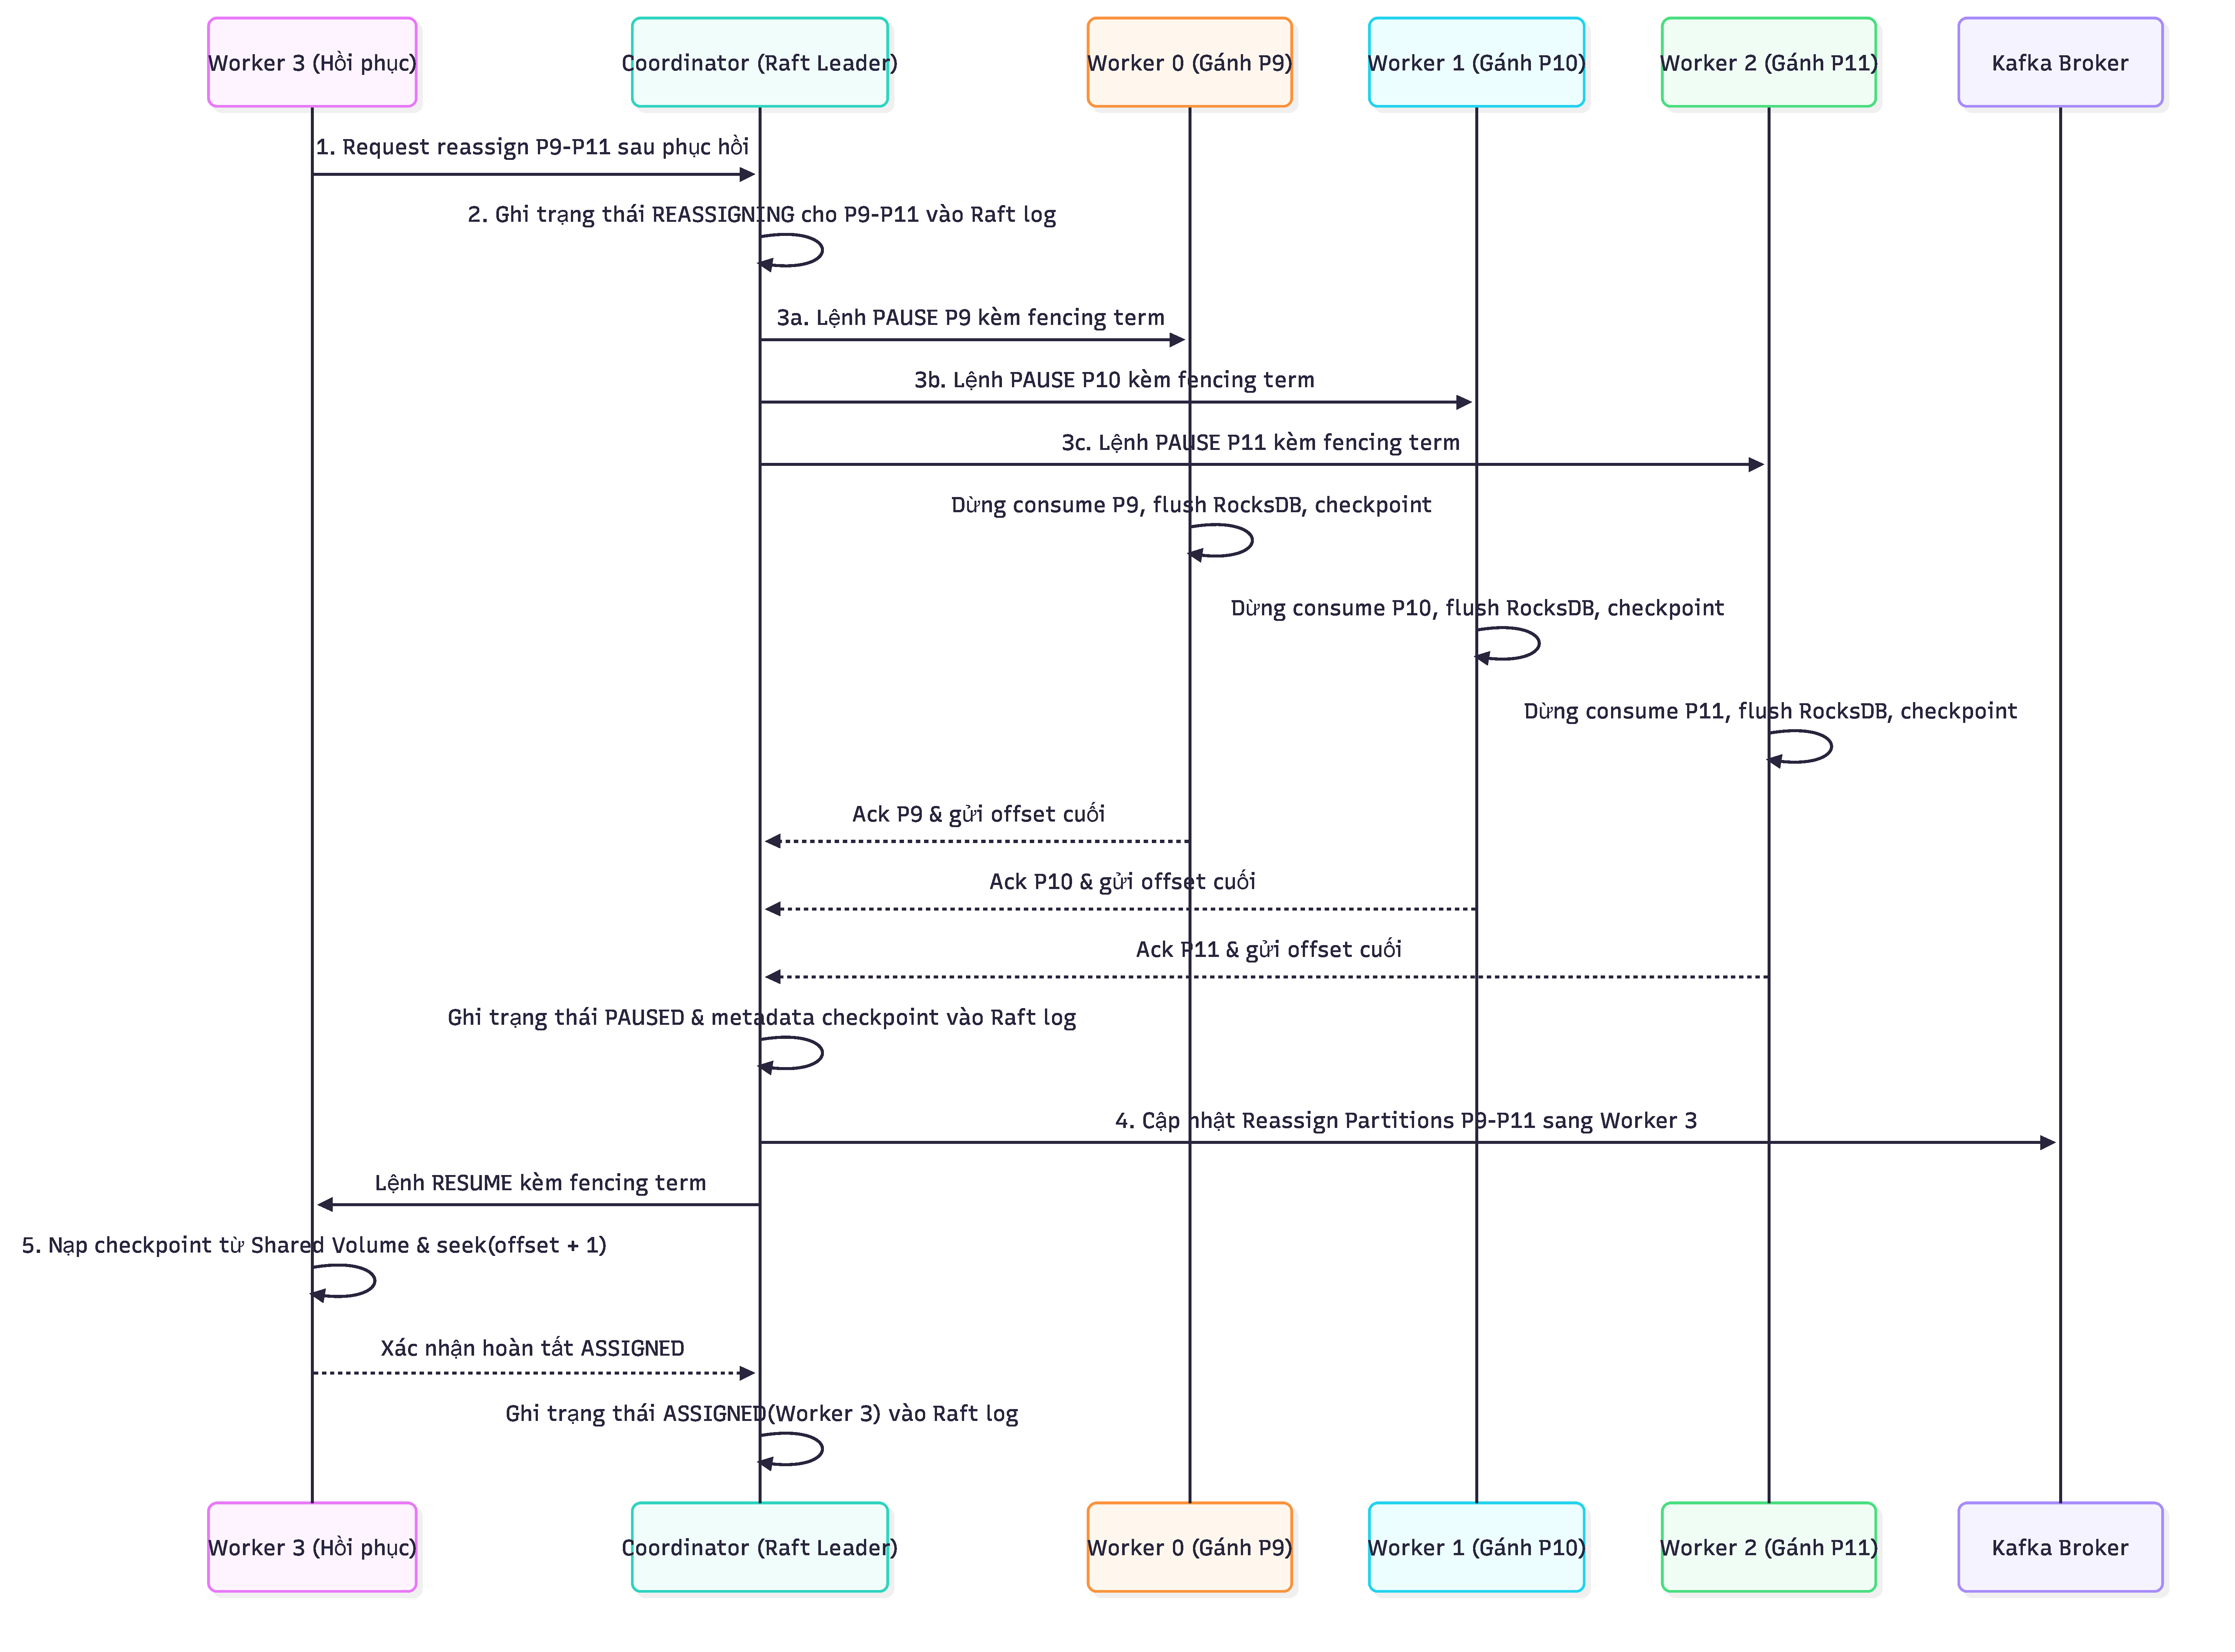
\includegraphics[width=1.15\textwidth]{failback_5step_seq.pdf}}
    \caption{Sơ đồ trình tự 5 bước}
    \label{fig:failback_5step_seq}
\end{figure}

\begin{figure}[H]
    \centering
    \makebox[\textwidth][c]{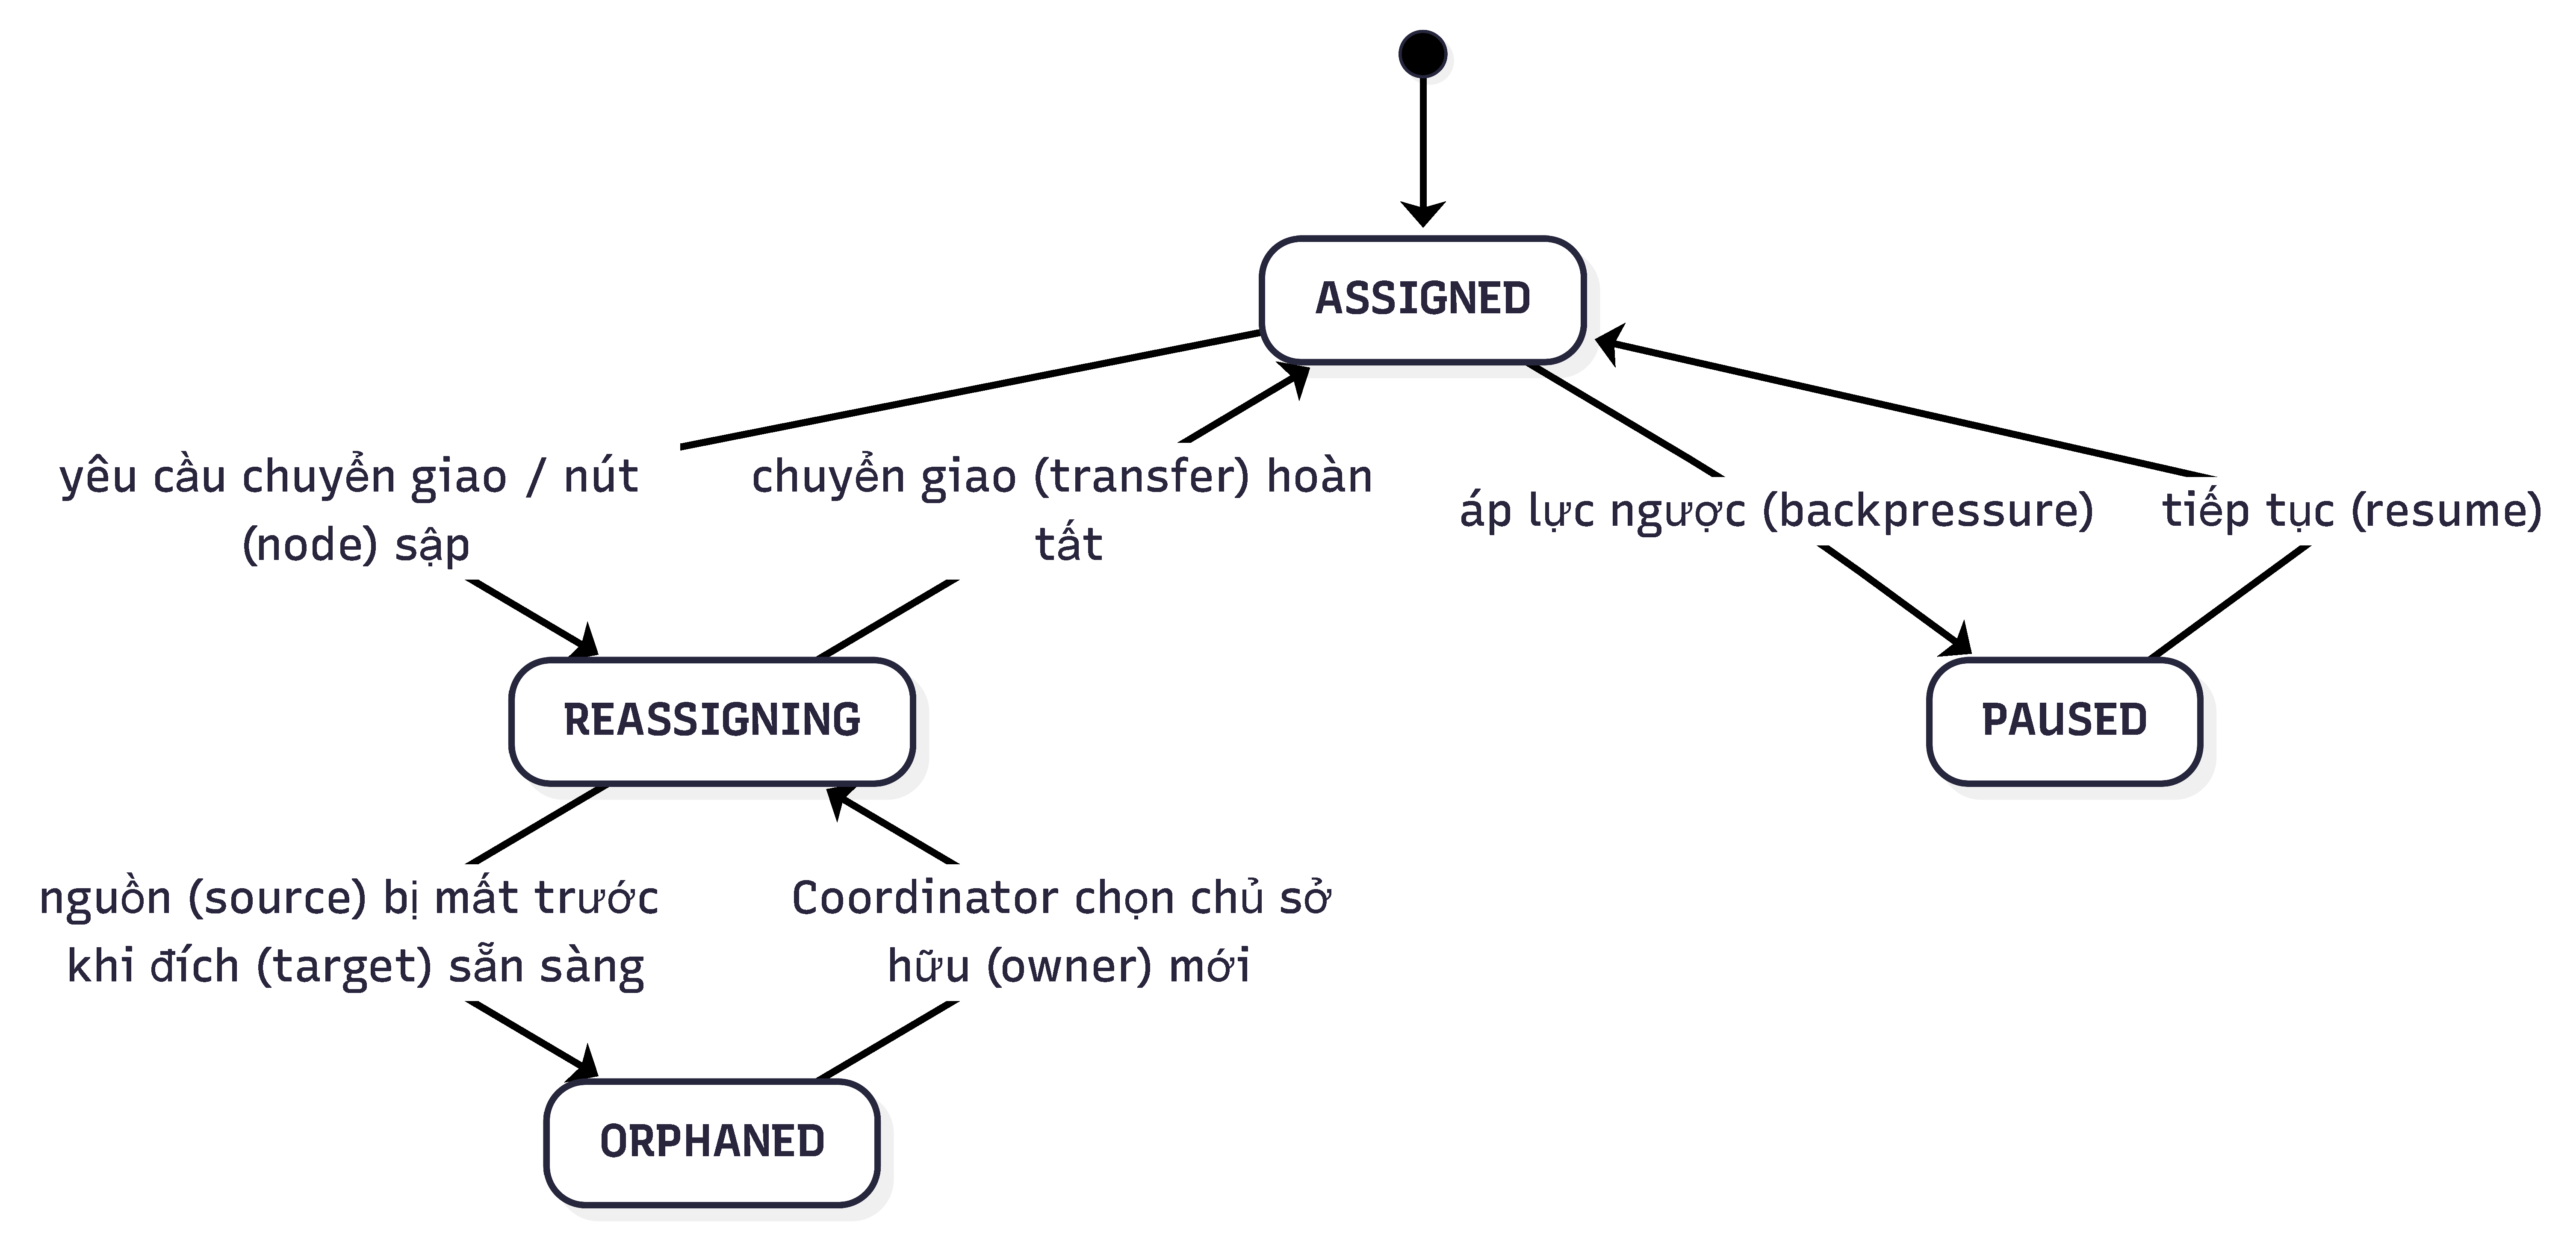
\includegraphics[width=1.15\textwidth]{partition_state_machine.pdf}}
    \caption{Máy trạng thái sở hữu partition}
    \label{fig:partition_state_machine}
\end{figure}
\textbf{Liên hệ.} Failback đứng trên ba thứ đã dựng trước đó: ownership và fencing token ở Coordinator (\ref{sec:coordinator-aggregator}), checkpoint Tier-2 + \tcbhighmath{offset} ở Tiered Storage (\ref{sec:tiered-storage}), và đơn vị partition độc lập ở \ref{sec:node-partition}. Mục tiêu cuối là giữ exactly-once mà \ref{sec:strict-watermark} cam kết.

\subsection{8.2 Phản biện: Vì sao thiết kế như vậy}
Mục Failback tập trung giải thích vì sao partition không được tự quay lại worker cũ và vì sao owner mới phải đọc tiếp từ \tcbhighmath{offset}/state an toàn.
\textbf{Phản đề 1: Worker hồi phục tự mở lại partition cũ.}

\begin{itemize}
\item \textbf{Vì sao nghe hợp lý:} partition vốn thuộc Worker đó trước khi lỗi, nên khi Worker sống lại thì cho nó nhận lại ngay sẽ nhanh hơn.
\item \textbf{Lý do bác bỏ:} trong lúc Worker cũ chết, partition có thể đã được Worker khác gánh hộ. Nếu Worker cũ tự consume lại, hệ thống có thể có hai owner cùng đọc Kafka và cùng ghi output cho một partition. Hậu quả là duplicate output, lệch \tcbhighmath{offset} và mất exactly-once.
\item \textbf{Kết luận phản biện:} worker hồi phục không được tự nhận partition; mọi chuyển giao phải qua Coordinator và fencing \tcbhighmath{term}.
\end{itemize}
\textbf{Phản đề 2: Chỉ đổi owner trong Kafka rồi cho worker mới chạy, bỏ PAUSE/FLUSH.}

\begin{itemize}
\item \textbf{Vì sao nghe hợp lý:} giảm số bước failback, partition trở về owner cũ nhanh hơn.
\item \textbf{Lý do bác bỏ:} worker đang gánh hộ có thể còn event trong buffer, state chưa flush hoặc \tcbhighmath{offset} cuối chưa ghi checkpoint. Nếu đổi owner ngay, worker mới có thể đọc từ \tcbhighmath{offset} sai: hoặc đọc lặp quá nhiều, hoặc bỏ sót phần worker cũ đã poll nhưng chưa checkpoint.
\item \textbf{Kết luận phản biện:} phải có \texttt{PAUSE} để dừng nhận thêm event và \texttt{FLUSH\_ACK} để ghi state/\tcbhighmath{offset} an toàn trước khi \texttt{KAFKA\_REASSIGN}.
\end{itemize}
\textbf{Phản đề 3: Không cần ghi từng bước vào Raft log, làm tuần tự trong RAM là đủ.}

\begin{itemize}
\item \textbf{Vì sao nghe hợp lý:} failback là quy trình ngắn; giữ state trong RAM có vẻ đơn giản hơn.
\item \textbf{Lý do bác bỏ:} Leader có thể đổi giữa chừng. Nếu state failback chỉ nằm trong RAM của Leader cũ, Leader mới không biết partition đang ở bước nào và có thể làm lại từ đầu hoặc bỏ qua bước chưa hoàn tất. Điều này tạo duplicate command hoặc chuyển owner khi \tcbhighmath{offset} chưa an toàn.
\item \textbf{Kết luận phản biện:} từng bước failback phải được persist/replicate; \tcbhighmath{term} và \texttt{command\_id} giúp từ chối lệnh cũ và bỏ qua lệnh trùng.
\end{itemize}

\end{document}
